\documentclass[twoside,11pt,a5paper]{memoir}

\usepackage[top=1.1in,bottom=0.9in]{geometry}
\usepackage{graphicx}
\usepackage{caption}
\usepackage{pdfpages}

% Preamble
\usepackage[osf]{libertine}
\usepackage{microtype}

\nouppercaseheads


% Information
\title{My Life in and around\\Thorn Moor and Beyond}
\author{Mike Saffin}
\date{}


% DOCUMENT
\begin{document}

% Front cover
% 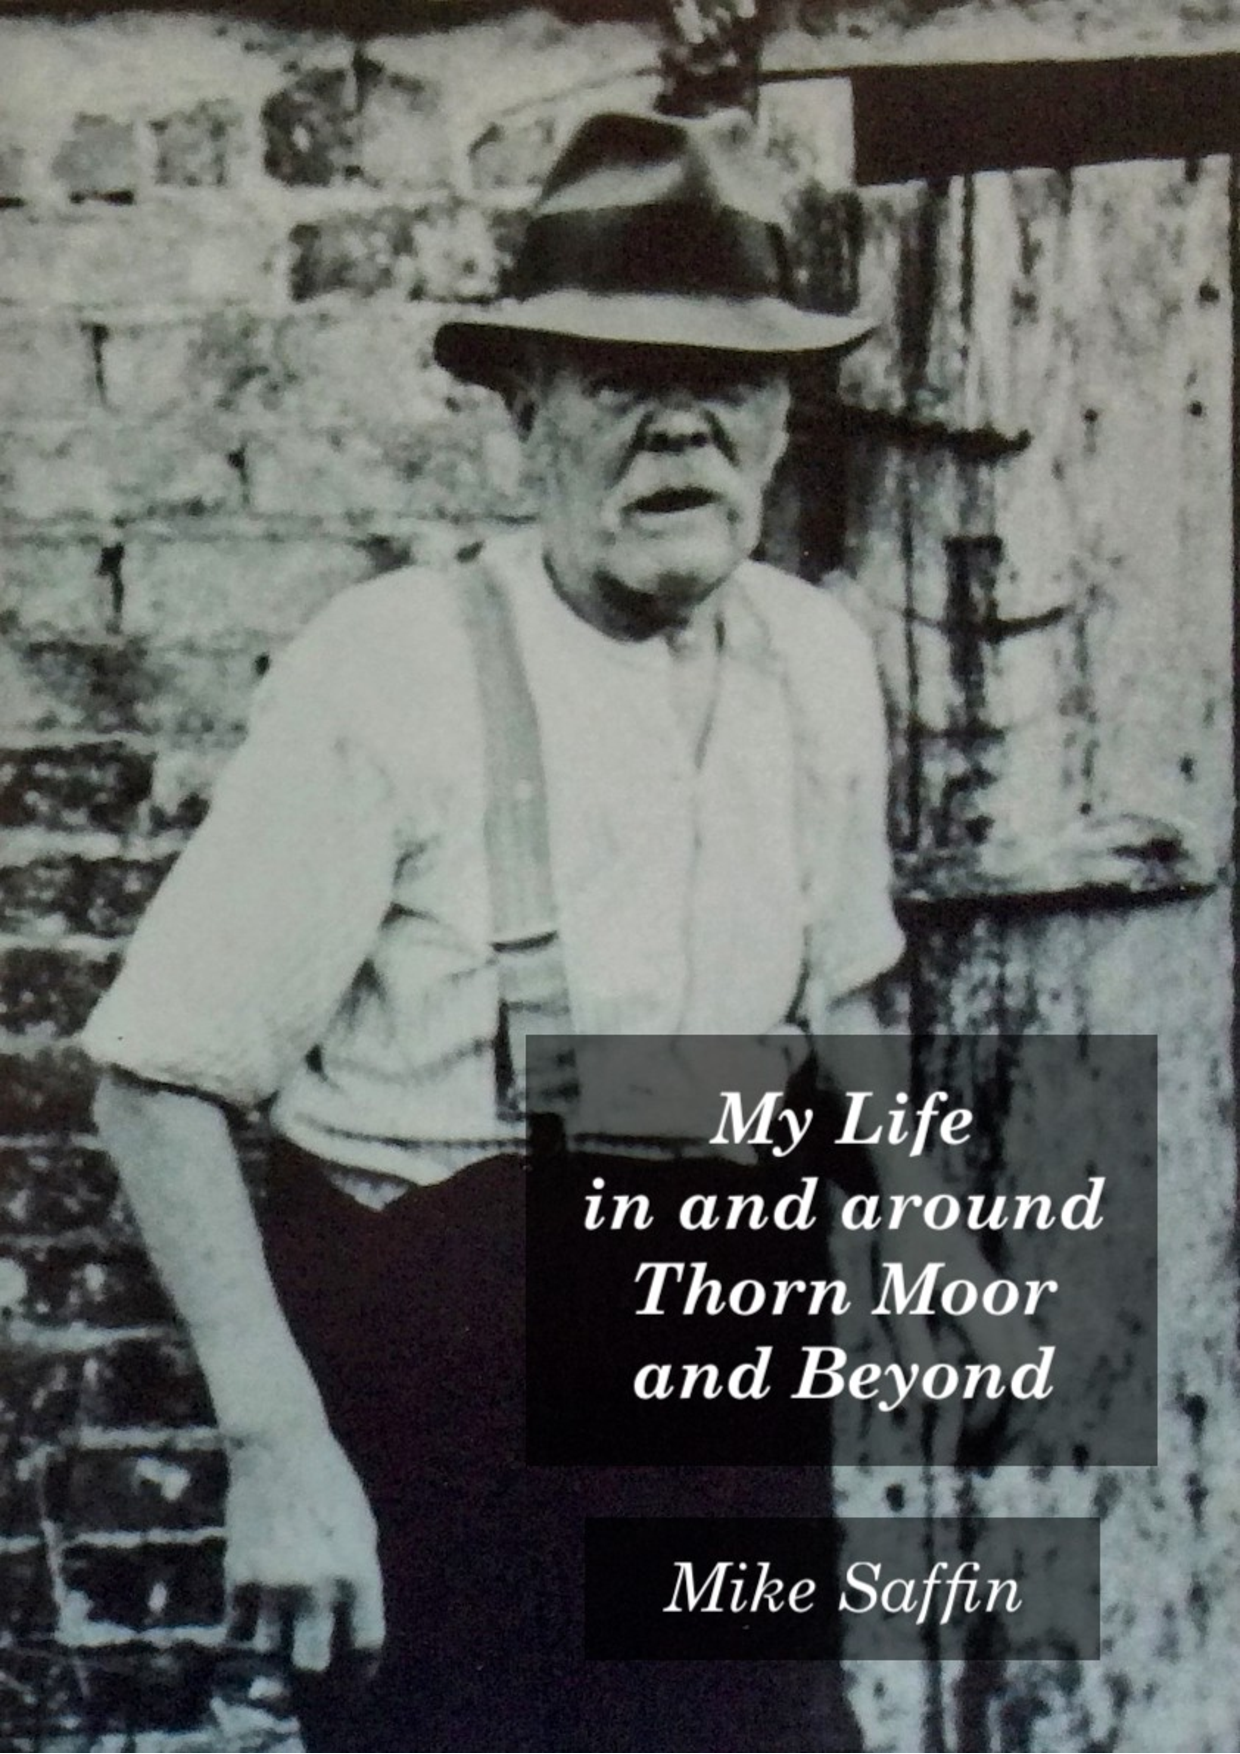
\includepdf{pictures/front-cover.pdf}

\maketitle

\chapter*{Old Devon verse}
%!TEX root = ../thorn-moor.tex


\emph{Weather and action required by farmers in the month of March.} When the
blackthorn is covered with white flowers it is called a blackthorn winter
(period of very cold east winds requiring overcoats). East wind is called a
lazy wind, too lazy to go around but blows straight through. When the
blackthorn blossom is white, till the barley day or night. March winds and
April showers bring forth May flowers.

\bigskip
\noindent Advice to youth in respect of clothing: never cast a clout until May
is out.

\bigskip
\noindent
\emph{Regarding Dartmoor weather.} When I was a young man living at home before
marriage --- location Thorn Moor Farm, in the Big Pennypark field --- looking
across the Devon countryside at 15+ miles directly into Causdon Beacon, if the
moor looked very clear and close whilst sitting at the bottom of Big
Pennypark, rain would develop in the next few hours or days and the heavy laden
rain filled-humidity would cause magnification of the moor. If the moor looked
far away and purple we would receive fine dry weather in a period of time. Home
wind blowing east: dry day; wind from the west: warmer and wet.

\bigskip
\noindent When Kirton (Crediton) was a busy market town, Exeter was nothing but
a fuzzy down.

\bigskip
\noindent Instructions from a farmer to his workmen: ``Boy! Rin, boy ride, boy
rin and tell the doctor Mrs been and poked the cow's horn in her eye!''

\bigskip
\noindent Two pigs in a house by themselves do better than one together.

\bigskip
\noindent Farmer looking over his crop of potatoes in the rain: ``this shower of
rain will spoil the little potatoes''.

\bigskip
\noindent Trouble with clocks going forward for summertime: it gets late early!


\chapter*{Foreword}

I apologise to anyone who, having read this book, has walked away thinking,
``this man is arrogant and talks about himself''. It is not intended to read
that way, as in the past 6 years I have been asked to put my life on paper
before it is lost. So I put pen to paper in the full knowledge that I have no
idea how to write a book or to put any events into the correct grammar
context! I just set forth! What is correct grammar? Define grammar --- grammar
teaches us the proper arrangement of words according to the ideals and dialects
of any particular kingdom of people. It teaches us to speak and write with
precision. Agreeable to question authority, I am a Devonian, born and bred in
Devon, so the West Country culture sits squarely on my shoulders.

I thank my wife, Vera (who is Godmother to her cousins’ daughter Emma, who was
born on the same day as her), for standing and supporting me throughout my many
years of projects. Without that support there would be nothing to write about;
also to my lifelong friend Patience who took away my scribbles to be formed
into this booklet; and most importantly to my Godson, Tim Hosgood, for his
energy and dedication in editing and bringing my story to life.

\bigskip

\emph{Mike Saffin, October 2022}

\chapter{}
%!TEX root = ../thorn-moor.tex

Thorn Moor/Tilery House nestled very comfortably in the moorland countryside
with all its beauty in the summertime, softness in spring and raw brutal
harshness of the long dark winter. However it was well blessed with farmsteads
and families that were great friends, with a community spirit that collectively
pulled us through the season, and the prospective tools required for survival.
In no particular order lies a house named Little Thorn with a Mrs Vodden and
her daughter Beattie, who both visited my mother spending time sharing area
gossip, all very light but good company. About one and a half miles away to the
south east lay Half Acre Farm, occupied in the early days by a Mrs Anstee, a
grandmother to a great friend of mine today who I shall cover later in my
story. This farm, Half Acre was then occupied by a Mr and Mrs Down who joined
in the area community spirit by Mrs Down visiting afternoons to gossip with
mother about local issues and the progress, good or bad, of the war. Mr Down
would visit evenings at about 8 o'clock in rain, snow or wind. Dad would laugh
at the order of his entry --- knocking on the back door, door would open and Mr
Down would walk straight in though the living room behind the old Devon settle
shouting ``anybody in''. Dad wondered about a response with ``No''. Much
conversation ensued covering crop growing, threshing, reed combing and market
prices. Refreshments were offered in the nature of sandwiches, tea, and a glass
of cider drawn by jug from the outer cellar. The evening stopped at
approximately 10.30 with a ``Is it that time already? I better make me way
back.'' Thorn Moor is located next to Thorn Farm and Thorn Cross on the
Cheriton Bishop Road. There is a disused tile yard and kiln within the house
purchased by John Preston Butt, Master Thatcher, which had been converted from
an active tile kiln into three double bedrooms, one single room which I used
until 10 years of age, a front parlour on right side of front door, a front
room used at Christmas on the left of front door (kiln area), kitchen with cold
water tap, walk-in larder with hooks in the ceiling to hang quarters of cured
meats, covered rear door area for clothes washing and killing pigs at times.
One divided shed: one part used for Grandfather to keep his pony in his
thatching days and the second part with a built-in still to distil cider into
calvados as well as for storing my motorbike and engine parts. The south-west
side was built with a long flat roof to accommodate four milking cows, thus
making natural use of warm animal body mass to heat up the building of weather
walls.

Travelling around in clockwise direction, approximately 3 miles as the crow
fliesm situated in the village of Crockernwell were various services --- Tom
Ching the saddler and cobbler would provide and repair new shoes, boots and
leather together with nails, scoots and studs to enable Dad to carry out
repairs at home. Tom Ching and Dad were good friends and both were members of
the Cheriton Bishop Council. Tom was the Clerk, and had copperplate
handwriting, and Dad said whilst a Parish Council meeting was in progress and
controversial subjects were discussed Tom would show distress by running his
fingers around his shirt collar to relieve excess body heat.

Standing between Ching's Saddlers and the pub, then the Royal Hotel, was a
wheelwright and hardware store owned by Reg Stanbury, the son of a world-famous
clay pigeon shooter. People including ourselves would visit Reg at all times of
the day to purchase a vast variety of working items: a dry battery for the
radio, rabbit wires, axes, bicycle tyres, nails and screws. The visit incurred
the same format --- knocking and entering the workshop. Reg was normally working
at his work bench and the initial conversation was always the family health
followed by the present day weather. Nothing further happened until a well-worn
shiny tobacco tin was removed from the top of his bib and brace overalls and a
very carefully rolled cigarette had been prepared and lit. Then action
commenced with the following words ``let's go and see what we've got for
you''.

The village pub, The Royal Hotel, was tended by a Mr Tom Edwards over the war
years. It later passed to the hands of David Sibbles, his wife, Irene, and his
mother. They transformed the old look to a very new and at the time modern look
to include a cafeteria in the large main hall. They subsequently obtained a
contract with the Royal Blue coaches, usually passing through to Cornwall, for
the drivers to have their required breaks and passengers to receive refreshment
including sometimes overnight stays, sometimes shorter mid-day or comfort
breaks. They were one of the very few establishments locally to install a juke
box, which attracted hoards of teenagers from miles around, mostly on Saturday
and Sunday evenings. At the top of the village was a garage owned by a Mr
Watts, who would attend my home driving an Armstrong Siddley car wearing a
shiny peaked chauffeur's cap and delivering John Preston Butt to his daughter,
Hilda, at Kenton for a holiday. After some years the garage name was changed to
Crockernwell Motors and a new proprietor came in named Jim Sharp. The nature of
the workshop changed with a great deal of fun attached to the overhaul
operation. Jim would take a chance on anything with little regard for Health
and Safety and as I used to help him of an evening for extra cash my attitude
was as a young man equally maverick. One evening I arrived at the garage and
Jim greeted me full of smiles and said ``I've got just the job for you! We
have a car to rescue from suicide corner near the Bay Tree Motel.'' On arrival
we found an Austin A35 had failed to negotiate the bend and had finished its
journey 15' up the bank wedged at an angle between two hazel bushes. I then sat
in the driver's seat whilst Jim in a Land Rover towed us off. At this stage
quite a crowd had gathered to view the action. I have no idea how the car
remained on its four wheels but it did. I was told that the gathered crowd was
a little disappointed that the Austin did not turn over. However, much back
slapping was rendered to all. Moving down to Hooperton Cross road and turning
into Thorn Road, we find Hooperton Farm. When I was a small boy I remember it
was farmed by Mr and Mrs Wreford until age forced them to retire and move to a
bungalow in Cheriton Bishop. A Mr and Mrs Wotton and their son, Francis, became
well-known walking in the area training their greyhounds. He would take me out
on a dark blustery evening and taught me the skill of catching rabbits with a
spot lamp and whippet. He was well skilled in the art of rabbit netting with a
ferret. Unfortunately Francis' happy lifestyle ended in such a tragic manner
that I am not prepared to expand any further.

The next farm is Bowden which was always very popular with small boys. When
walking by with Mum and Dad we saw a well-rotted tree stump which had twisted
into the shape of a dragon's head, and with the able assistance of outside help
had an interior red painted mouth and a red rubber tongue hanging out and two
carefully placed cycle reflectors to illuminate the eyes. This savage beast
came alive at night when passing car lights flashed by. The owners of Bowden
were Donald Seagus and his son. I lived in heaven as evenings I was lent a
BSA.22 five clip rifle. This might shock some people as I was only 14 years of
age. As we were country boys, my father taught the very strictest rules for
handling a firearm at the age of 10. He always told us never to point a gun at
anyone, no matter who, and told us to remember that more people were killed
with an empty gun, and to always walk with the gun open until required. When
handed a gun he told us to always open the breech to ensure no bullets were
within and to always keep the magazine out of the gun until needed.

%!TEX root = ../thorn-moor.tex

Walking up the hill to the crossroads we have Hask Lane, a corner of which was
purchased by a young Scotsman known as Jock who set up home by building his own
small house in the corner of the field. It commanded wonderful views of Causdon
Beacon in the distance. Jock drove a three-wheeled BSA car and was known to
stand outside his house in the evening sun and play the bagpipes wearing full
regalia of his clan. We never knew his first name but was always called Jock
Turtington, and when he played the bagpipes in the evening he always got Jack
Francis living across the valley to respond. It was always so disturbing when
Jock started falling out with his cats with a mysterious smile. Further along
Hask Lane we have a very fine constructed red brick house called Highfield,
which speaks for itself with clear views of Haldon Belvedere, Drewsteignton
church and village, and Causdon Beacon. This property was developed by a
Colonel Ward. My first introduction to Colonel Ward was of a 6' plus man of
military stature getting out of his car bellowing ``hay, there you are Worthy
Anstee, and who is the young man?'' (looking me in the eye) and saying ``I
could do with you to look after me next Tuesday as my wife cannot be with me''.
I agreed and the date was duly noted and my expected duty explained: to stay
with him all day and, should he stumble and/or blackout, to turn him on his
back and lift his head until he recovered. Apparently this condition had been
caused by a head injury which was the result of a flying house brick in a war
zone. The day was accompanied by lovely weather, and the Colonel and I walked
around his fields and he explained to me his plans to build a red brick house
and the intended name. As I was walking I thought ``this sounds like a magical
dream that will never happen''. Well, it was built, leaving the area with a
very majestic house, Highfield, on a prime position today. We finished the day
drinking tea in the Colonel's very comfortable wooden shed furnished with two
ex-army camp beds for an afternoon snooze, with tables chairs and a gas ring
for boiling the kettle. Only an old water tower remains in this area today. I
remember cycling home that day and as a 9-year old feeling completely drained,
as I worried all day that the big man would blackout and hurt himself or be in
need of water, and whether I could lift his head high enough for his recovery.

At the cross roads we have North Down, and property built solely by my great
friend John Charlie Anstee. This refurbishment took place under extreme
physical and mental courage which will be disclosed later in the story. Across
the road was a very neglected field in poor condition with well established
weed pods drying out for the heavy cropping of next year's undesirable crop.
Also a poorly constructed single-story house that looked like it had been
constructed mid-war years with very little satisfactory materials and an equal
lack of building knowledge. The property became occupied by a short stocky
Yorkshire man, known as Yorky, who was acknowledged for his short but witty
responses. One morning, Colonel Ward blustered in the yard at hay harvest time
and exclaimed loudly ``there you are Yorky; I've come to borrow your hay bale
fork''. Yorky replied after a short pause laughing ``thou knowest you are too
late because you borrowed it last year''.

The next property situated on the left further down the road was a very fine
railway carriage converted to a caravan living unit. It had been converted by
Worthy Anstee who lived and farmed, as well as working at engineering projects,
at Hole Farm, located down the road. The conversion consisted of a redundant
railway carriage with sleeping quarters to the west side divided with
conventional railway toilet, cooking and storage quarters with sitting area,
and large railway windows covering the open countryside. Externally the heavy
cast rail wheels had been removed, complete with heavy undercarriage, and
replaced with rubber-tyred lorry wheels for lighter and easier manoeuvrability.
This unit made a wonderful homestead for Jack Francis and his nephew Ken
Francis. Jack was a well-known linesman throughout the region of Devon County
Council working with a small team whose sole duty was to clean and keep clear
all drainage and water gullies, to keep the road free from flooding. Let me
explain: in our early days the surface of the by-roads were kept clean and free
of water overrun by two water channels running each side of the road kept the
running water in full control directing it to culverts and clean drains,
enabling any excess water to flow away. This system worked very well. There was
also a team of men working in pairs who would cover the by-roads of Devon
correcting minor floods and would show themselves all working in unison until
some bright spark sitting in a high throne in County Hall decided to stop all
activity to save money with no alternative. So here we are 40-plus years on
with most water gutters gone, and flooded roads after a very rainy shower. No
means of correcting any flooded area as most drain offs have been filled in
with four wheel drive vehicles. Enough said at this stage. Ken Francis, the
nephew, had a matchless 350cc motorcycle. He used it for work and pleasure
purposes. One day news reached us that Ken had been involved in a road accident
resulting in a broken leg. This unfortunate event was forgotten for some
months, until his Uncle Jack told us that Ken was not returning to this area to
live with him because he had fallen in love with one of the nurses of the
hospital ward and was setting up home with a view to marriage. What joy to
think that this lad had a life-changing event that changed the mundane life
into joy.

Some 39 yards down the road on the left we have the entrance to Hole Farm. Quite
a farm of note with a large acreage of land that was farmed by the Ponsford
family, who were believed to have been very wealthy landowners, owning a large
acreage of Drewsteignton giving rise to the Drewe family who built Castle
Drogo. In the distant past I remember being taken in to Hole Farm by my mother
and father and sitting in the large living room with an extra-large hearth fire
that enabled one person to sit at each side of the fireplace. These visits
would normally happen once a year, as my Grandmother Ada was Uncle Jim's
sister, whose Dad liked to discuss farming and local country news together,
parts of which were then relayed back to his mum on the next visit to her. The
farm was sold some years later due to age catching up with Uncle Jim and the
sons wishing to follow different adventures in life. The farm was purchased by
a young Worthy Anstee who started life at Half Acre farm. I shall return to
Hole Farm and Worthy Anstee later, as my experience here formed my passion in
my adult life.

Further down the road on the right a bungalow was built by Tom Edwards, who
lived there after his retirement from the Crockernwell pub. One feature that
captured my mind was, thinking outside the box, electricity. A windmill or
turbine was constructed on a high pole (the trade name was Freelite) and each
time I cycled past, particularly in a gale of wind, with the windmill blades
rotating at screaming pitch, my thoughts were of being cut to pieces should the
outfit disintegrate! So as you can imagine I was well pleased to be clear of
the area when a gale was in progress.

Travelling towards Thorn Cross we arrive at our fields at the first hilltop:
Higher Pennypark. The main large field lay in on the left to the bottom of the
hill to the threshing plat. This main field is called Pennypark and further
down the Hittisleigh Road laying in the left is Little Pennypark. I have always
thought ``what lovely names for country fields''. Thorn Farm house in itself
was a large and majestic thatched dwelling and could carry a past history. In
my early life it was owned by the Burridge family. It changed ownership just
after the finish of the second world war, and an ex-Army Captain Lawrence and
his wife and two daughters took possession. Unfortunately Captain Lawrence
developed severe stress from military experiences and it was not uncommon for
him to patrol the area after dark with a double barrelled shot gun, firing at
any movement he thought could be demons closing in to get him. As we lived some
half a mile away we tended to keep the doors bolted and keep our movements
close to the homestead after dark and pub closure. This practice continued
unknown to him, as we know from history that these poor men, having returned
home to a balanced society, were under post military action and turned to drink
as a substitute to block out the horrors experienced.

Continuing another one and a half miles north, there stood a smallholding named
Higher Thorne, occupied by a Mr Frank Burridge, his wife Rene and two children,
Gerald and Marjorie. Frank had a cattle lorry that kept him busy delivering
local cattle to markets in Holsworthy, Okehampton, Exeter, Chagford, and
Tavistock, whilst filling in spare time working on the necessary duties of hay
and corn harvest and so on his smallholding. I remember spending a day lying on
the sitting room carpet with Gerald and Marjorie listening to the wedding of
our queen to the Duke of Edinburgh. Continuing down the road northwards we
arrive at Rydons Cross, the farmhouse being quite attractive from the road
view, owned by and farmed by a Mr Norrish. The house was divided with a Mrs
Coles and her young son, Alec, who was one year older than I. Mr Coles served
in the Army. Rydons farmhouse was quite attractive in general, but to me, a
small boy, quite a horrible establishment, as quite by chance a rumour had
circulated in a circle containing my mother that farmer Norrish was an expert
at cutting young boys hair, and action was put in progress one afternoon. So
mother set off from Tilery to Thornmoor one afternoon with a small boy
(me) strapped to the rear carrier of her bicycle to Rydons Farm. We were
greeted by a very kindly farmer who gave mother a seat by the window, and then
lifted me up to sit on a flat piece of wood straddling two arms of a large
fireside wooden chair. A towel was placed about my shoulders. Within the next
few minutes it was quickly apparent that nothing was further than the distance
between expert and no idea! The next painful period of time was spent feeding
me with squares of chocolate for appeasement. The end result was a complete bar
of chocolate eaten by yours truly and my hair looking like it had received an
electric shock! Upon returning home mother said, ``Farmer Norrish seemed a
nice man and a good place to go''. So you could imagine the four-weekly horror
of facing farmer Norrish armed with rusty, blunt scissors that pulled at my
hair and head.

Following the crossroad to turn to the left to Hittisleigh, and some two miles
from the crossroads, laying in on the left and a quarter of a mile off the
road, is a very old and natural farm named West Pitton, occupied by Mr and Mrs
Partridge and their son, Roy. Mr Partridge worked at Lapford milk factory and
would cycle to that place of work every day, winter and summer, rain, snow or
shine. Mother would visit Mrs Partridge on a fortnightly corridor using a very
sturdy `sit up and beg' cycle with me sitting on the rear carrier chair. Roy
the son farmed the land in a very natural manner --- in fact never moving
forward into the mechanical area to use tractors. He possessed two lovely
Devon shire horses that assisted with the ploughing and the working of the land
for the crops, with both horses fully groomed and set up in full leather
harnesses and looking like something from a picture book. Sometimes war action
would visit this isolated countryside and on one occasion a dog fight had taken
place between our Spitfire and enemy aircraft, resulting in a Spitfire taking a
hit and rendering it unable to fly, so it crashed into the hillside. I can
remember a soldier on duty keeping guard of the wreckage and leaving the field
completely bland and unable to grow crops due to the contamination of aviation
fuel --- not even weeds would grow, leaving the soil exposed for many years.

Having given a built up picture of this area we return to my to my birth place
and the features attached to a worked-out roof, tile pits, and out of use kiln.
The best season to start would be deep in the month of January: the winter rain
had filled the three spent clay pits, turning them into a haven for wild life.
The first indication that nature was shaking itself off the winter's slumber
commenced with a few croaks that raised from the three ponds developing into a
crescendo as male frogs and toads continued the mating call for a partner. This
would grow in volume as the night wore on and my own bedroom was filled with
the frog chorus. Moorhens and dipchicks followed and paired up as the spring
unfolded into late spring and early summer, when the ponds teemed with wildlife
such as newts, dragon flies, water beetles, and surface skaters. If a Devon
wildlife pond dip could have been carried out then I expect we would be
horrified to measure what life we have lost today. Life continued to increase,
as mother would always hatch a dozen chicks (with normally nine surviving).
Bluetits nest in old rotten trunks of cider apple trees. Curlew and plover
would nest in our fields, and it was such a relaxing sight to see buzzards
soaring on the warm thermals. Grandfather Butt would have breakfast and always
asked mother to give him an update on the progress of the war. Then he would
walk from the house down the road to his galvanised workshop and sit on his
well-used chair and with faithful thatcher's hook made thatching spars.
Sometimes a visitor would find him making a beehive or skip, all from natural
sources of reed and sown together with a hazel thread made totally by
Grandfather. He had tubs of water with small bundles of these hazel windings to
keep them moist. With the war in progress, Dad was working on the farm of a Mr
Joe Coren at Shortacombe Farm, Yeoford. At some time Dad purchased a BSA 250cc
girder forked sprung motorcycle to save having to cycle. Grandfather was a
beekeeper and kept a total of 15 hives, all aforementioned natural home-made
skips. I can say nothing was manufactured in his workshop. He even used natural
fibre: bark was stripped off the willow and used as a binder for the bundle of
spars and twisted so expertly as not to undo.

\chapter{}
%!TEX root = ../thorn-moor.tex

I was about 10 years old when one Sunday I was walking around Thorn Moor with my
gun looking for a lone pigeon. I jumped off a bank while paying no particular
attention to the landing area. This resulted in me landing on a broken bottle,
cutting my ankle into the bone. Luckily I was near the house so was able to
hobble indoors. One look from my father who asked me how did it happen and who
shall we find on a Sunday afternoon to stitch it, as our Dr Jackson lived in
Crediton. Suddenly inspiration came to my father who decided to ring Dr
Bonnelly, a new man living at Hittisleigh Mill who was an ex-army doctor
starting up as a goat farmer. ``I will ring him''. He arrived in a Land Rover
and said to my mother ``Clear the big dinner table and put a pillow at one end
and let me have two pudding basins''. He poured methylated spirit in and
sterilised his equipment by lighting a flame. He then said that he had some
horse hair but no anaesthetic. He asked my mother to put me on the table so
that he could stitch me up. He told my Dad to hold me down. I can tell you I
squealed throughout the procedure. Dr Bonnelly was thanked while I fought the
nerve-end pains that night. The doctor came back and removed three stitches.
From that day I had a special man and boy relationship with him as I saw him as
a robust Army doctor. It was not a long time from that we heard he had
purchased Venbridge House at Cheriton Bishop and started up as the Cheriton
Bishop doctor. I bet it paid better than goat farming. I would think I must
have been one of the first patients before the formation of his surgery to
stimulate the forming of a very excellent practice.

As time and seasons drifted by I would travel to the area of Forder river with
my home-made fishing rod copied from a fishing journal. I had made copies of
the fish hooks found in a picture book. Sometimes with my trusty Webley air
rifle and sometimes with lifetime birthday or Christmas presents. How strange:
no mobile phone or watch but always home in time for lunch, tea, or bed times.
My trips to the river fishing taught me the dark side of human nature. Whilst
fishing over the summer school holiday I met another local lad, maybe two years
older than I. We became friends and spent morning and afternoon fishing
together, and with great delight for me I discovered that I should be catching
the school bus and attending the same school, Chagford Secondary Modern.
Eventually the school start day arrived and I cycled to Rydons Cross to catch
the bus complete with new found friend. At 8 o'clock the bus ground to a halt.
What happened next was not anything I had ever experienced before or expected.
The school bus door flew open and my new found friend started to shout to the
rest of the kids in the bus ``look, bat's ears, I told you he would get on
here. They look bigger today than last. Welcome bat's ears.'' This onslaught
continued until we reached the school and for the rest of the week. I could not
come to terms with the actions of the lad in those days, particularly when at
the end of the week as I alighted from the bus my tormentor's voice quietly and
expectantly said ``See you down the river tomorrow''? I think I said, ``I do
not think so, as I am a bit busy''. This unhappy event faded with time.

Lessons and events at Chagford School were ideal in my opinion, for the nature
of the region had an agricultural background. They ran a scheme where, after a
pupil had completed a period of time, he or she could elect to join an
agricultural based class which was named Ag1 and Ag2. This represented the last
two years of school. Regular visits were made to our classes by a Mr Bill
Hingston from the Ministry of Agriculture giving us first-class instruction on
thatching and, in particular, stone walling, which was put to good use as we
commenced to construct an open air theatre for the drama groups to use. With
the school located in the harsh environment of Dartmoor you can imagine the
spartan conditions rendered on the parade ground with scanty kit of white
shorts and short-sleeved white shirts, while a thick white frost covered all
the grass and hedges, followed by a stern warning to us to run on only dry
patches of tarmac. Summertime swimming lessons were equally shocking. This
event started with the march from Chagford School to the swimming pool at
Rushford Mill to be greeted with a plain cement pool that was directly fed by
the very fresh water from the River Teign. We rushed from the changing rooms to
the pool and jumping in always resulted in the body feeling like it had been
crushed by ice. We did enjoy it but it took time to respond to the movement.
The school also kept six WBC beehives, and a particular event always brings a
smile to my memory. The opening construction consisted of the six beehives
positioned behind the school block on a corner that looked through the
headmaster's study window. It was deemed one sunny afternoon that we, Class
Ag1, would line up outside the headmaster's window and watch our class teacher,
Bill Warren (a.k.a. Willie) and an assistant carry out what is known in the
beekeeping world as a spring clean. Something my Grandfather, John Preston, had
carried out at home the weekend before, which entails smoking, lifting the
cover and scraping excess beeswax, and replacing items as needed, using a
steady hand so as not to disturbed the bee colony unduly. Unfortunately the
teacher and helper would probably not have done this job before and would not
have had the skill John Preston possessed. This had resulted in agitating the
colony so more bees than normal were flying out of the hive. The children
lining the headmaster's wall began to show concern and movement, at which stage
the Headmaster's voice boomed out with anger ``Stop moving about and watch the
demonstration'' and, to back up his frustration, walked through the door into
the apiary. He had two things against him: he was a heavy smoker and very tall.
Bees do not like stale tobacco breath and a great target, standing at the
height of 6' 2'', our Headmaster was walking around the apiary fast and
agitated with much arm movement. At this stage of play I thought things were
going to turn nasty, and sure enough a high pitched buzzing immediately
commenced, for a number of guard bees, indicating confrontation, started to
escape and attack the headmaster who was leaving the area and running bent
doubled up with his head about 2' off the ground, both hands vigorously beating
his bald head in a vain attempt to repel the four bees which were engaged on a
very successful stinging attack. I could never believe how a body could run so
fast bent double through crops of potatoes, onions, carrots, and leeks without
falling over. He disappeared from view. To keep face and dignity, a rumour
circulated the next day that he spent the rest of the afternoon recovering from
that event in bed! After that incident the bees received a new status from all
those who had been caned throughout the term and there was applause and high
praise, but from the girls a whisper of deep sympathy for the Headmaster.

I must bring attention to Bill (Willie) Warren, our class teacher who had been
tasked with cleaning the bees. In my opinion Willie brought a breath of fresh
air into everyday school activities. Having been demobbed from the war, an
ex-RAF bomber pilot flying sterling bomber planes on night time sorties over
Germany, he brought into the class a more down-to-earth and open attitude which
we all need in everyday life. We had many occasions when he would stop a
science or English class to give us a short talk about his experience as a
bomber pilot. Flying for hours in a freezing plane then flying over a city
wondering who was looking up, perhaps the enemy, normal people, family units
and thinking ``will I survive tonight'' and ``will I be walking about at home
tomorrow'', and so on. In my opinion these short stops never hindered a
sluggish class but rejuvenated the minds. It comes to my mind an event that
took place just before our breakup up for the summer school holidays. Class 1Ag
was involved in an activities afternoon cleaning the open air theatre, with
borders to be dug over and the grass on the pathways cut with a push drum
mower. Having commenced my duty to dig over the boarders it became quite warm
so I removed my coat and worked in shirt sleeves. All things were going well
until Willie Warren arrived on the scene, complete with a hand push roller drum
lawn mower, requesting that we stop work and move away from the lawn edges as
he was going to cut the lawn path. Willie commenced one end with purposefully
long strides whilst I remained standing admiring the even green grass cuttings
cascading into the grass box. Suddenly my admiration turned to horror as the
green turned to brown and woolly. I ran and retrieved my coat and, horror of
horrors, it looked like a hedgehog that had been shorn with sheep shears with
lumps of thread sticking out all over. This coat had been purchased by Mother
two weeks before from Thomas Moore, High Street, Exeter, so homecoming on that
day was not going to be very easy. Willie Warren denied responsibility with the
words ``typical Mike Saffin throws his clothes down all over the place and
never hangs anything up''. I responded, ``If this is the best you can see
pushing a lawnmower, how did your bombs hit anything when you were flying over
Germany?'' The homecoming to Thorn Moor was a more serious event --- me wearing
the coat as if there was nothing wrong with it. Kids cheering and shouting from
the school bus windows, me walking into the kitchen keeping my back to the wall
until Mother discovered the damage and expressed horror at the sight of the
damaged coat. I, for my contribution, expressed immense surprise at the extent
at the time as it appeared minor to me. Mother being resourceful said, ''What's
done is done. The coat can be used winter time to keep out the cold with a
light raincoat over to cover it up''.

The season slid away to the best part of the school year --- the August
six-weeks holiday period and, for me, the beginning of my last year at Chagford
school, and a chance event that changed my outlook and direction in life. It
started one afternoon when I heard a combination of mechanical noises coming
from an adjoining field to ours, a mixture of a corn binder and a type of
tractor which I had never heard before which was certainly not the sluggish
noise of a standard Fordson. Climbing through the hedge when carrying out
further investigation I was greeted with a combine corn binder under tow with a
happy round-faced elderly man wearing a grey pullover sitting and working the
machine controls. Towing the outfit was the most interesting tractor I had ever
set eyes on. In fact a totally home-made unit constructed by the
30-something-years handsome unshaven man wearing a black pork pie trilby type
hat. As the unit got nearer to me he stopped the tractor and offered me a place
to sit up beside him, not just any old iron seat as was the norm but a big
double American leather covered seat. I remained sitting in heaven until the
field was cut. I was so delighted that he offered me a lift back to his
farmstead, Hole Farm, which was on my list of farms easy for me to walk home
from using a direct cross-country route. On arrival at Hole Farm we stopped
outside a very large black corrugated workshop with a cob wall. On the Dartmoor
weather side of the workshop a small door was open and we walked in. The sight
that met my eyes was unbelievable: a wood saw, grinding and welding equipment,
spanners, a band saw, post drills, oil drums, grease guns, part-built farm
trailers in progress, mechanical gear boxes, engines, and various items that I
could only identify after a number of visits. Many items were American and had
been purchased from the Ministry of Defence and converted to run off a Lister
engine type, or from a large engine using some pulleys and belts that enabled
the engine to power more than one item. I must explain that all described was
magic to me, as the only things mechanical to me were wood saws, thatcher's
hooks, and a metal tin with a hinged lid --- the remaining items were reed
willow sticks and wood cut from the copse. A relationship was set up: Mum and
Dad would see me off on my bike, and I would visit Hole Farm and spend time in
the workshop watching or helping with small tasks such as cleaning out ex-army
boxes and tidying items unknown. One very pleasant job was to work or assist
Worthy (the man) to reclaim overgrown fields of birch saplings. This operation
entailed using a Caterpillar R2 TVO burning crawler with a long wire rope
attached to the draw bar. I would reverse the Crawler into the birch and Worthy
would hook up to the small tree and pull it out of the ground clear. We
reclaimed many acres in this manner.

One day an army tank was delivered and Worthy put it to good use: climbing up
the apple trees until they toppled over with the weight, enabling them to be
removed with the roots attached. The area of land would be cleaned, leaving
deep pits that had held the removed root system. A big single furrow plough
called a Paraine buster was used to plough the whole field thus levelling out
the earthy surface for crop plantation. The passing seasons saw many trailers
made, with wonderfully strong frames, and jacking systems attached, and sold to
farmers far and wide. The month of March 1950 took a change when a motorcyclist
rode into the yard, a well travelled man, with a line of small flags
advertising the countries visited and decked with very well made pannier boxes
and motorcycle spare tyres around his shoulders. This was John (Jan), Worthy's
older brother who had left Celon on Boxing Day and ridden his Triumph 500cc
motorcycle to England to be demobbed at Plymouth naval base from his duties as
a Chief Petty Officer --- another story told in a motorcycle magazine in the
1980s. The ambitious man then commenced to build a lorry, square-framed on a
trailer frame. When asked the plan I was told ``I am building a caravan home
for my family and going to position it in the little orchard behind this
workshop'', and in due time it was completed and positioned in the location
desired. His wife Elsie and very young son David took up residence. Life
continued with me keeping a watchful eye on the wonders of John Preston Butts'
thatching and bee-skip-making skills, watching with wonder at the engineering
activities. Life took a different pace when one day a giant low loader arrived
and proceeded to unload a used yellow Caterpillar D7 bulldozer. For Worthy,
this meant the nine months that followed saw new activity in Hole Farm
workshop, as the regular business of trailer making was replaced with
bulldozing hedges for farmers. I remained at home and, as a growing lad of 12
or 13, was tough enough to help with duties at home, such as walking up to Big
Pennypark and, with much pride, using the large heavy hay knife to endeavour to
cut out the hay square for the cows to feed, hoe turnips, cut hedges, and clean
out the cow sheds when needed. Sadly John Preston Butt passed away in his sleep
in April at the age of 90. From then on I never used John Preston's tin shed,
as I felt the shed and its contents were for a past world of natural skills
when everything could be made from nothing, and to introduce any other items
would not be correct. So it remained a shrine and I used my workshop set up in
the still room next to the main house. I shall never forget one Saturday
afternoon when I was helping farmer Burridge at Rydon Farm lead his trusty
carthorse pulling a weed hoe between rows of new growing potatoes, when news
arrived that Worthy Anstee had had a catastrophic accident with the Caterpiller
D7 bulldozer. This fatality changed the lifestyle of many people for some years
to come, just as it had changed my attitude on the day I had rode in to Hole
Farm on the home built tractor. Engineering was going to be my technical
passion, with Caterpillar the leading manufacture company for outstanding
engineering and reliability over the countryside.

\chapter{}
%!TEX root = ../thorn-moor.tex

Devon life continued in the usual pattern with the normal fall of snow over
January and February. I have particularly separated my experience of the worst
winter of 1947 when I was 9 years old. I awoke one morning to snow falling
heavily and standing 4 inches deep. My Grandfather John Preston was still with
us, and when he came down for his breakfast at 9.30am said ``I've seen worse
than this when the River Exe froze over and they roasted an ox on it'' and he
promptly moved and sat on the old settle wrapped around the side of the open
fire and continued with breakfast already prepared by my mother. The snow
continued to fall every day with the same response from John Preston until
Friday morning by which time the level of the snow outside had reached the
bottom quarter of the kitchen window and was level with the far banks across
the orchard, making all tree trunks appear short. The snow was still falling
with extreme cold making the flakes smaller. This continued until nightfall,
and with darkness the temperature changed and we realised that the small
snowflakes were indeed misty rain. We had no idea what was going to be the
result of this condition, but we did next morning in the full light of day: the
countryside was beautiful and looked like a tinsel town with all the trees and
bushes encased in ice. The falling misty rain continued all day. Consequently
the encased ice bushes became heavy and nature gave way to the weight, and at
intervals big crashes could be heard in the woods and hedges as branches broke
off under the overbearing weight of the ice encasement. The crash was closely
followed by a continuing sound of tinkling bells as the ice particles broke
into pieces as they cascaded through the remaining ice encased trees. When you
picked up the beautiful branch to examine it, the heat of the sun soon melted
the ice encasement and you would be holding a very wet and just normal looking
branch.

The temperature raised and spring entered our lives. Some evenings would find me
stalking the hedgerows with father, and his trusty double barrel 12-bore shot
gun under my arm looking for a rabbit to change the menu from beef and pork,
and later in the season helping father to receive the open hogsheads of newly
pounded cider juice, always discussing the quantity of the apple crop this
year. Every few weeks would find us racking off the cider. This entailed
draining off the clear clean liquid into a clean barrel and leaving the cloudy
to ferment out further. We would finish the racking period with about four
hogsheads of clear cider and one and a half with cloudy cider to use at a later
date. Time drew near for Dad and I to have a discussion about work and the
direction I would take. Dad made a phone call to Jack Saunders of Whiddon Down
and a date was set for me to attend one evening. We caught the Okehampton bus
and duly arrived at Whiddon Down. My first impression was The Post Inn on the
left with a long green shed running quite a distance on the right, which was a
blacksmiths shop coupled to a wheelwright shop combined. Little did I realise
how much time I would spend working the finer arts of ironwork and canvas
drive-belt manufacturing in the shed. We walked down through the yard with the
green corrugated workshop standing on each side and met Mr (and Mrs) John
Saunders, who I found to be a very quiet unassuming gentleman. It was agreed
that I should commence work one week after leaving school (a week to adapt to
the life change). It is said that help arrives from the most unexpected places.
My uncle, Les Stevens, who lived at Red Ridges, Cheriton Bishop, had offered to
give me a lift on the back of his motorcycle from Hooperton Cross to Whiddon
Down and return in the evenings, so I cycled to Hooperton Cross, jumped on the
pillion seat of my Uncle Les' motorcycle and was delivered to outside the long
green blacksmith's shop. I was met by Mr John Saunders who teamed me up with
another fine gentleman named George Endacott, the main waterworks man for the
depot, using a short wheel base Land Rover as a service vehicle. My first job
of the day was to attend and replace a set of knotter bills in a corn binder
standing in a field of the parish of Spreyton. I was so delighted to contribute
to repair as my small schoolboy hands could find entry into the system and line
up the drive gear roll pip with the knotter bill shaft. These hands changed
over the early years of engineering, as finger joints started to look like ball
bearings and the right hand thumb becoming quite flat due to constantly coming
second to the hammer on a miss-hit to the chisel head.

Much and various work was carried out throughout the region with some standing
out in my mind as very hairy in some instances. We were called to Wood House in
South Tawton, a fine house with quite a past history. The fault was to correct
a malfunction in a very deep fresh water well. It was reputed to have a depth
of 90' from surface cover to the bottom of the well. It was so deep it used a
secondary foot valve system to lift the water to the surface. To achieve access
to the problem George Endacott bound two full-length ladders with rope to serve
as one, lowered the result down the well, and slid sturdy wooden batons through
the top rung to hold, whilst a third full-length ladder was held vertically by
two men, which George again bound tight to the two ladders already down the
well. On completion of binding, the three ladders were then lowered further and
the sturdy wood bottom was slid in position to secure them all. A rope was tied
around George's waist and the loose end tied to a nearby post. Then,
unbelievably, George entered the open well. I watched through the well opening
until my hero looked minute in the gloom. Great care was taken by me not to
allow any stones to fall, as George was only wearing a cloth cap and a stone
falling from that height would have been catastrophic. All tools were lowered
by rope in a metal bucket. The faulty bucket system was removed and the item
repaired on the back of the Land Rover. Some time after I thought the physical
endurance of George Endacott was remarkable as he descended and ascended the
three full lengths of ladders and held on to its location at the bottom whilst
repairs were executed.

Another time, had I kept a diary its day should have read ``A funny thing
happened at work today''. The job in question was to attend a newly constructed
or sunken well that had been lined with two cement rings and install a new
suction pipe, the source of water being very good. So the well depth would be
approximately 28 to 30 feet. The surface of the water was approximately 6 feet
from the surface of the well, and, the well being newly dug, was still cloudy
but clearing. George unloaded the trusty double ladders and set them down into
the murky water. Tools and components were loaded into the roped galvanised
bucket ready for me to haul in when all was ready. George continued to step
down the ladder until he was in a position 6 inches above the surface of the
water. He then gave the signal for the bucket of tools. I turned to pick up
some and then heard an almighty splashing and coughing. Looking into the water
I was greeted with George's cloth cap floating on the surface together with the
top end of the ladder. Unknown to George the ladder had stopped 6 inches off
the bottom and rested on the small fragile ledge 6 feet from the bottom of the
well, and had given away under the weight of George and the ladder, and
continued to the well bottom. When I looked in the well George's cloth cap was
floating around, shortly accompanied by George's head resurfacing with eyeballs
that were so fixed that they looked like they had just emerged from a Soho
strip club. George recovered and we immediately drove off the site to George's
home at Throwleigh for a complete change of clothes and to dry off. It was a
good job the Land Rover was constructed by sheet aluminium as the volume of
water draining through the bottom and the side door was continuous on the
journey to Throwleigh. The incident passed and I was aware the subject was
never discussed again and was left to die with the time.

Later, we were instructed to attend the age old pub of Uncle Tom Cobley at
Spreyton and vent the well when a few days of repair work could be executed. In
short a visit was made to this well which was located indoors. The mats were
removed and the large slate stone cover was removed from the well top and the
safety guard put in place. This was necessary as the well had a reputation of
building up dangerous gases, so we left the well open for two days and returned
mid-morning on the third day and lit a candle which was tied to a long pole and
lowered into the well to see if the poisonous gas with no oxygen still existed
to keep the candle burning continuously. If the flame extinguished it is
considered unsafe as no life giving oxygen was present. This last test should
always be carried out when repair to a water well without history is to be
made. In the late 1940s and early 1950s there was a programme which entailed
the Compere, Wilfred Pickles, asking contestants general knowledge questions
and always the one, ``Can you tell us the most embarrassing moment of your
life?'' The lady questioned said, ``Yes. My father ran into the farmhouse
shouting, \emph{Quick, ring the man that puts the ram right}''. She did as
instructed and the veterinary came to be confronted by an equally embarrassed
farmer shouting ``\emph{No, I need a plumber to repair the water ram!}''.
Whilst I was travelling around with George I had never encountered this amazing
piece of equipment until I was out of my apprenticeship and carrying out every
repair needed in agriculture. The boss called me one afternoon and said that he
would like me to attend an address between Throwleigh and Chagford and install
a complete new pumping system to replace an existing system using a water ram.
Evidently it had been overhauled by a specialist using all new rubber washers
and diaphragms, but since the rebuild had never worked continuously patience
had run out thus we had been called in to carry out the major conversion. I set
forth armed with a Lister domestic water pump with an electric drive motor, a
coil of electric power cable, and a polythene water pipe. Whilst preparing the
pump house for the conversion base I could not help myself but investigate this
wonderful piece of equipment. So whilst laying the new foundations I stopped
and started the ram using various adjustments to no avail. It was while I was
home that evening I remembered a remark from Albert White : ``They water rams are
hard''. They will run for 20 years without stopping but can be stopped to carry
out minor repairs (they are little beggars to deal with) --- just one little wire
to restart and keep going. Sometimes a piece of wire twisted under the
diaphragm grid to make the surface uneven works magic. So the next day armed
with a piece of galvanised wire I twisted the wire in position and restarted
the unit immediately. I could hear a heavy ring to the pulse and it continued
all the morning. I was bolting in the new electric pump. I called the owner and
explained the situation. We stood and listened to the working unit. It was
agreed that I stop work on the replacement. He agreed to pay for all the
material and labour provided to date. I packed up and went back to the Depot
and having heard nothing more I assumed that things were working in a long
monotonous manner. So somewhere on Dartmoor stands a pump house with 2 types of
pumps. I often wonder if questions are ever asked. This proves that we should
listen to everyone and pick out what you think best. 

\chapter{}
%!TEX root = ../thorn-moor.tex

Earlier I did mention that I was impressed with the long green
blacksmith/wheelwright shed. The length of this shed was used on a seasonal
basis. The end of April to June would find me as a young apprentice spending
many hours grinding combs and cutters for the farmers and shearers that sheared
sheep on the farms by contract. August would find me at the far end mending
canvas conveyors, a brittle strap of corn binders. The forge area was used all
season as some problems were needed to be solved immediately. Some work could
be listed and kept over for the cold winter days, such as the sharpening of
drag tines. It was on such occasions that I received the lesson of my life. One
day the boss, Mr Saunders, said that as we had saved up several units of drags
to have pointed and sharpened he felt it was an ideal time to complete the job,
particularly as the water work team was not busy and he could let one of the
men free to attend Whiddon Down and help me by turning the forge handle whilst
I carried out the blacksmithing. The man in question was called Bill Allen.
Normally with the water team of plumbers he was a `Man Friday' who carried out
general labouring work such as digging holes and trenches as required. He
tended to be overlooked by his team, probably due to his position with them. We
started the day together as planned --- Bill turning the wind vane handle and I
heating up and sharpening the multitudes of drag tines and rebuilding the
units. With pleasant conversation and a steady work pace we found the day's
labour was nearing an end by 3.30pm. Suddenly Bill said ``Mike would you like
me to show you how to forge some metal and stone cutting chisels?''. The answer
was of course, ``Yes''. From that moment of time it was magical to watch as
Bill selected some metal from our spare metal stock, selecting particularly old
horse rake tines for the high-quality steel content. I turned the forge handle
while Bill worked his magic in constructing these very fine tools on the anvil.
It transpired in the conversation that followed that afternoon that Bill Allen
had been a blacksmith in the Plymouth dockyard over the war years, carrying out
very skilful work as a blacksmith laying the submarine keels and framework. Due
to the heavy bombing experience at night his nerve had finally broken and he
came out of the dockyard and moved house from Plymouth to Chagford to be in the
quiet of the countryside and chose to work for C J Saunders in a
non-responsible job. I shall never forget Bill Allen and his quiet kindness to
me in demonstrating his very fine blacksmith skills. So never underestimate the
man that stands before you. He could have a wonderful story to tell. Nature
over power and man-made equipment.

Over the years I have had the privilege of meeting many interesting
acquaintances, but none more so than those that I worked with in Chagford for C
J Saunders. People who have been the backbone of Dartmoor folk music --- for
example, Jimmy Stanlake, known to have been the last man in the team that
finished the building of the youngest castle in the country, Castle Drogo at
Drewsteignton. He worked on Saunders water team, a single man. If you followed
the haunting sound drifting through the Chagford darkness you would find it
coming from Jimmy Stanlake’s Jew's harp as he played standing in the shadows of
Lloyds Bank in Chagford Square. How interesting if these ancient notes could be
recovered today by Dartmoor music groups. Les Rice was in the C J Saunders
building team. He had a vast talent and could step dance on a farm trailer and
cause a brilliant rhythm. He had a passion for all Dartmoor music, so when we
were teenagers attending a dance at The Jubilee Hall in Chagford we would first
visit The Bullers Arms to enjoy the piano-accordion music and singing from Les
Rice. We know he carried his talent far and wide, such as to The Ferry Boat Inn
by the River Dart at Dittisham. There were times spent with Bob Cann and his
Pixie Band at South Zeal while forming the Dartmoor Folk group. I met Bob Cann
when I attended the farm he was managing at South Zeal and during that period
of time experienced his ability as a lone accordion player entertaining
evenings of dancers with a casual attitude, sitting on a chair with about two
glasses of beer standing by his side and a half-smoked cigarette in his mouth,
playing good music in a trance-like manner. One can value the hard work put in
by Bob and his friends like Les Rice, who have left us with events such as the
South Zeal Dartmoor Music Festival, which is held just after the Sidmouth Folk Festival.

Charlie Endacott and I were charged to investigate and prepare a water turbine
unit located in its turbine house near the River Teign in a valley under Castle
Drogo in the parish of Drewsteignton. Charlie Endacott was a lad 12 months
older than I, and had joined C J Saunders the same time as myself and had
served the term of apprenticeship to the end of his time. So we both must have
been active and experienced lads. I use the term `must have been' as if not it
would have been `up the road'. The water turbine unit was bolted to a long face
plate, bolted with a series of moveable turbine speed controls with a 4-inch
second shaft coming through a gland packing to a sturdy pedestal carrying the
overheating bearing, then attached next to the bearing was a 3-ton flywheel
keyed to the shaft which coupled to a 15kw generator and continued through a
glass-covered governing system manufactured by David Brown, the well-known
tractor manufacturer, to monitor the speed vein and finished with an identical
bearing pedestal. In total the length from the turbine wall face to the outer
pedestal was approximately 9 feet. It was acknowledged that, as this unit had
been running without stopping for year after year, the complete turbine
component should be dismantled and cleaned free of rotting leaves that had
passed through the many water filters and formed a very hard unshapely surface
which would cause a reduction of performance. In respect of the overheating
pedestal bearing, it was noticed that the tiled floor was breaking up and
distorting caused by an external tree root that had been growing for decades
and had expanded and lifted the drive shaft electric alternator and a 3-ton
flywheel out of alignment. One must wonder at the power of nature, as this
needed immense power to lift the total weight of equipment together while
ripping out the securing bolts from the floor. The problems were corrected by
digging a trench from the offending tree under the house foundations to the end
of the expanding root that finished some 2 feet past the lifted bearing block,
refilling with ballast, and re-tiling the floor. The operation was completed by
dismantling the water turbines and laboriously removing the build up of solid
leaf mould. We left the equipment working and from that day I have heard no
adverse report.

In the season following the agricultural world took on an adventurous roll. In
my earlier years I had been involved with the old standard Fordson tractor.
Everything was basic but practical --- multi-plate metal clutch plates that
acted as a clutch and brake combined, white metal Ford main bearings, a conrod
bearing that required the skill of scraping with white metal scraping knife,
and final fitment with skims, gearbox, and transmission filled with SAE 140
gear oil requiring the warming of the 5-gallon can on the workshop stove to
enable the content to commence to flow and normally if Wellworthy cord piston
rings were installed, as was the popular request in those days. With too snug a
fitting of the white metal main and connecting rod bearings and Wellworthy
piston, it was the normal practice to use two men with both hands on a length
of off-cut galvanised water pipe to keep the engine rotating whilst it coughed
and spluttered life into what appeared to be a lifeless lump of cast iron. More
extreme measures were sometimes put into action when a spare tractor in the
yard and was driven in line and a spare threshing belt was connected to each
tractor threshing pulley, pulling the yard tractor or power tractor engine at a
steady slow speed with both threshing pulleys engaged and the main clutch of
the power tractor gingerly engaged. This condition had its advantages, for
should the rebuild start up and then falter the drive tractor would keep up
engine speed and momentum. It must be remembered that very few old Fordson
tractors would have a temperature gauge so working temperature and overheating
was total guesswork, and if you had just rebuilt the engine yourself, perhaps
it was not unusual practice to fill the radiator, run the engine at a third
speed, then install the filler water hose in the radiator filler, undo the
water drain and adjust the filler hose to match the drain flow. This practice
is not compatible with today's engineering and technology, but there twas! It
got the job done.

Some workshop practices were trial and error and would leave one half like a 007
drink: shaken \emph{and} stirred. One particular incident came to mind which
left me in this condition. Geoff the main workshop mechanic was attempting to
carry out a repeat soldering repair to a Fordson Major fuel tank of twin fuels,
one main TVO tank, and one small petrol tank combined. I was working on another
repair in the same little workshop when Mr Saunders came through and, in his
endeavours to help, took the blow torch from Geoff's hands and said with
authority, at the same time turning up the heat of the torch, ``We need to get
this solder to run on the very hot parent metal''. Suddenly there was a massive
boom as our working area became filled with a swirling yellow flame. I stood in
shock but was able to see two figures running through the open door with their
heads about 2 feet off the ground. Their body actions mirrored the escaping
method of a headmaster running from angry bees mentioned earlier in this story.
I grabbed and extinguished the burning wreckage to just steaming metal. Mr
Saunders and Geoff gingerly looked through the door expecting me to look like
an old burnt out church candle. Thankfully all was well. I did feel shaky and
my hair had been singed. Something good that had revealed itself after this
dangerous accident was the knowledge that the internal construction of the fuel
tank was not like our imagination had envisaged. To correct this type of fault
would result in a radical change of approach: extra labour needed and extra
steam cleaning for safety. Not to say that the repair was impossible, but to
accomplish a guaranteed satisfactory repair, a very high cost of preparation
would result in a heavy repair cost to an old fuel tank.

\chapter{}
%!TEX root = ../thorn-moor.tex

Having covered the location and the character of living at Thorn Moor, I must
explain some of the work encountered to keep life turning over. I will call it
meat management. It starts with my father bringing home a small piglet and
placing it in the pig house as it buries itself in the new straw. From then it
is well fed with pig meal supplement: potato skins and all manner of items
grown in the garden. After a period of time we have standing before us not a
little piglet but a very fine animal weighing in at 15 to 16 score. This
represents a matured animal with well matured body fat. From that day things
began to happen. An item that looked like a very sturdy stretcher with standing
legs about 2 feet high was recovered from one of the sheds, cobwebs and all. It
was scrubbed with boiling water with the everyday scrubbing brush. The back
house complete with the water trough was also scrubbed down. A small mounting
of small logs were positioned beside the copper boiler and the container filled
with water ready for boiling. Four hazelnut sticks about half an inch in
diameter were cut about 1 foot long, skinned of bark and placed in the stone
water trough for use on the day of action. I was soon to find out their use. An
ash stick shaped like a yoke used by milkmen but with two very sharp pointed
ends was positioned in the back shed where all was to happen. To a small boy of
approximately 8 years, the impending action could be felt. The day came and
word must have been given to Mr Partridge of West Pitton Farm, who came with a
canvas bag containing a full kit of butcher's knives hanging from his bicycle
handlebars. Mr Partridge looked over the equipment at our outhouse and nodded
in approval. Ten gallons of water was now boiling. I was told to go indoors and
help mother and not to come out until collected. The carcass of our pig was
lying on the wooden stretcher, having been washed down with the cold water
hose. The carcass was lifted further into the backhouse and plied with boiling
water at intervals whilst the men were vigorously scraping off the very course
hog hair which continued until the whole body was white. A slit was cut in each
rear leg and the newly made milkmaid yoke was attached by pushing the points
through the leg slits. A pulley was attached and the whole body winched, back
legs uppermost, to the ceiling crooks. From that position Mr Partridge
demonstrated his butchering skills. He removed the stomach and entrails, put
them in a galvanised bath and placed the whole contents in the stone trough of
cold running water. It was at this point that I gained knowledge of the use of
the four prepared hazel sticks, as mother prepared to work the intestine to
become a remarkably clean item with all content washed away. By evening, the
body had been completely jointed, except for one quarter which was collected by
Roy Partridge who had walked from West Pitton, a distance of 6 miles, sat down
and talked of the daily problems, and had a taste of the chitterlings and
agreed that they were very tasty. Despite me having watched the cleaning of
them, I only then discovered their function, and as a small boy could not
entertain taking a bite. The time was 10 pm when Roy wrapped up his quarter of
pig in a hessian sack, tied some binder twine at each corner and positioned it
over his back, wished us good night and walked out into the moonless night to
walk the 6 miles home loaded down with pork! They made them tough in those
days. Mother put the remaining joints of meat in a large wooden vat and mixed
up a solution of salt brine, and poured in enough to cover the joints to
preserve them and added a round wooden lid to keep the meat free of dust and
dirt.

I feel the leaves were breaking into colour, and the sap flow to the leaves was
rising up, so when October arrived the sap of the trees and smaller bushes was
in retreat. Father would action his hedge and fence maintenance plan in such a
way as to steep 120 yards of hedge. This entailed cutting out untidy growth of
brushwood, cutting down the enlarged and out-of-condition wood stumps, but
retaining the useful saplings about 3 inches in diameter, naturally positioned
so that, when laid over, would if possible form a continuous handrail
appearance. Indeed, as hoped, the small branches grew the length of the
sapling, turned vertical, and would then form a continuous hedge growing
vertical. The art of cutting and bending a sapling was to cut a V block in line
with the desired direction. The branch is made to lay over and held down with a
wooden crook fastened by an unrequired tree branch. The hedge earth bank itself
would have been found to have been damaged by the retained sheep, cattle or
early rabbits. This would be corrected by rebuilding the shape by cutting and
repositioning the earth that had slowly slipped out into the field. The best
implement for this job is a Devon shovel manufactured by Morris of Dunsford or
Finches Foundry of Sticklepath near Okehampton. All excess timber was put into
piles according to need. The heavier trees and limbs up to 4 inches in diameter
were trimmed back and cut to about 9 or 10 feet lengths. Cuttings and brushwood
were made into faggots and the heavy tree stumps left separate. So at the end
of the hedge laying operation all the faggots were returned to our house and
were built up into a small square wood rick that was thatched with green pond
rushes to keep them dry. The heavy 9--10 feet poles were firstly formed as a
tripod and all remaining poles filled in to form a wigwam. These poles would
dry out over the months as the wind would blow through the expanded legs at the
bottom and the rain would run off the new vertical surface. In January, father
would start selecting wood that had been stacked against the east and south
side of the wigwam, as it was considered that the cold east winds would dry the
wood free of sap. Enough was cut into logs for the hearth fire as a faggot was
partially removed from the rick and positioned ready for use as every day
kindling. The large tree stumps were axed and split with metal wedges to become
the correct size to use as a hearth back stick for all day burning. So as we
see, nothing was wasted.

A period of interest raises its head for the month of May --- hay harvest time.
The fields of grass were grown to waist height, so spring breezes would send
waves rolling and cascading across the surface of the tall waving grasses. A
tractor would arrive with a grass mower and cut the field, leaving wonderful
patterns of cut grass. As always we hoped the weather remained dry with
sunshine to keep the air warm, to convert the green and very moist grass into
dry quality hay. This was escalated by using a hay turning machine to lift the
grass into the light fluffy rolls allowing the warm air to breeze through,
speeding up the drying process. Checks would be made until the hay was
considered correctly dried. Word went out and the team of neighbouring farmers
and farmhands would gather, bringing the desired equipment to assist with the
labour saving of the harvesting process. First on the scene is normally a hay
pole delivered on a trailer with two wood poles approximately 6'' in diameter
connected together with a steel sleeve. It is raised to stand vertical and held
in that position using four excessively long heavy ropes attached to four heavy
steel securing pegs. Hanging from the top of the pole is a yardarm with a
pulley at each end. A rope runs through this unit. At one end is a hinged
four-pronged hay lifting fork, whilst the power rope is threaded from one wheel
through the yardarm down the hay pole tree to a pulley block at the bottom,
ready for the lifting power to be connected, normally to a horse. The tractor
or hay sweep is coupled up so the team would consist of two men to build the
hayrick, two men to load the hay pole grabs, and one to lead the horse. There
would also be one man or boy to drive the hay sweep. Any extra help was not
turned away, and, most importantly, part way through the day mother would
arrive with the full harvest basket and kettles of tea. I remember one
season --- I would have been about 14 years old and the day had just started
when one man building the hay rick said to me, ``Come here and help me build
the rick. If you do as I say you will be able to build a solid waterproof hay
rick''. I had no idea what he was talking about until the hay was constantly
pitched to us from the ground. Picking up and repositioned in the desired spot
with the constant command from my teacher ``keep the centre full''.
Particularly he kept his eye on each corner and expressed strongly this command
that the corners should slope out. He told me that a well-made rick should look
like the well risen surface of a well baked bread loaf. The hay sweep is a
large long pronged rake bolted to the front axle of a tractor. It is then
driven out to the field and carefully run up the hay rows one at a time until
full. This was considered when the top of the load was level with tractor
radiator top. With harvest duty completed, Uncle made a visit on the week or so
after and thatched the rick to face the wind and weather.

Life progressed and extra work was taken on board as extra fields had been added
together with extra milking cows to boost the smallholding income. Father at
this time had changed from working at Yeoford and was involved with the
Forestry Commission attending to forests in Devon --- Fernworthy and Bodmin
Moor. One day in October, life at Thorn Moor made a radical change when Dad was
diagnosed with terminal cancer. We sold most of the milking cows, retaining one
for our home use, until Dad passed away and Thorn Moor was sold. It was out of
bed earlier to hand milk the cow and clean up the yard, then journey to Whiddon
Down for my daily workload of agricultural engineering. Evenings were taken up
with carrying out work required on the seasons requirements. My life and mind
made a big change when I met the love of my life, Vera. Fortunately the meeting
was seven months before Dad's passing. So we both could sit by our fire and
talk at length to each other. I responded to an advertisement requesting a
service engineer. I was offered and accepted the job and it was agreed for me
to join them when the time was convenient. In due time the farm was sold, I got
married, and, after the return from my honeymoon, I started working in the
engineering rebuild section of Bowmaker Plant Ltd, the Caterpillar dealer. This
was a great advancement in the engineering field for me, as the on-site lecture
room together with Company roving lecturers was able to keep all service
engineers in the loop with all aspects of the products.

%!TEX root = ../thorn-moor.tex

Some 18 months later I was promoted to the position of Master Mechanic (I think
a position that is held in the USA Mechanical Engineering world), and within a
few weeks of supervision at the engine rebuild team we had a classroom in which
we rebuilt the turbochargers and fuel pump injection units. Every engine built
up to 977 and D6 size was power tested at Exeter Depot test bed. Larger engines
such as the D8 and D9 were shipped to Cannock Depot for testing. You can
imagine the nervous anticipation when unwrapping the engine on its return,
looking for oil leaks or any other fault normally marked in very bright red pen
or felt tip --- nothing was spared. (It was called Inter Depot Competition, or
`one upmanship'). At the bottom far location was a very special bay housing for
heavy duty track press, necessary for the rebuilding of tracks and pin-and-bush
turning. Three bays were used for whole machine rebuilds. The welding team
occupied a bay for the use of rebuilding various bucket track frames at the
rear of the workshop, which also held a machine shop and track roller
reconditioning unit. Upstairs was a works canteen that management shared. All
meals were cooked on site by the resident cook named Olive, who was aged 45ish.
The rest of this floor contained the Depot Manager's office, and the General
Office containing the Service Manager and Sales Team. For some years the Depot
operated a rebuild system called `Bondedbuy', where a low loader lorry with
Caterpillar D8 or D9 would arrive from an open-cast coal mine that could be
described as end of life. The unit would be power washed in the yard, pushed in
to the workshop, and completely dismantled, with each unit overhead craned into
their respective bays for rebuilding. The rebuild was of a high standard as
they were marketed with a six-month warranty --- the same value as marketed by
the manufacturer when sold new. Two-week visits to the Caterpillar factory
CAT School certainly enhanced the practical knowledge gained in the last two
years.

One Friday afternoon I was called to the Field Service Manager's office. He said
that, as I had been in the Field Service world of agricultural engineering,
would I consider taking the position of Field Service Engineer, as experience
was invaluable with the proposed construction of the M5 from Bristol down, so
would I give the matter careful consideration with my wife. Careful
consideration being the key element to a Field Service Engineer position with
Caterpillar --- that was unusual. Holiday dates would remain as requested other
than service problems. It was hoped that I would respond any time of the day or
night, Bank holidays and weekends, as the emergencies of the of job required.
We had to take into consideration that at this time Caterpillar had probably
the most experienced mechanics, together with components, labour, and also
living near the motorway. The Salesman sells the first machine. The Service
sells the rest! Monday morning found me starting the changeover from workshop
to Field Service man, an event that did not start off in a manner I would wish:
all tools and equipment having been collected together and transferred to the
field service van. I was dropped off to collect my Ford Transit van from the
paint shop which was situated near Polsloe Bridge in Exeter, unfortunately. I
say unfortunately because I misjudged a right-hand square brick corner and
touched the side door. I did not stop thinking of the old saying ``Do not stop
to look or you will never start and go again''. When I arrived back at the
Depot I lined my van up with the other two. The scene of the people changed
into a circus. The Service Controller continually kept looking into the filing
cabinet. Some people smirked and slid away from the scene. When I walked around
the van and examined the damage it looked like it had been in a Morris dance
with a chainsaw. It was then I heard a cutting voice say ``You will have to
manage for a week or so'' and manage I did, feeling very confident with the
repair required. All components and gaskets are manufactured to a high quality
and give a higher confidence in repairs.

The first taste of the nature of the work to be experienced in this area was
Cullumpton By-Pass. We serviced and repaired a spread of D8 and 977 machines
used in the burrough pit. Some CAT 631 scrapers were added to spread the
landfill. Running repairs were saved until Saturday mid-day, when the site had
afternoons off. We would be joined by two or three men from our workshop, and
repairs would commence from 12 pm, working through the night until ready for
the commencement to work Sunday morning. If extra flood lights were required,
we would burn the gas off the welding set, keeping the nozzle free of carbon
build up. One day we were informed that a delivery of new Russian earth-moving
equipment was due and would outperform. In due time a delivery of bulldozers
quite obviously came out of the factory which had a small quantity of military
design, then had a bulldozer system, several off-road lorries and other
equipment that had started life as military. These units started and revved up
to 6000 rpm and smoked off unburnt fuel and oil until the operator disappeared
from view and ran round the site at speed with questionable stability as the
track idle was not designed for civilian work. The shattering noise of site
machinery gradually diminished and returned to the steady pulse of the original
equipment as it became apparent that the new Russian machine was lying around
waiting for a part replacement. Time marched on together with the construction
process of the by-pass.

Over the period of time I followed up the marine engine problems as a natural
progression of my engine bay rebuilding days. This was enhanced by an engine
power output and turbocharger week course at the Caterpillar factory located in
Glasgow. My first impression as a country boy was riding on the top deck of a
bus and, whilst riding through an area called Galowgate, seeing the doors of
each pub open wide and staff washing the stone floor free from stale spilt beer
out into the gutter --- the acrid smell of stale beer running through the
length of the bus is a constant reminder of another world. A visit I made to an
oil-pumping rig in Dorset presented real history to me. The Caterpillar engine
that was the power unit to this oil-pumping rig was a very old unit --- a
Caterpillar 2000. This was approximately the size of (being the forerunner of)
the D8 power unit with external push rods. The fault was a severely leaking
water pump, constructed with one main through shaft of 5/8'' in diameter using
a bronze calibrator adjusted to tighten a hemp-impregnated graphite rope gland
onto the shaft: as the unit had been running a lifetime with, I suspect,
regular service adjustment, the main shaft diameter of 5/8'' had worn down to
1/2'', eliminating any further adjustment to be taken. So a rebuild of parts
was available and they were from stock in the USA. Parts were delivered within
a few days and the pump rebuilt. A bigger surprise greeted me on my return to
the oil rig. Records show that the engine had been in full use after D Day. It
had been used to power the system known as PLUTO that pumped the oil and fuel
at the bottom of the sea bed across the channel to supply all our allied forces
and had been removed after hostilities to continue in peacetime work. What a
wonderful history to find by chance.

My position as a Field Service Engineer encouraged the company to send me to
Geneva, the then CAT School of Europe, located at the foot of Mont Blanc. The
tutors were Swiss and the class consisted of dealership engineers from all over
Europe --- a Spaniard, two Belgians, a Danish, a Phillipino, and myself.
The first week was power shift and torque converter transmission; the second
week was loader hydraulic system; but the most interesting course for me was
the two weeks on boat hull speeds propeller-to-power calculation. To touch on
the above, there is no doubt it is an exact science in itself but a
miscalculation on each would bring heartbreak! I must confirm that the Courses
at the Geneva CAT School were booked for many service dealerships' service
engineers. It is said that a little knowledge in the wrong hands can cause
problems. This saying came to mind when I was called to Southampton to carry
out sea trials on a 55' MV vessel using twin Caterpillar D434 engine. The boat
itself was on a new build completion up the Hamble in a boatyard run by Robin
Knox-Johnson. After the general inspection and test the boat was taken into the
Solent for trials and was near to completion when it was found that full power
was not achieved. We were down 50 rpm. All tests to the turbo charger indicated
that engine was up to performance. I said that the propellers pitch or diameter
should be checked for correct size. This comment of mine stimulated the
question, ``could you explain further?''. My (unqualified) response was that it
could be that the diameter of the propeller needed reducing by 1/2''. So I
returned to Exeter in the full knowledge that the propeller would be
reinvestigated and I would be recalled on completion. Eventually I returned to
the Hamble for what should have been a final sea trial. The result of the full
power --- yes you've got it --- had lost a further 50 rpm and was down by a
total of 100 rpm. Another lesson in life --- a little knowledge in the wrong
hands can cause problems! The Propeller Company had lost the services of the
propeller calculator and had reverted to looking up past history of boat sizes
in relation to propeller size, and several factors would not have been taken
into account. So this boat had been installed with too small a diameter
propeller which caused cavitation that introduced extra power required of the
engine, hence the loss of 50 rpm in the fast speed run. Removing a further
1/2'' magnified the power required. It was the marine course in Geneva that
revealed all in later months.

This course was to furnish us with details of the correct question we should
ask, such as ``what weight did the boat finish up with at the build finish'',
as well as teaching us how to use the slide rules supplied to calculate prop
size. Regarding this we could stand our ground and respond with the useful
information required. The first day of the course was spent analysing engine
output or lack of it, the remainder explaining that a hull designed to a
particular shape and long ton weight could not exceed a certain speed --- for
instance, a hull with a power of 500 hp unit with a maximum design speed of 7
knots will never go over that speed if the engine is replaced with a 750 hp
unit. Also correct propeller size is vital for this. We were presented with a
special set of slide rules and taught (with difficulty) what vital
specification to ask for before coming to work out propeller size on the slide
rules. ``Why go to such depths?'', you might ask. Well, if you are the CAT
engine test engineer on the sea trial and the engine reaches full rpm and
power, everyone gets a pat on the back and completes the sea trials with a big
smile. If not, and the rpm was below specification, open warfare would erupt in
the wheel house between the designer, boat builder and the CAT man --- yours
truly. The weekend came and no let up. We were paired up, I with the Spaniard,
and given a problem that needed a propeller calculation using the slide
rules --– heaven forbid that I was always lagging behind the very switched-on
Belgian and needed a night's rest to think things over. We got to the hotel and
my partner, the Spaniard said ``Bye Mike, I am here to enjoy myself --- see you
Monday morning''. Saturday morning with the warm sun shining on me I walked,
with my homework, the 200 meters from the hotel to the Jet d'Eau on the lake as
I sat beside this lovely lake environment looking at the jet, and I was
reminded of the jetting on the lake surface to the top of the nozzle, now 140
meters with 7 tons of water. Working alone on the problem I had a wonderful
time as a local old man offered me a ride in his boat around the lake. It ended
up a very delightful 2 days (but you will soon feel sorry for me). Back in
school, questions were asked to the teams of two, and it arrived at us before
any questions could be presented by the tutor. My Spanish friend said loudly,
``As Mike is an English officer and a gentleman, I left him with the problem.''
Well, I took the full force of the questions and corrections had to be made. I
felt I came out wiser but somewhat sand blasted. Out of this became a better
understanding and the desire to think about imagining faults and possible
remedies when I had spare time to dream.

\chapter{}
%!TEX root = ../thorn-moor.tex

The blizzard of 1963 started just after 12 o'clock on the morning of Boxing Day.
I had milked the cows and all was in order, as I thought it was just another
flurry of snow. Mother and father were stocked up with food and normal warmth.
Dad was recovering from an operation at this time. I then drove to Brampford
Speke to visit Vera for lunch. As I was visiting the love of my life, lunch
went into tea time, and at 9.30pm with no regard to the weather I looked out of
the window and dressed for the journey home. You can imagine the horror and
deep feeling of irresponsibility when I saw the extreme blizzard conditions
knowing that my mother was at home with my unwell father in a very isolated
house and me 15 miles away. At that time I was driving a Ford 1 Courtina with a
three speed column gear change and small wheels which were most unsuitable for
traction! However, I started to drive with a passion knowing that I must get
home to my parents. So I drove zig-zagging through snow drifts while keeping
the speed up to power through the drifts. People who have driven through snow
storms have experienced the feeling of uncertainty when driving uphill, along
the flat, or downhill. I experienced this ungodly sensation. When I reached the
top of Burridge Hill the engine gained speed and I identified that I had gained
the ascent and was descending far too fast to negotiate the T junction 100
yards ahead, so I did my best to reduce speed, well knowing that I was going to
contact the hedge, which I did. Fortunately only the front wheel ran up the
bank leaving the car sitting with the front wheel sitting in the hedge. So,
knowing the rear wheels would not grip, I pulled my raincoat out of the boot of
the car and placed it under the rear wheels, jumped back into the car, shut the
engine down, put the gear into reverse and pressed the start button and the car
wound its way back off --- a very handy trick that modern cars are unable to
do. I drove off leaving my raincoat in the road as the weather was too harsh to
linger. I drove continually zig-zagging through small snowdrifts knowing that
after Tedburn St Mary conditions would become much worse. Fortunately my
judgement could not have been further from the truth since, in reality, as the
A30 became more exposed to the strong winds tearing out of Dartmoor, the snow
was being blown over the hedges, leaving me a reasonably clear run until I
turned off onto the Yeoford road. The reality of the blizzard turned my
progress belly up. The wind had blown the snow from the open area of Red Ridges
over the hedge to cause a massive 11' high snow drift across the road into the
entrance to Glebelands Estate. Just down the nap from the Village Hall
everything was a white out and this obstacle could not be seen, so I went into
it at a fairly steady speed and I think the car climbed into the drift at about
8' high, first a rapid deceleration, then to a complete stop, and also in
complete darkness as the headlights were buried in the mass of snow. The door
could not be opened as we were wedged in the drift so I wound down the window
and climbed out on to the snow. The next big shock was when I sunk deeper down
in the snow and, with some degree of panic, I detached myself from the
snowdrift leaving my car to rest with windows open and with only the roof and
windows visible (but to be covered later with the falling snow). I switched on
my trusty Pifco lamp and set out to walk home. After I had walked, sometimes
through knee deep snow, I became aware of a clanking noise around my ears, so,
feeling my head, I was then aware that the snowflakes landing on my warm head
had melted and, whilst running down my hair, had frozen in the cold harsh wind.
How unwise not to be wearing a hat. On arriving home I was relieved to hear
both my parents' calls who responded with reassurances that I was home. Next
morning found the snow level with the windowsills, and it was still falling
heavily. It was obvious to me that Thorn Moor, Little Moor Farm, and other
isolated farms were cut off. Whilst feeding the cattle I reflected on my very
lucky and dodgy drive back the previous night. I thought what a stupid selfish
bull-headed individual I was, well used to knowing the weather in store with a
responsibility for a sick father and a very anxious mother and with animal
feeding and milking to be done. However I settled down to the running of Thorn
Moor under blizzard conditions. Fortunately it was a holiday break so work was
out of the question. I cannot remember having a day when it didn't snow but it
eventually stopped. I then walked to Checkers shop at Cheriton Bishop for
provisions, and rather than return on the strength-sapping powdery snow I
decided to walk to Crockernwell via the A30 and Hooperton Cross, which was much
longer and involved an extra walk of about two miles in blizzard conditions
through knee-high snow. The worst was trying to breathe in the corridor of very
fine particles of broken-down cold snow that had filtered through. I set up my
very unsuitable car for snow use, adjusted the rear tyres to half normal
pressure and front tyres a little higher than standard. I wrapped a rope around
the rear drive wheels to connect blocks in the boot. I gave the farmer living
at Little Thorn Farm £1. He then towed me through the heavy snow to the stone
landing. My Ford was left unlocked because of the extra low temperature --- a
lock would never open with the boot facing Dartmoor's extreme weather. To keep
the engine clear of snow blown by the wind each morning I would walk from Thorn
Moor then drive to work, so never was a days' work lost, as we had plenty of
water pump air vessels to cast weld together with a couple of Allis Chalmers
engine cast blocks to also weld. After some days I was aware that the road had
hard packs of snow so the car was driven home. After some more days it was
noticed that I could see over the hedges and walls, so the thickness of the
packed ice was approximately one inch deep and I was very aware that the thaw
would cause problems when the surface broke up. So for some days over the thaw
the car was left at Hooperton Cross and I walked to and from it each day until
the normal surface returned.

One spring evening in 1965 a very pleasant man walked into my garden and said
``Evening Mike. I would like you to help with two or three others to form a
pistol club. What do you think?''. I told him that I was not sure about
revolvers and fast draw seems to be on film sets, but when he produced a
collection of semi-automatic pistols for precision marksmanship my attitude
changed completely. So Wednesday evening found me joining a small group at
Jim's house to discuss the future of the group that formed the Exeter Pistol
Club: Ken Chard, the owner of the gun shop located at Exe Bridge, Exeter; Jim
Austin, whose home we used for Committee Meetings; Ernie Hart, who had
knowledge of competitive shooting, who was the controlling body of the NSRA;
and yours truly, who had nothing to offer but listen to all that was said. We
agreed to shoot at Wyvern Barracks on Topsham Road twice a week and join the
NSRA postal shooting competition. I was given a target so I manufactured wooden
target holders. We each put money in the kitty and purchased two Russian
Volslocks as Club pistols. I sold my father's 12 bore in exchange for a Smith
and Wesson 41. All administrative and other items were in place ready for the
first evening with the Pistol Shooting Club at Wyvern Barracks. So with targets
and new holders 25 yards down the range, tables across the range, and a Range
Officer wearing an arm band, the four of us lined up. Having listened to the
instructions of Ken Chard and Erny Hart and having not taken arm muscle
exercise, I commenced to fire off my clip of 10 bullets. It would have been a
praise if we had been called awful. Not one shot hit the paper target but the
bits of wood flying off the target holders gave a good indication of our lack
of ability. At the end of one hour of shooting the holders were just hanging
together and looked like they had been dipped in a tank of sharks. We all
slowly improved and, with arm exercises, together with the more we practised,
Jim decided that deepened experience was needed and so booked us into Bisley
Pistol Championships. On arrival, Jim attended the Office Administrator and, in
collecting our target numbers and shooting times, he discovered Devon had not
entered a team in the County Championships. When he returned to our camp hut,
our lodgings for the night, he said, ``My men, I have entered the four of us in
the Devon Pistol team''. I said, ``What! You must be off your head. We are only
learning to be marksmen. We will never level with the worst''. The return
comment was that we would be OK and that it is the experience that counts. With
a good night's sleep under our belts we set forth into the marked areas at
Bisley carrying out our own shooting in various ranges. Our individual results:
my Club average was not disappointing I was told, particularly under
competition pressure. Jim went to the official marking office for the results
of the inter County Championships. We, as expected, did not do well. As Jim
returned, not sure of our position, he told us that it was very difficult to
find the results. Years passed by and we all improved and were shooting in
Division 2. I entered a postal elimination shoot at the Eley Olympic 1980
competition and ended the postal round in Bisley 60 finalists. In August, Vera
and I went to Bisley and, to my surprise, I finished third. The cut-glass bowl
stands in pride of place today. As I was beginning to help charity
organisations I decided to move on from pistol shooting, remembering the great
fun and good times over the years. I purchased and gave the Club a cup to be
presented each year to the most improved shot in the last 12 months, but I
never heard anything back so they must run without a Chairman or Secretary. I
believe they are shooting somewhere in Pinhoe and I hope they have the same
enjoyment and sense of achievement that we had all those years ago.
%!TEX root = ../thorn-moor.tex

Returning to my working life, on another occasion whilst with Caterpillar, I had
worked continually without a day's break, and experienced a desire to be freed
up for the weekend. So you can imagine the anticipated build-up of the break
was joyous, and by 5 o'clock on that Friday afternoon I jumped into the van and
was about to insert the ignition key when the field Service office door burst
open and the supervisor Joe came in with a very serious red face and said, ``
We have a problem --- a new power boat has been delivered to St Hellier, Jersey
this morning and, whilst demonstrating its manoeuvrability to the good and the
great in the harbour, has suffered a major marine gear failure (and, yes,
you've got it in one) it is so late that we are unable to book you a flight out
of Exeter so you are booked to fly out of Southampton first flight in the
morning''. So it's an early start next morning --- not a lie-in but up with the
blackbirds to Southampton. My brief received between Jersey Airport and St
Hellier was equally intense. Plans were in position for a birthday party
celebrating the arrival of a new Fairy boat. All Fairy boat owners had been
invited to assemble with their boats to the inner harbour of St Hellier on
Saturday morning with mooring drinks at the Yacht Club and, when refreshed, to
set off in a group to St Malo in Brittany for the weekend celebration. In fact
at this moment in time the party was assembling and was advised that there had
been a slight hitch and that the CAT man would be arriving from England in the
morning and should correct the problem. Then all will be go! Using today's
term, ``no pressure then''. When I got to the waterside and observed the
collection of power boats moored alongside in anticipation of the forthcoming
jolly together with the owners and ladies, one realised how far the original
event had travelled before reality had set in. Particularly when the South Pier
manager, Gerald, walked over looking ashen and said, ``I hope to God you can
pull this out of the bag''. We shook hands and I went below to examine the
bowels of the problem. It was quickly apparent that this was no quick fix as a
clutch plate had shattered and centrifugally spread and jammed the drive astern
gear. Solution: remove marine gear, which needed to be returned to Exeter Depot
for rebuild. The news was received with much disappointment and fury, all
directed at the manager. Fortunately it was decided to continue with the party
as all were gathered and full arrangements had been made. I continued to remove
the marine gear for transportation, greatly assisted by the South Pier shipyard
which had a well organised team. The weather over that period was exceptionally
hot and sunny. I unwisely decided to work shirtless so by the afternoon a
bottle of calamine lotion was purchased and used to cool my very hot back. By
Monday the gear was despatched via a boat motoring to harbour. Due to local fog
the airport was shut down so I was taken to the harbour and located a coaster
that was on a passage to Southampton that night. So I signed on as a
supernumerary with a Captain Edwards as a non-working crew member of MV The
Loon Fisher. I spent part of the night sleeping in the sick bay and part
admiring the fortitude of the Bellman standing out in the bows, dressed in
storm clothing and covered in damp fog, particularly constantly peering into
the mist of impending danger. We docked at Southampton and I must have looked
odd walking alone between the shipping containers carrying a very heavy holdall
looking for an exit. I was quickly arrested by a Customs officer and taken for
questioning and a strip search. A degree of satisfaction spread over me when I
was standing in pants only whilst the Customs officer passed around the bottle
of calamine lotion for tasting, and judgement proved satisfactory and I
returned with the marine gear that was rebuilt and taken back to St Hellier and
refitted without further dramas.

Life continued with repairs and warranty work as required, with normal
six-weekly marine work continuing in Jersey. I was then called to another fast
patrol boat, a 45' Keith Nelson hull which was used for river police and a
pilot boat. I was engaged on a top overhaul to the engine, removing, cleaning,
replacing, and sealing air intake inter coolers. One turbocharger needed
rebuilding so an exchange unit was flown over. This tale is not about
engineering or technology. It is about things that unexpectedly happen that
cause disruption. I think you must stop and take time to think ``how do I get
this back to the norm with minimum action''. Taking up the story, the
replacement turbocharger was flown out and delivered to South Pier shipyard.
Douglas Park, a skipper to the Duchess of Normandy, an area patrol vessel,
agreed to deliver the unit to me by using his harbour runabout. To recap the
scene, all boats in the harbour were normally afloat and went aground at low
tide of 2--3 hours. To set the scene, it was a beautiful afternoon with a
spring tide washing up to the top of the tide at approximately 7 o'clock with
sun shining across the water surface. Douglas threw a rope across to me with
the words, ``Lift on that one when ready, as I have tied the package in a tight
rope parcel until the package was midway between the boats and open water''.
Suddenly the rope went slack, followed by a glug, with a multitude of bubbles
rising to the surface. A stunned silence between us, followed by me asking the
question, well knowing the answer, but it gave me time to recover. The response
was that 2am tomorrow morning would see the tide recede down enough for me to
walk out in the harbour and retrieve the package. So that evening I had a very
uneasy dinner at Mrs Cornish's and did not change out of working kit, but walked
across to the Folly and had a couple of drinks with the boys, and then went back
to my room and watched the clock. At 1am I put on a sturdy evening coat and
walked out into the night and made my uncertain way down into the dark harbour.
You could imagine every shadow that bounced off the dark pillars in the
moonlight was a demon ready to cause me harm. So I quietly made my way to a
pillar and stood very quietly in the shadows keeping my eye on the surface of
the harbour floor and quickly walked out and retrieved the package, putting it
in my sack, and walked back to the Guest House. I have wondered how I would have
responded to the questions which might have been asked by a patrolling
policeman. A lone man walking through the streets of St Hellier carrying in
both hands a valuable turbocharger from power boats in the middle of the night.
I reason I could have spent the night in a cell until the truth was confirmed.
However next day the unit was dismantled, washed of seawater and relubricated
and installed to continue to work as required.

Between my marine work I was attending the motorway section of the M5 and M4,
carrying out maintenance as required, working in that location a week at a time
from Banwell to Edith Mead. If parts were required we collected it in the early
morning from our Melksham Depot. It was noted that in the warmer summer week
the flies and mosquitoes multiplied from the wet reed beds along the flat
marshy land and caused much stomach problems among the machine operators
working in that area. At that time I was called to fly out to Malta to correct
lack of boost pressure in a turbocharger with intercooler in use in the boat
which had limped down the Adriatic to arrive in Silema Harbour. It was an 80'
yacht with a beautiful name, The Phyllis Serena. I went aboard this wonderful
pristine boat into the bowels and opened a round hatch into the black hole of
the engine to be greeted by a noise like jingle bells. I found myself standing
knee deep in a mixture of empty one pint size oil tins and pull off slips. It
became apparent that no maintenance or kindness was ever given to this engine.
Whenever the unit required an oil top up, someone would find a car garage and
purchase an armful of one-pint oil (any oil) and return to the engine and fill
as required and throw the empty can together with tin foil slip on to the
engine room floor and walk away. Sadly this state of affairs had caused the
internal components to work in mud, so the turbocharger together with the
intercooler was removed and taken to a workshop, and I dismantled and rebuilt
them after a thorough de-gumming. The engine sump was removed and the mud-like
black oil scraped out and the engine rebuilt. To think it cost a lot of money
to send me from Exeter to Malta to correct this problem when someone had been
employed as an engineer to this boat, yet maintenance never existed over many
years. Let me tell you about the workshop that had kindly been offered for me
to use there together with all the tools needed. I was driven then by the
boson, Charlie Greengrass, in a Mini Moke. My first impression was of quite a
large galvanised corrugated shed with the roof completely covered in live and
growing course green grass. When I opened the door and walked in I saw the
green grass had caused the roof to rust through. When it rained the rain would
run through the funnel shaped hole and hit the centre of the workshop floor.
Modification had been made to the system. A hammer drill had been used to cut a
gutter from the leaking water across the floor under the door and across the
outside pavement and in to the street. The workshop was empty and clear but
around the wall hung new cabinets containing thousands and thousands of pounds
worth of USA snap-on tools, not used and brand new. The whole set up was so
extreme you could not even imagine such a thing could exist. Whilst I worked in
the workshop I kept the door that opened on to the street wide open whilst well
loved children played happily with sheer delight. Well loved but wearing
threadbare clothes that were washed clean and well darned and with patches
where the pattern failed to match anything, indicating that it was cloth cut
from worn-out material ready for the trash bin. Not once did I receive a visit
from any one ownership or other. The boat was reassembled, and performed
satisfactorily under test, and thus returned to service, probably having to
contend with the old habit

Work was so varied that, having flown back from Malta, I was called to attend to
a CAT D8 using a Kelly ripper working on the face of the Meldon Dam wall. The
right-hand track had parted under a severe load and had whip-lashed and landed
upside down on the track frame. It looked an impossible repair location, so
with a heavy heart and with help from people on-site we lowered the arc welder
together with a track-pin repair kit and hydraulic piece kit to rest on the
bulldozer blade in the Dam wall. From the start to completion of the very very
difficult situation, just everything went right for me. The track was lying
upside down on top of the track frame. I pulled it with a crow bar. It fell off
and landed the correct side up, downhill and sideways, ending up positioned
correctly under the track rollers. We took time on every move because of the
dangerous position we were located in, and at each stage everything fell in
place so by 2.30pm, four hours after commencement, the machine was returning to
work with a promise by the operator driver to drive up the less steep pathway
and to use the Kelly ripper to rip out going down only. I walked back to my van
to write a report shaking my head in disbelief. If anyone does not believe this
story, get in your car, drive to Meldon Dam near Okehampton, park up and walk
to the dam wall, keyed into the valley A30 road side, and look down and try to
imagine a large machine one third of the way up with one track off. I have not
been to Meldon for some time but the last time I walked away in wonderment of
the achievement of those past times. There were no Health and Safety rules
then, or hard hats worn.

\chapter{}
%!TEX root = ../thorn-moor.tex

Vera and I sat down and did a rain check on our lifestyles to date. I was living
out of a suitcase so radical changes were made. I joined Saville Tractors at
Marsh Barton as a Workshop Supervisor and life continued normally until two
things happened. Unexpectedly I was quickly promoted to Service Manager, and
the company became main dealers of Listers of Dursley, Glos. This was just a
homecoming for me because, when I was an agricultural engineer in my early
days, the Company held a Lister Generator Dealership, so I was very familiar
with the product. So instead of familiarisation from scratch I immediately ran
with the ball and put a small team together repairing Start-O-Matic generators
and moved into this marginal mains failure generation, winning contracts to
install and service units for the shop retail industry. We had the service
contract for Devon and Cornwall Police radio hilltop sites. Then one morning
there was a major announcement: we had been taken over by a large conglomerate
called Lonhro, and Exeter was to change into a Sales and Service Centre for
heavy German lorries M-A-N and Volkeswagon commercial vehicles. I stood in my
office looking into space and thinking that all my working life I had worked in
the world where we judge reliability of services required by hours worked, and
now we entered the world of miles operated, and as I stood there that morning I
had no idea of what was a good or a bad performance. Nevertheless the boys were
selected in their respective product team to meet the challenge, and meet it
they did. As proof, the M-A-N Volkeswagon Company ran an inter-dealer
competition involving technical questions and performance on call-out section,
and my boys won the Gold Team award for, I think, 5 years running. One award
was a visit to Castle Coombe in Wiltshire to try out race-driving skills on
Formula Ford racing, and another was clay pigeon shooting. Enough awards to
muster confidence. Policies changed within the Lonhro Group and it was not the
thing to operate a service operation. For the first time in my life I was made
redundant.

I then moved into a different world of sales and parts promotion of Lister
components to plant-hire companies, and the sale of marine engines in boat
yards and yacht marinas throughout the south of England. This was a very
satisfactory occupation for me as the company, Sleeman Hawken, had the ability
to provide and supply parts overnight, so it was great to speak to a customer
with confidence. This opened up new avenues. I got the contract to carry all
Hilltop Radio Station general enquiries for Devon \& Cornwall Police. I could
carry out my customer PR visits with great confidence knowing that any Lister
Petter parts ordered would be with the customer within a day or so. The area I
travelled was Cornwall to Poole RNLI Headquarters at Malmsbury, and Wales, from
the M4 to the Gower Peninsula. Vera and I would load the van with three Lister
Marine engines and show-kit and depart on Sundays or Bank Holidays in the
morning, arrive at Newlyn fish market and build up a complete marine engine
show stand. We were ready for the Newlyn fish festival that commenced on Bank
Holiday Monday --- a very popular event that drew in approximately 22,000
visitors. That day engines sold would be followed up with a visit to the
installation site. How useful my past training in Geneva came into play. We
would follow by having a stand in the NEC at Birmingham and one in Lyme Regis.
I was well pleased to be able to load the three Lister marine engines and
show-kit into my Astra van. This was achieved because I owned a three-piece
breakdown engine lift, and on weekends was able to check out Health and Safety
with fingers on the buzzers, i.e. I manufactured an extension on the lifting
arm so angled that it lay parallel with the engine, thus manoeuvring the
clearance between the engine rocker cover to the height of the van roof. With
my minimising engine lift I was self-contained and able to load.

Having changed my lifestyle of working to the present normal weekly hours I
immediately started to put into place my deep wish and mirror my Grandfather's
life to become a bee keeper. So I began to purchase and put together equipment
for the required need from a great friend of mine, Bill Smith of Exeter Bee
Supplies. So I was well into bee keeping with 17 hives: 2 W.B.Cs, and the rest
national hives, with 4 located on the roof of the deep-freeze room in my home,
and some in Days Pottles Lane, Exminster near Exeter, and some beside the
railway line on Marsh Barton. We would spin the honey into honey plastic
buckets which would hold about 1 cwt. With the vast mix of trees around
Middlemore the quality of the honey was exceptional. A shock response greeted
me one evening when I was stung in the face quite by chance, like it or not,
and I pretended it did not happen. A trip to the hospital was very necessary,
resulting in the solemn advice that stings over 14 years had built up, so I was
strongly advised to give up and get rid of the bees before they got rid of me.
This was a shock to my system but nevertheless I was thankful that I had had
the experience of keeping bees.

One day I was asked to assist in the filming of ``Lion of the Desert'' as there
were no Fiat or MAN track vehicles, and, for work in the desert, real track
vehicles were required. I was shown a print of an original tank as they
required an immediate answer on the spot in the office from me. ``Yes'' was
given, and I drove back from Cornwall designing the complete unit in my head. I
stepped out of the car at Exeter Depot and requested a used International 125
from the sales fleet, drove home in the evening and commenced to carry out
drawings covering the intended conversion. The next day the crew continued with
normal dealership duties whilst two service men cleaned at speed and washed the
floor which had dried whilst the donor dozer was stripped of dozer blade, all
frame work, operator cab, fuel tank and bonnet. By evening the floor was dried
out and the track power unit squared into position. The three assistants were
sent home for tea anticipating that they would have a complete mindset. In the
meantime I carried out chalk drawings on the floor using nothing more than a
tape measure, square and plain metal straight edges. You must understand, as it
came out of my head there was no heavy or sophisticated calculation, but I knew
the likeness to the track configuration must follow the original drawings. When
completed, the film crew came down to Exeter with our hearts thumping, to test
in a very rough field, and that afternoon well proved itself, so the heart
thumping changed to back slapping. You can imagine the sales team thinking
Christmas had come again when the film company ordered the conversion of five
extra units. I understand they went on their way to carry out the filming. You
will find Lion of the Desert in detail on Google, and if you scroll down to
``military equipment used'' you will see a full photo of my Fiat 2 MAN tank
conversions with various comments from military experts still trying to
identify the type of tank used. It was nothing like they guessed it to be, but
came out of my head and was made by the boys of Exeter from an International
125.

I then retired and have spent some days on my yacht moored at Dittisham on the
River Dart. I had spent my working days troubleshooting motor vessels and
decided to have peace and quiet, so I purchased a little Super Seal 26' yacht
and have spent time sailing the south coast --- Dartmouth to Salcombe, or
Dartmouth to Exmouth --- nothing too taxing, as I had already accomplished
that. When Vera and I enjoyed our Ruby wedding anniversary we invited friends
and relatives to a Sunday lunch with a request for no presents but, if they
wished to put a donation for the Devon Air Ambulance in a bucket, that would be
appreciated. The following morning we delivered the bucket to the Devon Air
Ambulance HQ to be opened. It was an exceptional surprise to find generous
amounts of money had been donated. We were then asked if we could help as there
was a shortage of speakers. Vera said, ``Mike will be a speaker''. So we joined
the team of speakers, travelling all over Devon. This we continued to do until
the Covid 19 lockdown. In the previous 16 years we have given talks at the
length and breadth of Devon, manning stalls at shows. After this, Vera worked
in the garden whilst I spent time in the garage/workshop making leather swords,
fobs, and belts, as I had taught myself leather work at the beginning of my
story when I mentioned a very young John Anstee who would spend much time with
me as an engineer, who controls a welding and engineering business of his own.
We spent many hours discussing engineering projects from the latest to the old
types of problems, and carried out modifications to a great friend's son's new
kit car. To cast my mind back in time, I was introduced to John Anstee by his
Mum, Elsie, when I was 15 years of age. He was a babe in arms and, as you can
imagine, we lost touch over the years, until the 1990s when John carried out a
specialist stainless steel welding upgrade on my Super Seal 26 boat rudder. Now
standing before me is this very experienced welder with all metal type
experience. From that time on we sailed on the south coast and carried out
mooring repairs at the Ham, Dittisham thus extending our happy boating life
until Covid 19 hit the world.

Vera and I have had great fortune in having such lovely people around us to keep
our early retirement alive, such as Julie, first cousin to Vera (who is
Godmother to Julie's daughter), and her husband Richard, who both chaperoned us
to five unbelievable holidays on Lake Garda, and then to Venice and to Florence
in Tuscany, and kept a close watch on us at all times. Also John and Ann
Anstee, now identifying that the old joints need an extra grease nipple fitted
together with an extra squirt of WD40, collect us and take us for Sunday lunch
and the everlasting friendship of Judy and Gordon Long, always ready to present
a meal, and our very many friends and acquaintances. 

We were very lucky because we Caterpillar men, known as the CAT men, had not met
for 49 years, so I set forth with pen and phone and arranged a reunion on the
15th of February 2020, which developed into a great event at the Beefeater,
Middlemoor, with Devon Life sitting with us and interviewing us all for an
article online. As a band of brothers we had the following boys: Joe Morrish,
aged 94, who was Depot Service Controller; Jack Carter, Depot Parts Manager;
and Colin Wroth, Engine Rebuild Supervisor. Also there was Bob Richards, aged
70ish, Depot Overseas Service Engineer; John Cole, aged 80, Depot and overseas
Service Engineer; Johnny Blackmore, aged 72; and myself, as Field Service
Engineer. We all worked the length of the M5, part of the M4, Telegraph Hill,
and I did a section of the Plymouth Highway whilst Johnny Blackmore, accompanied
by the late Tony Butt, continued to manage the Plympton site (and sometimes I
would break from duty to engage on marine work, as discussed earlier in my
story).

I also remember being in daily contact with Gordon Long. One day I was contacted
by Poltimore Church warden in desperation for a replacement old-fashioned
church key. I told him that I would make a replacement. Having never made a key
before I thought ``this should be interesting'', so I examined the old 8-inch
long item and selected the metal required. I set forth with quite an amount of
hand hacksawing followed by an equal amount of small filing, and it came to
pass that a key presented itself. I ended up making two or three more for
Poltimore, and one for Huxham Church. I returned them with the completion of
the regular 2.5'' key rings, as I remembered at Sunday School in Cheriton
Bishop Mrs Hill explaining that all church keys should have a 2.5'' key ring,
for should the bridegroom or best man forget the wedding ring the vicar would
call the Church Warden to hand over the church key and the special ring was
placed on the bride's finger and duly blessed, so three good things came out of
the manufacturing of the keys. The Church Committees were not overladen with
the cost of a replacement key though these keys were approved of by the old
customers. Two Church Wardens had been re-educated to cope with modern day
weddings should the unthinkable happen.


% Pictures
\clearpage
%!TEX root = ../thorn-moor.tex

\begin{figure}
  \centering
  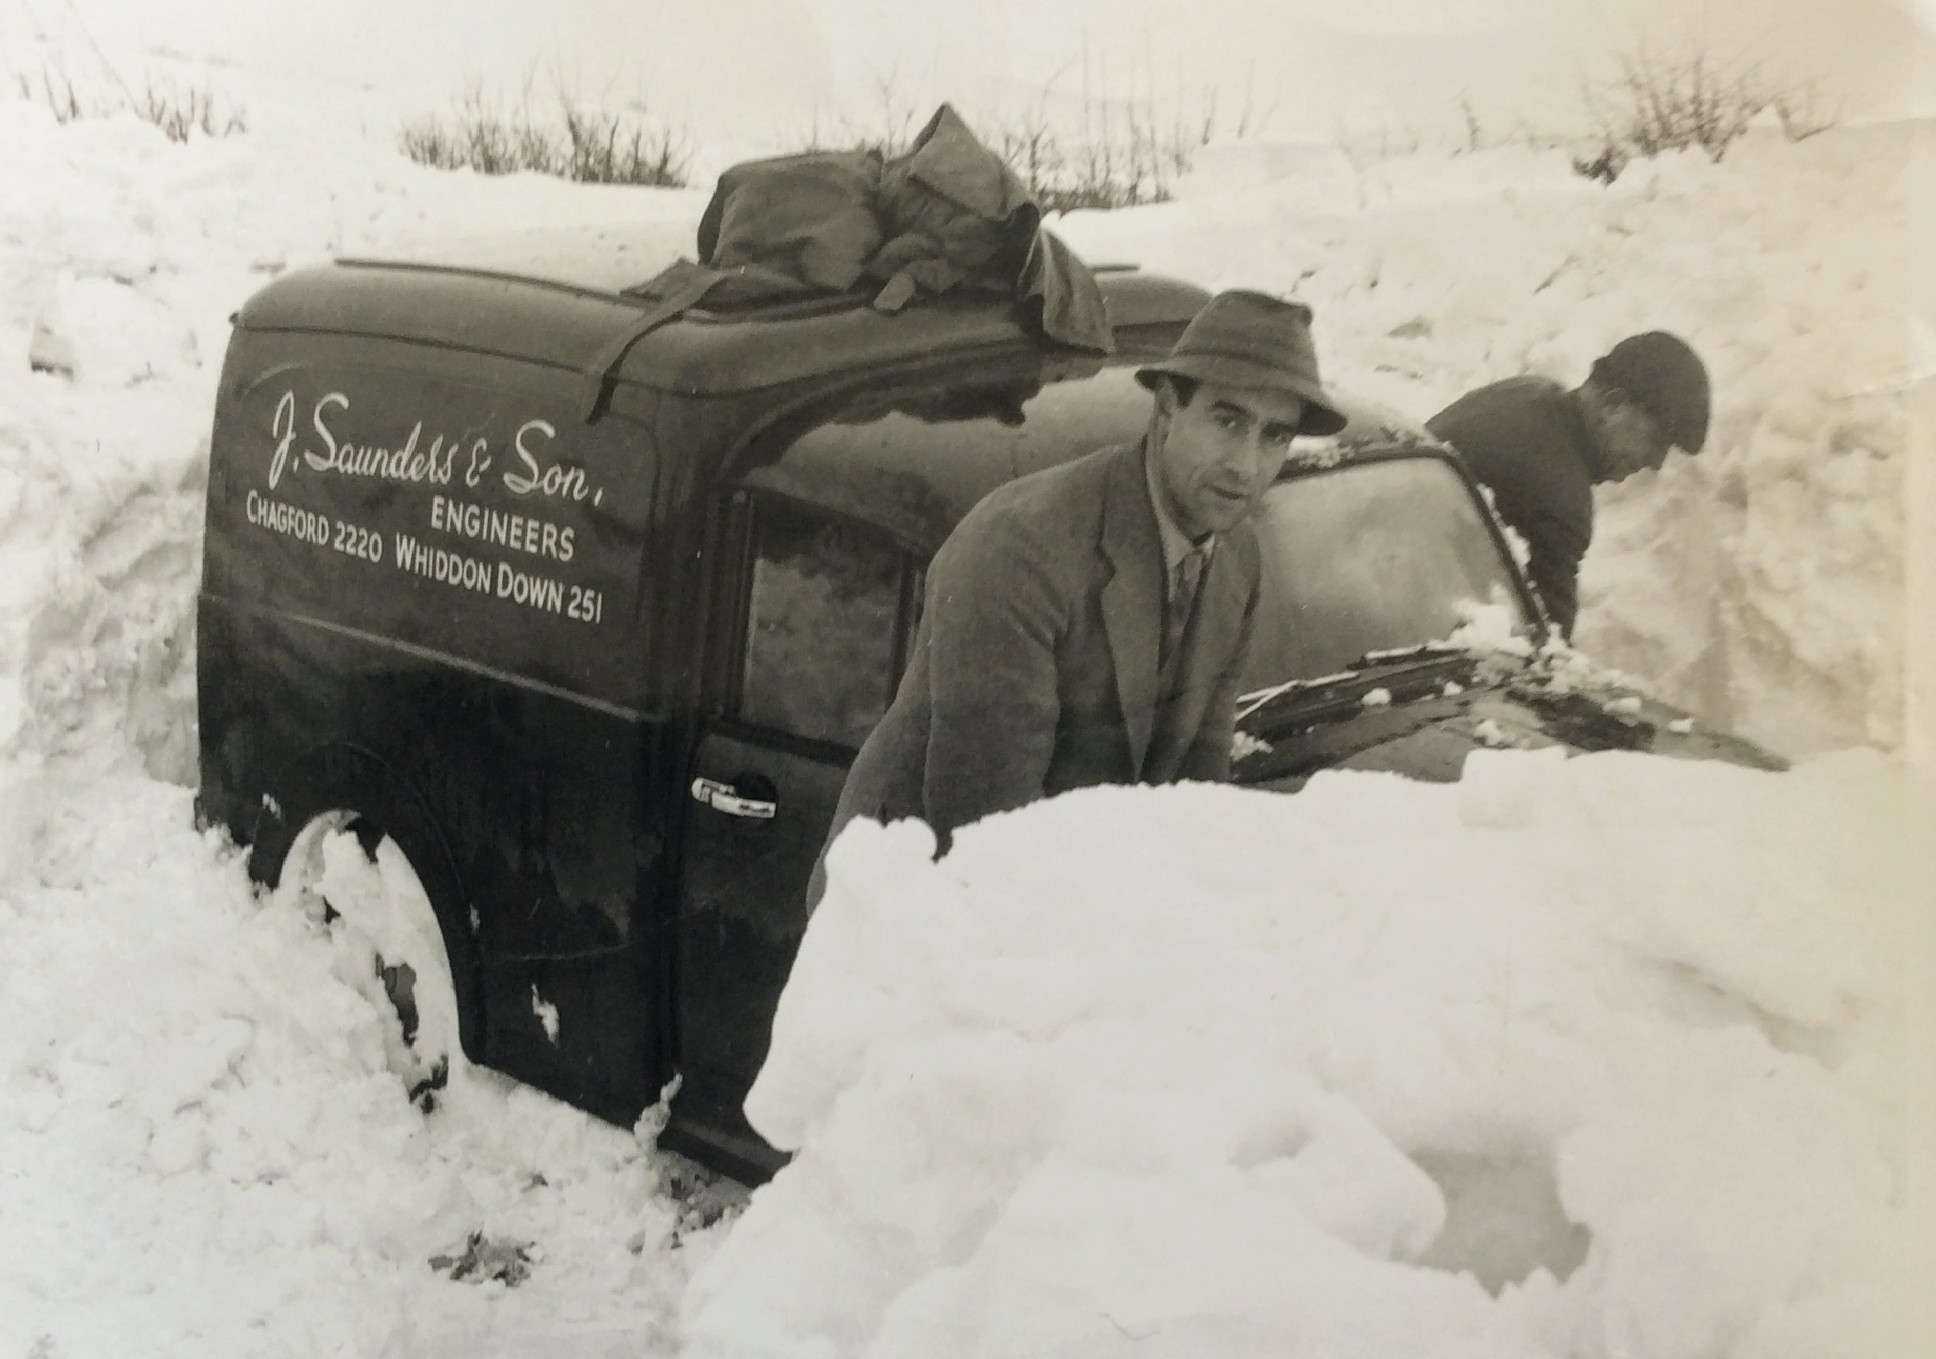
\includegraphics[width=.9\linewidth]{pictures/cropped/1963 blizzard outside the Post Inn.jpg}
  \caption*{The 1963 blizzard outside the Post Inn}
\end{figure}

\begin{figure}
  \centering
  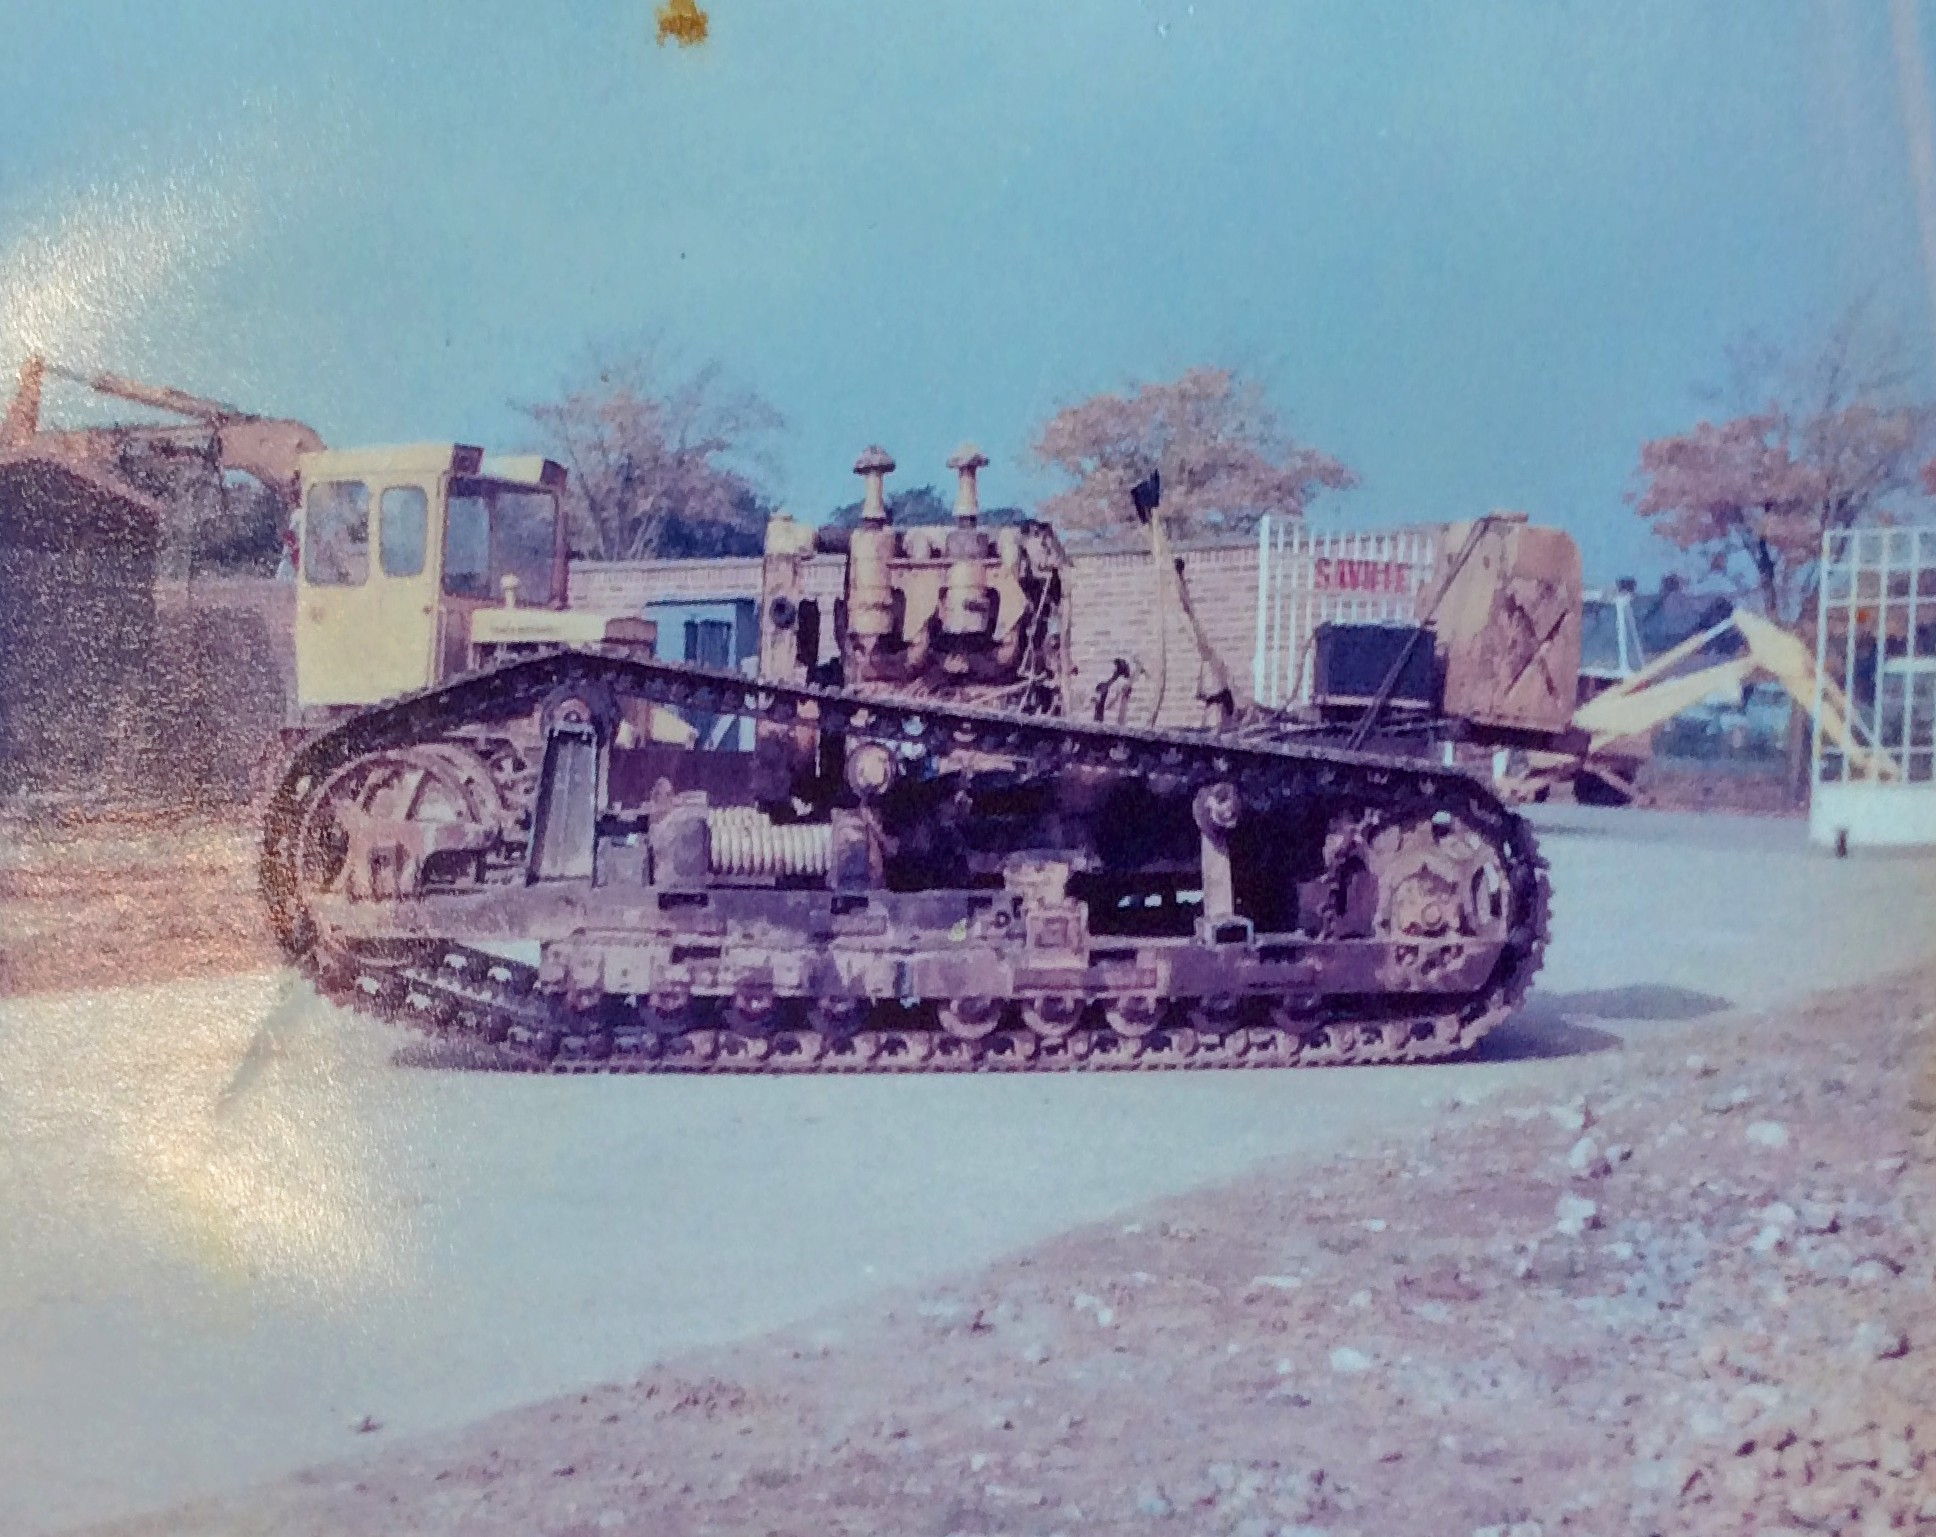
\includegraphics[width=.9\linewidth]{pictures/cropped/Fiat tank running gear.jpg}
  \caption*{Fiat tank running gear}
\end{figure}

\begin{figure}
  \centering
  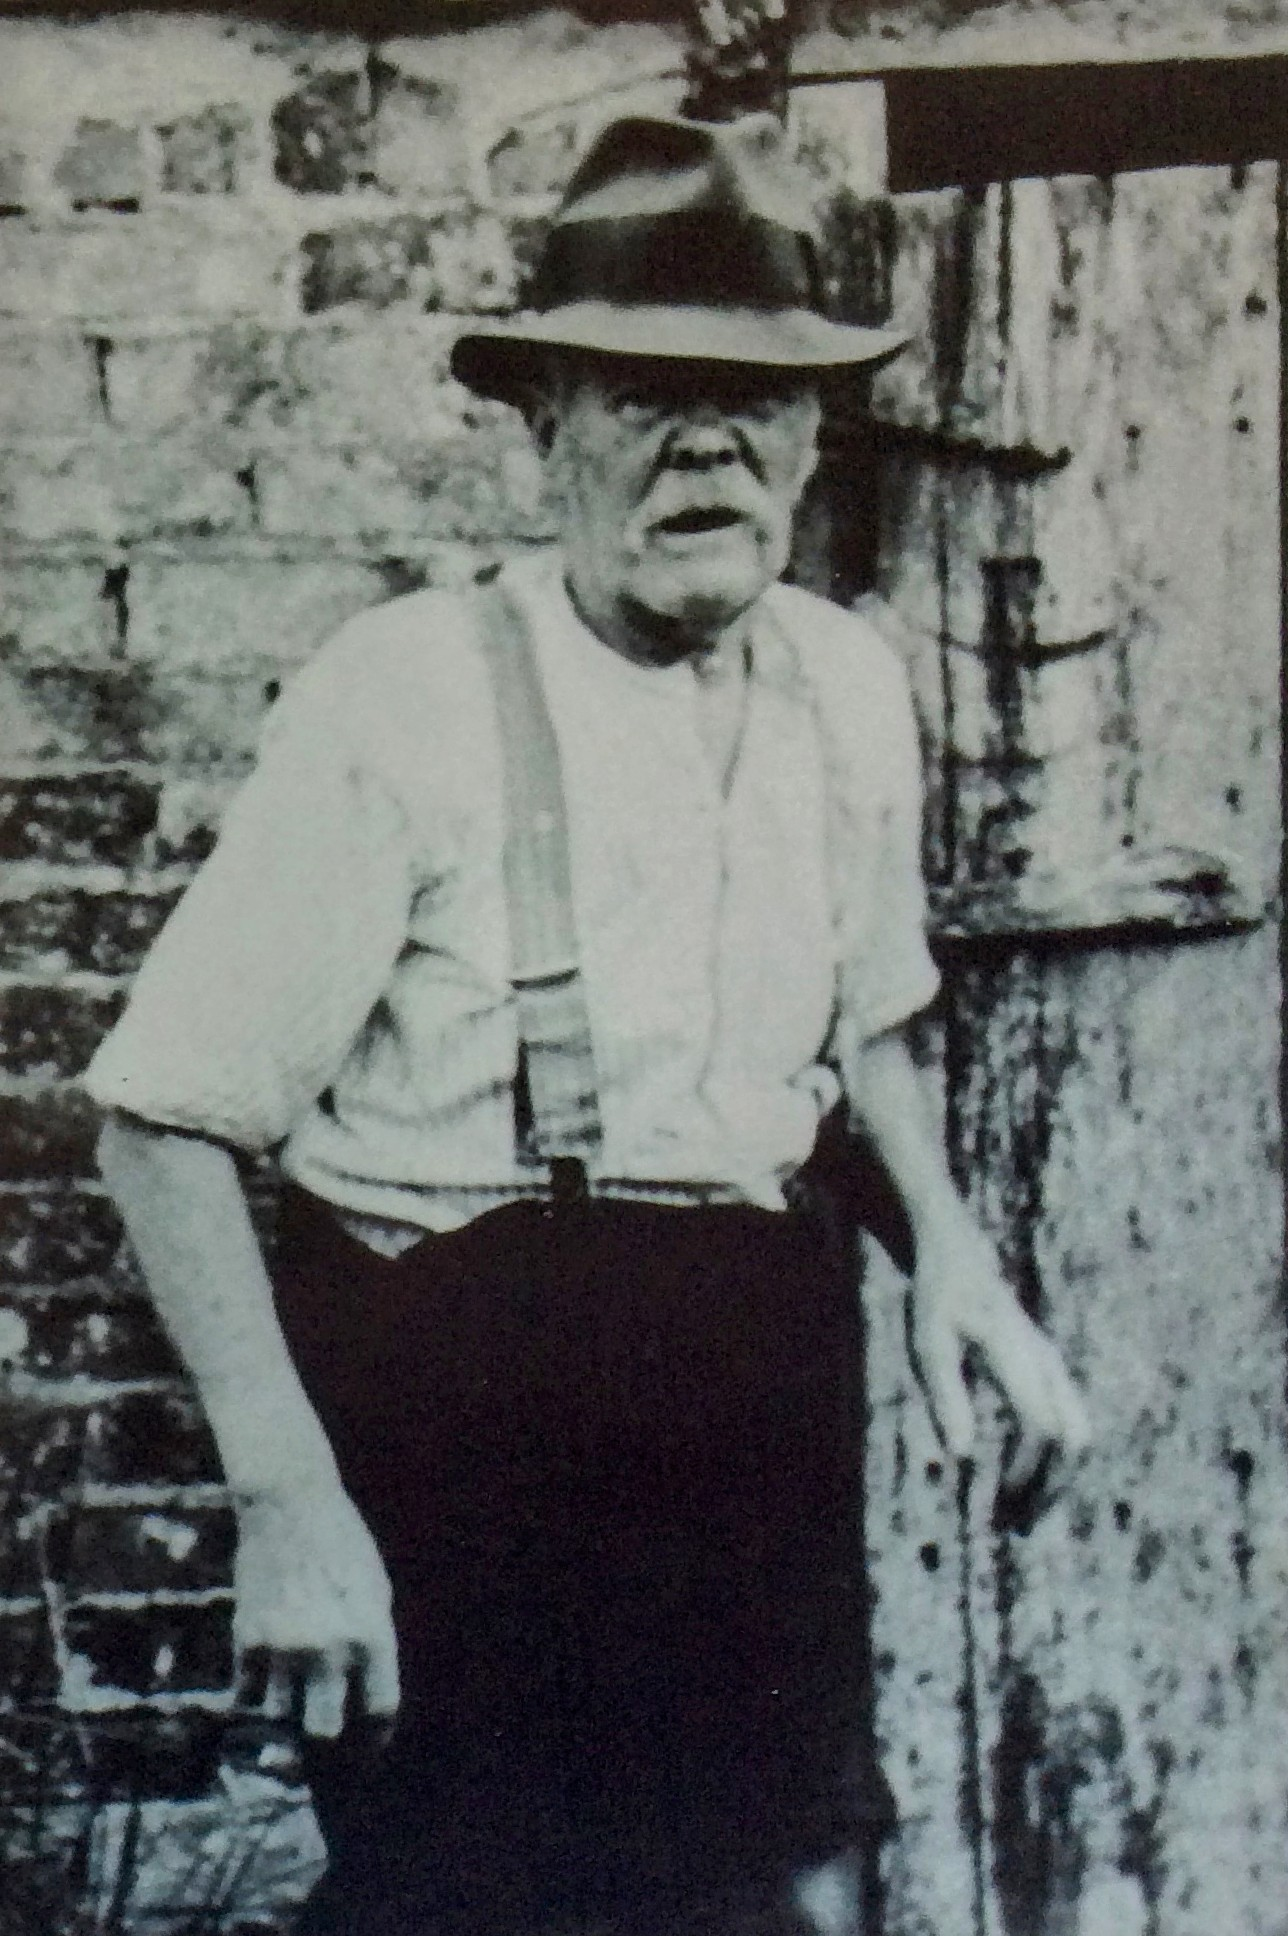
\includegraphics[width=.9\linewidth]{pictures/cropped/John Preston Butt.jpg}
  \caption*{John Preston Butt}
\end{figure}

\begin{figure}
  \centering
  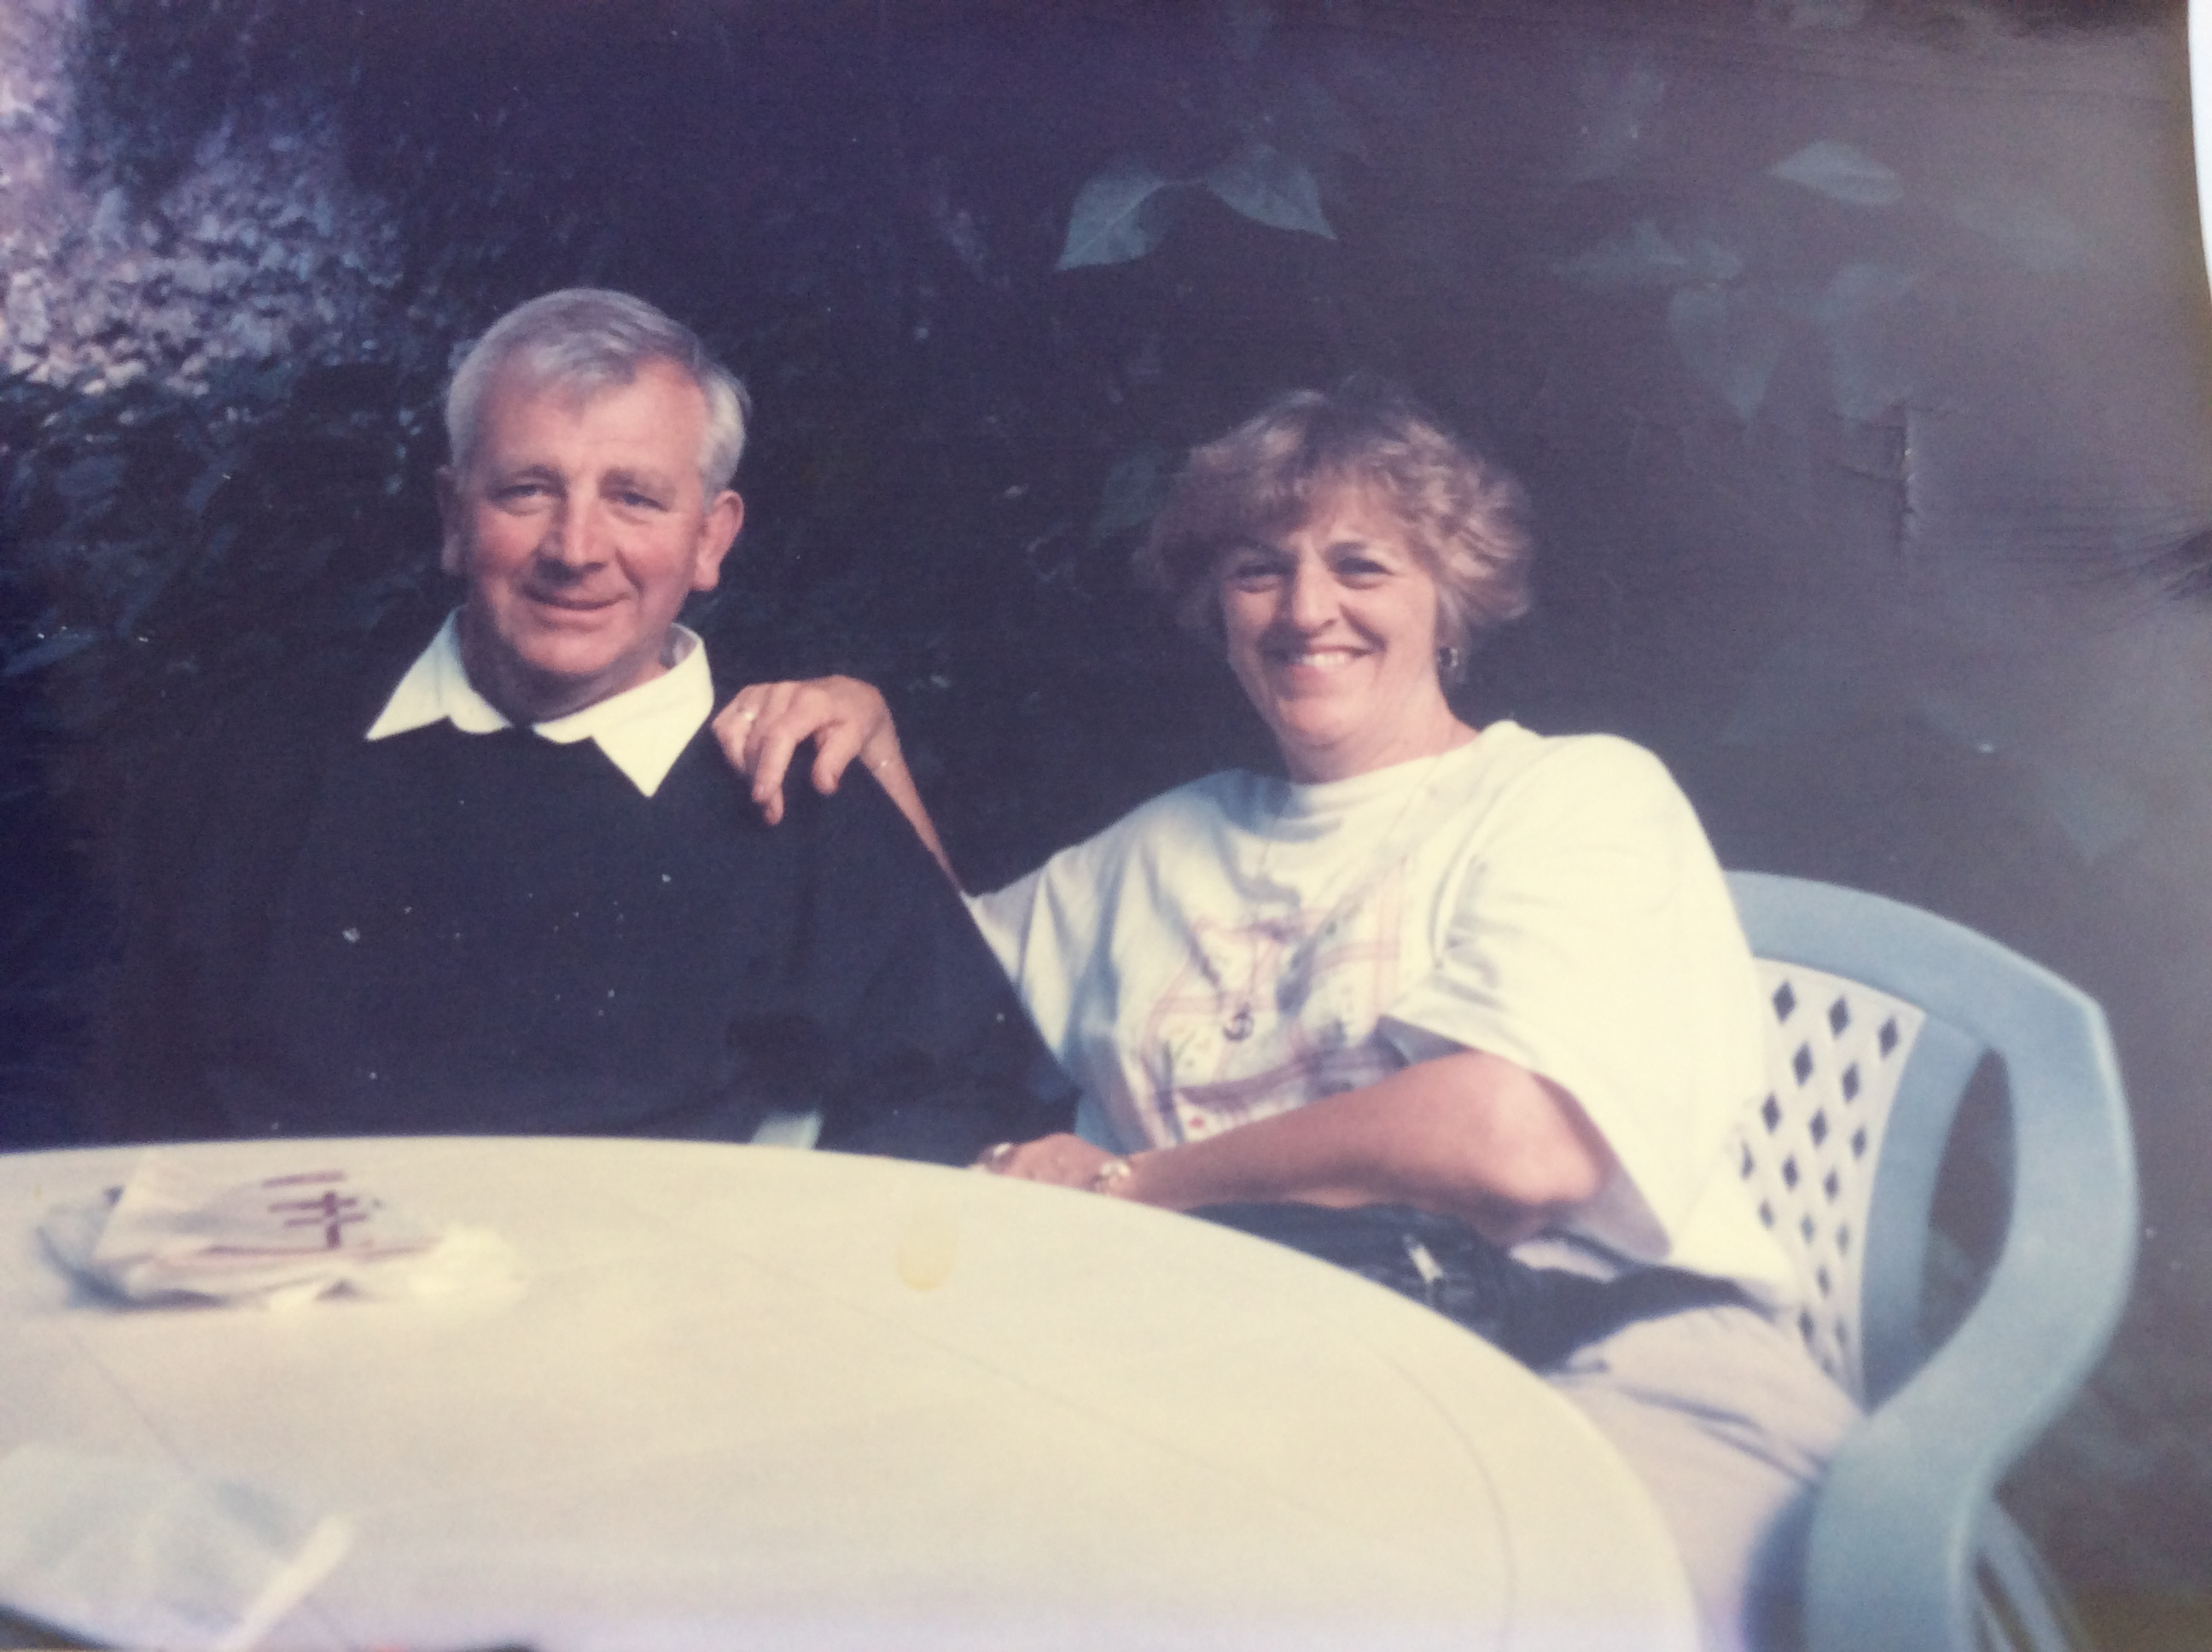
\includegraphics[width=.9\linewidth]{pictures/cropped/Mike and Vera.jpg}
  \caption*{Mike and Vera}
\end{figure}

\begin{figure}
  \centering
  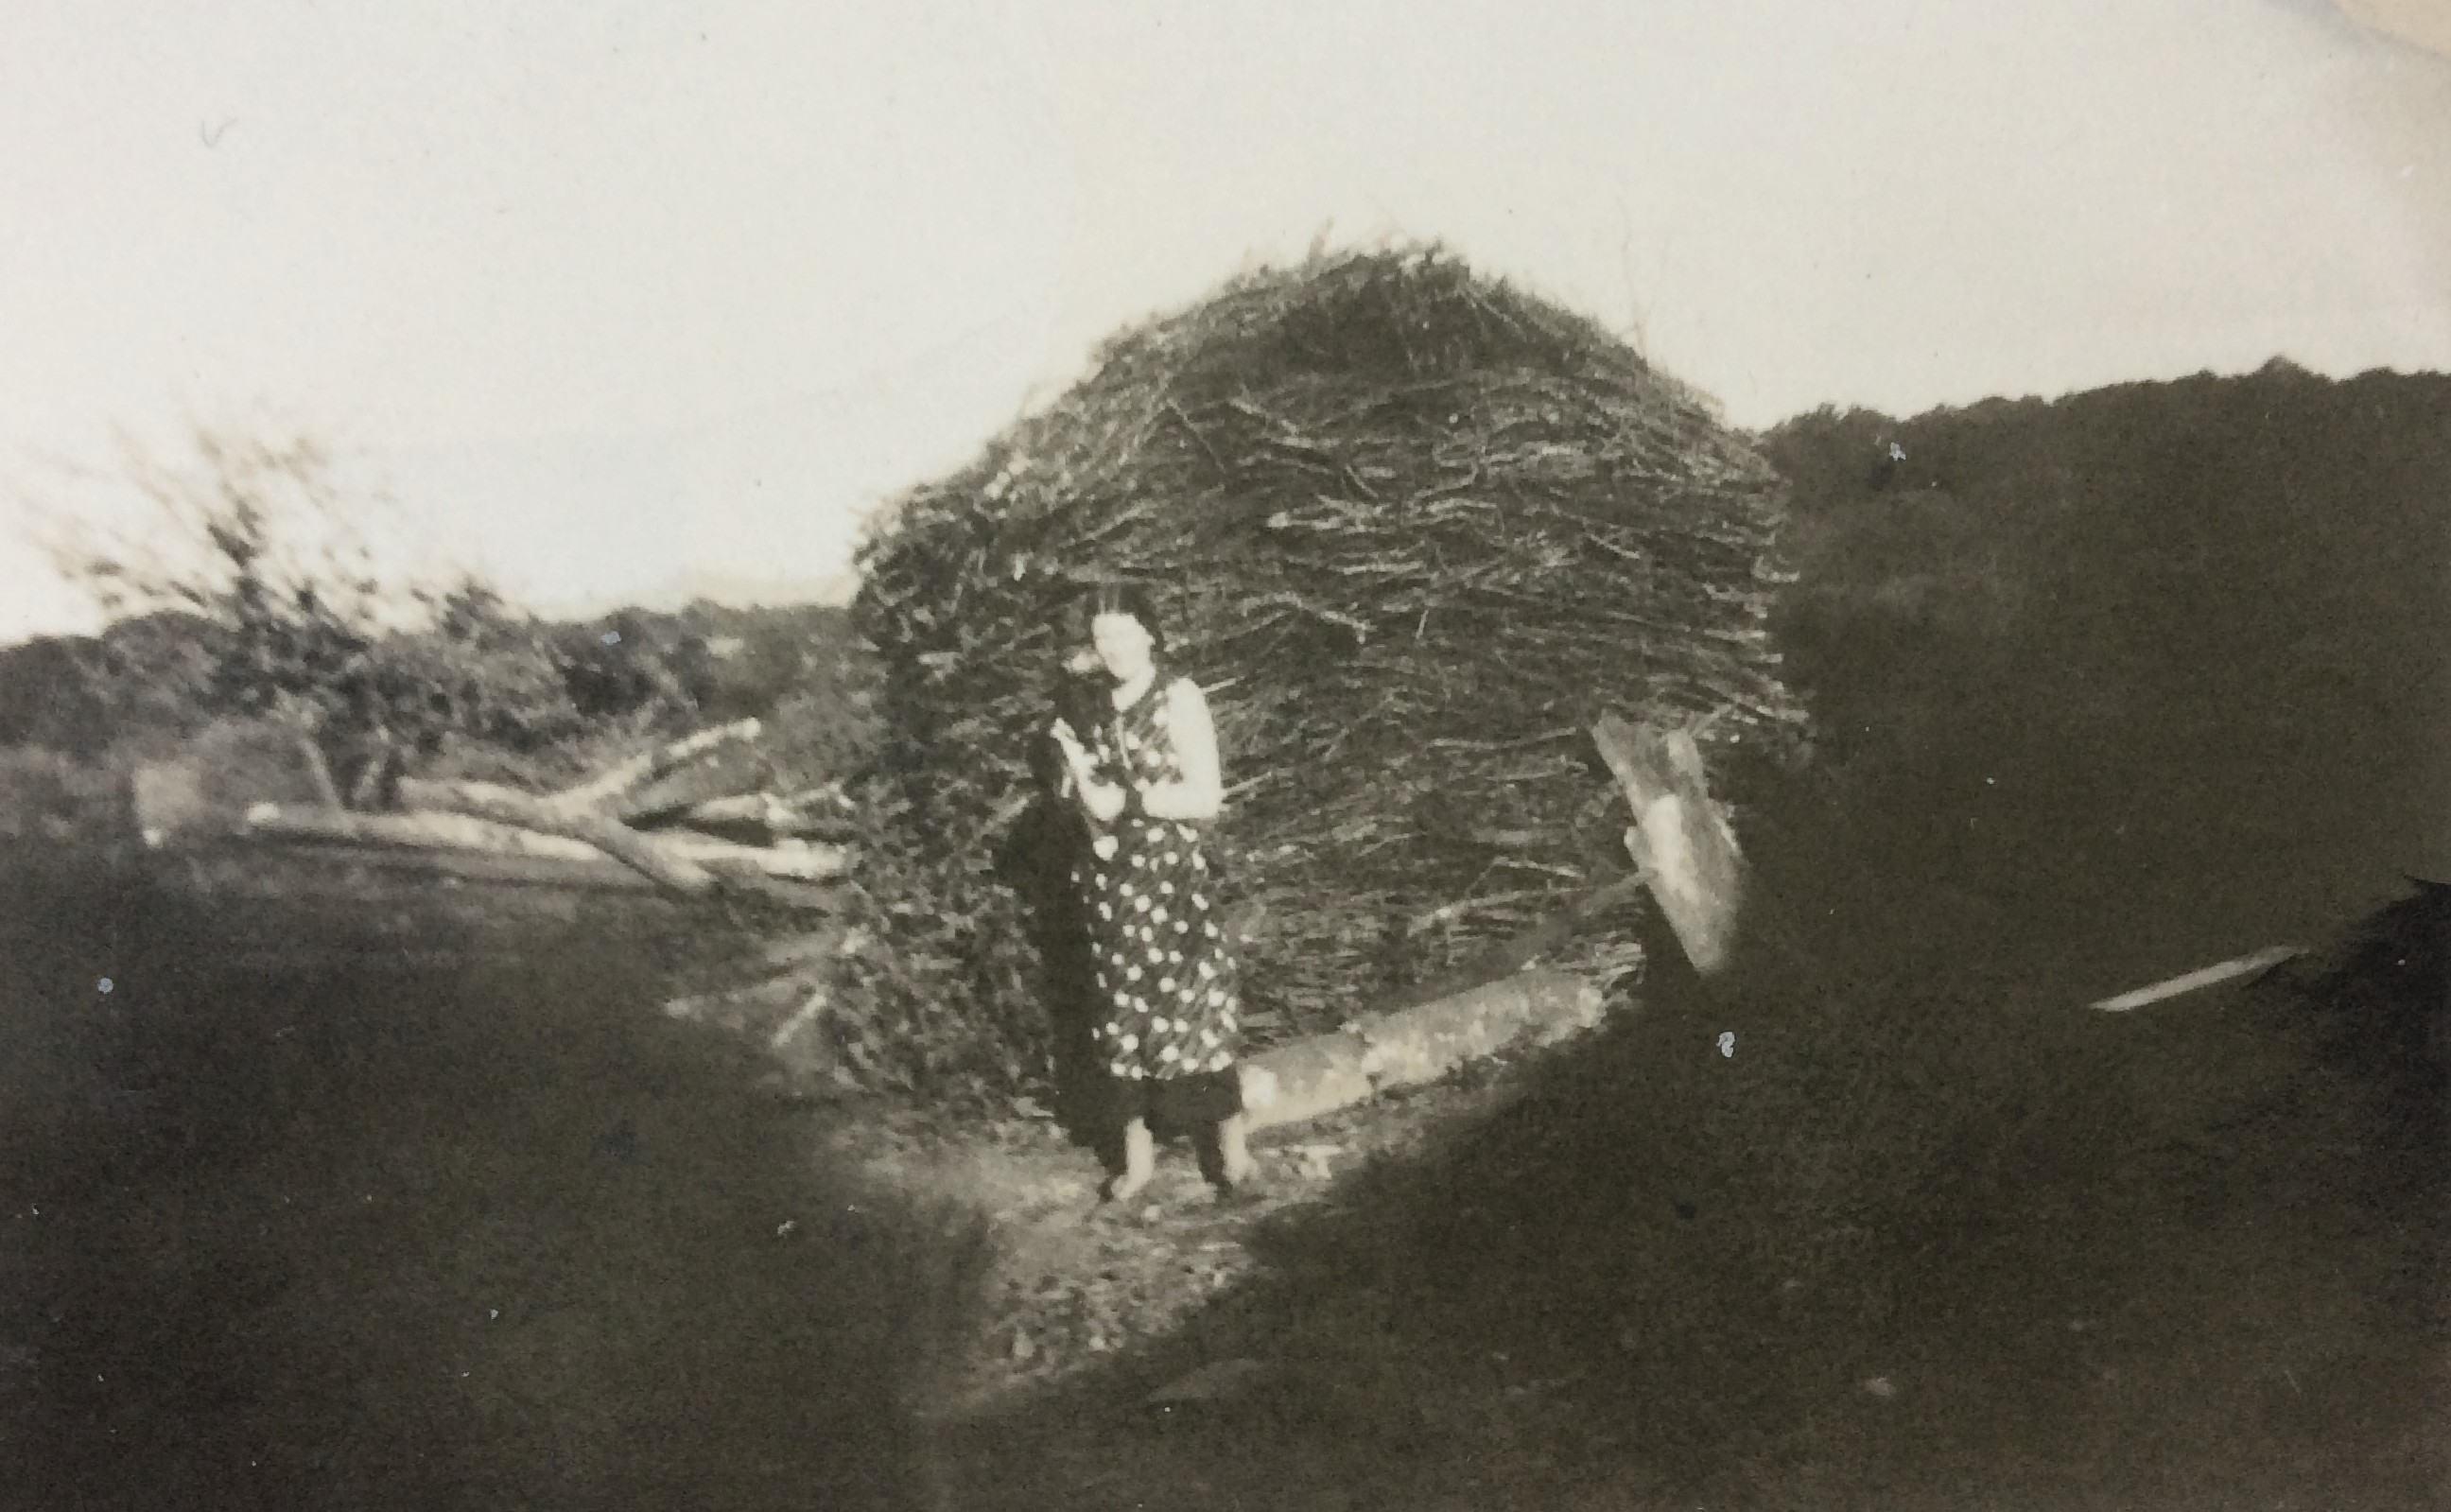
\includegraphics[width=.9\linewidth]{pictures/cropped/Mother beside a wood rick.jpg}
  \caption*{Mother beside a wood rick}
\end{figure}

\begin{figure}
  \centering
  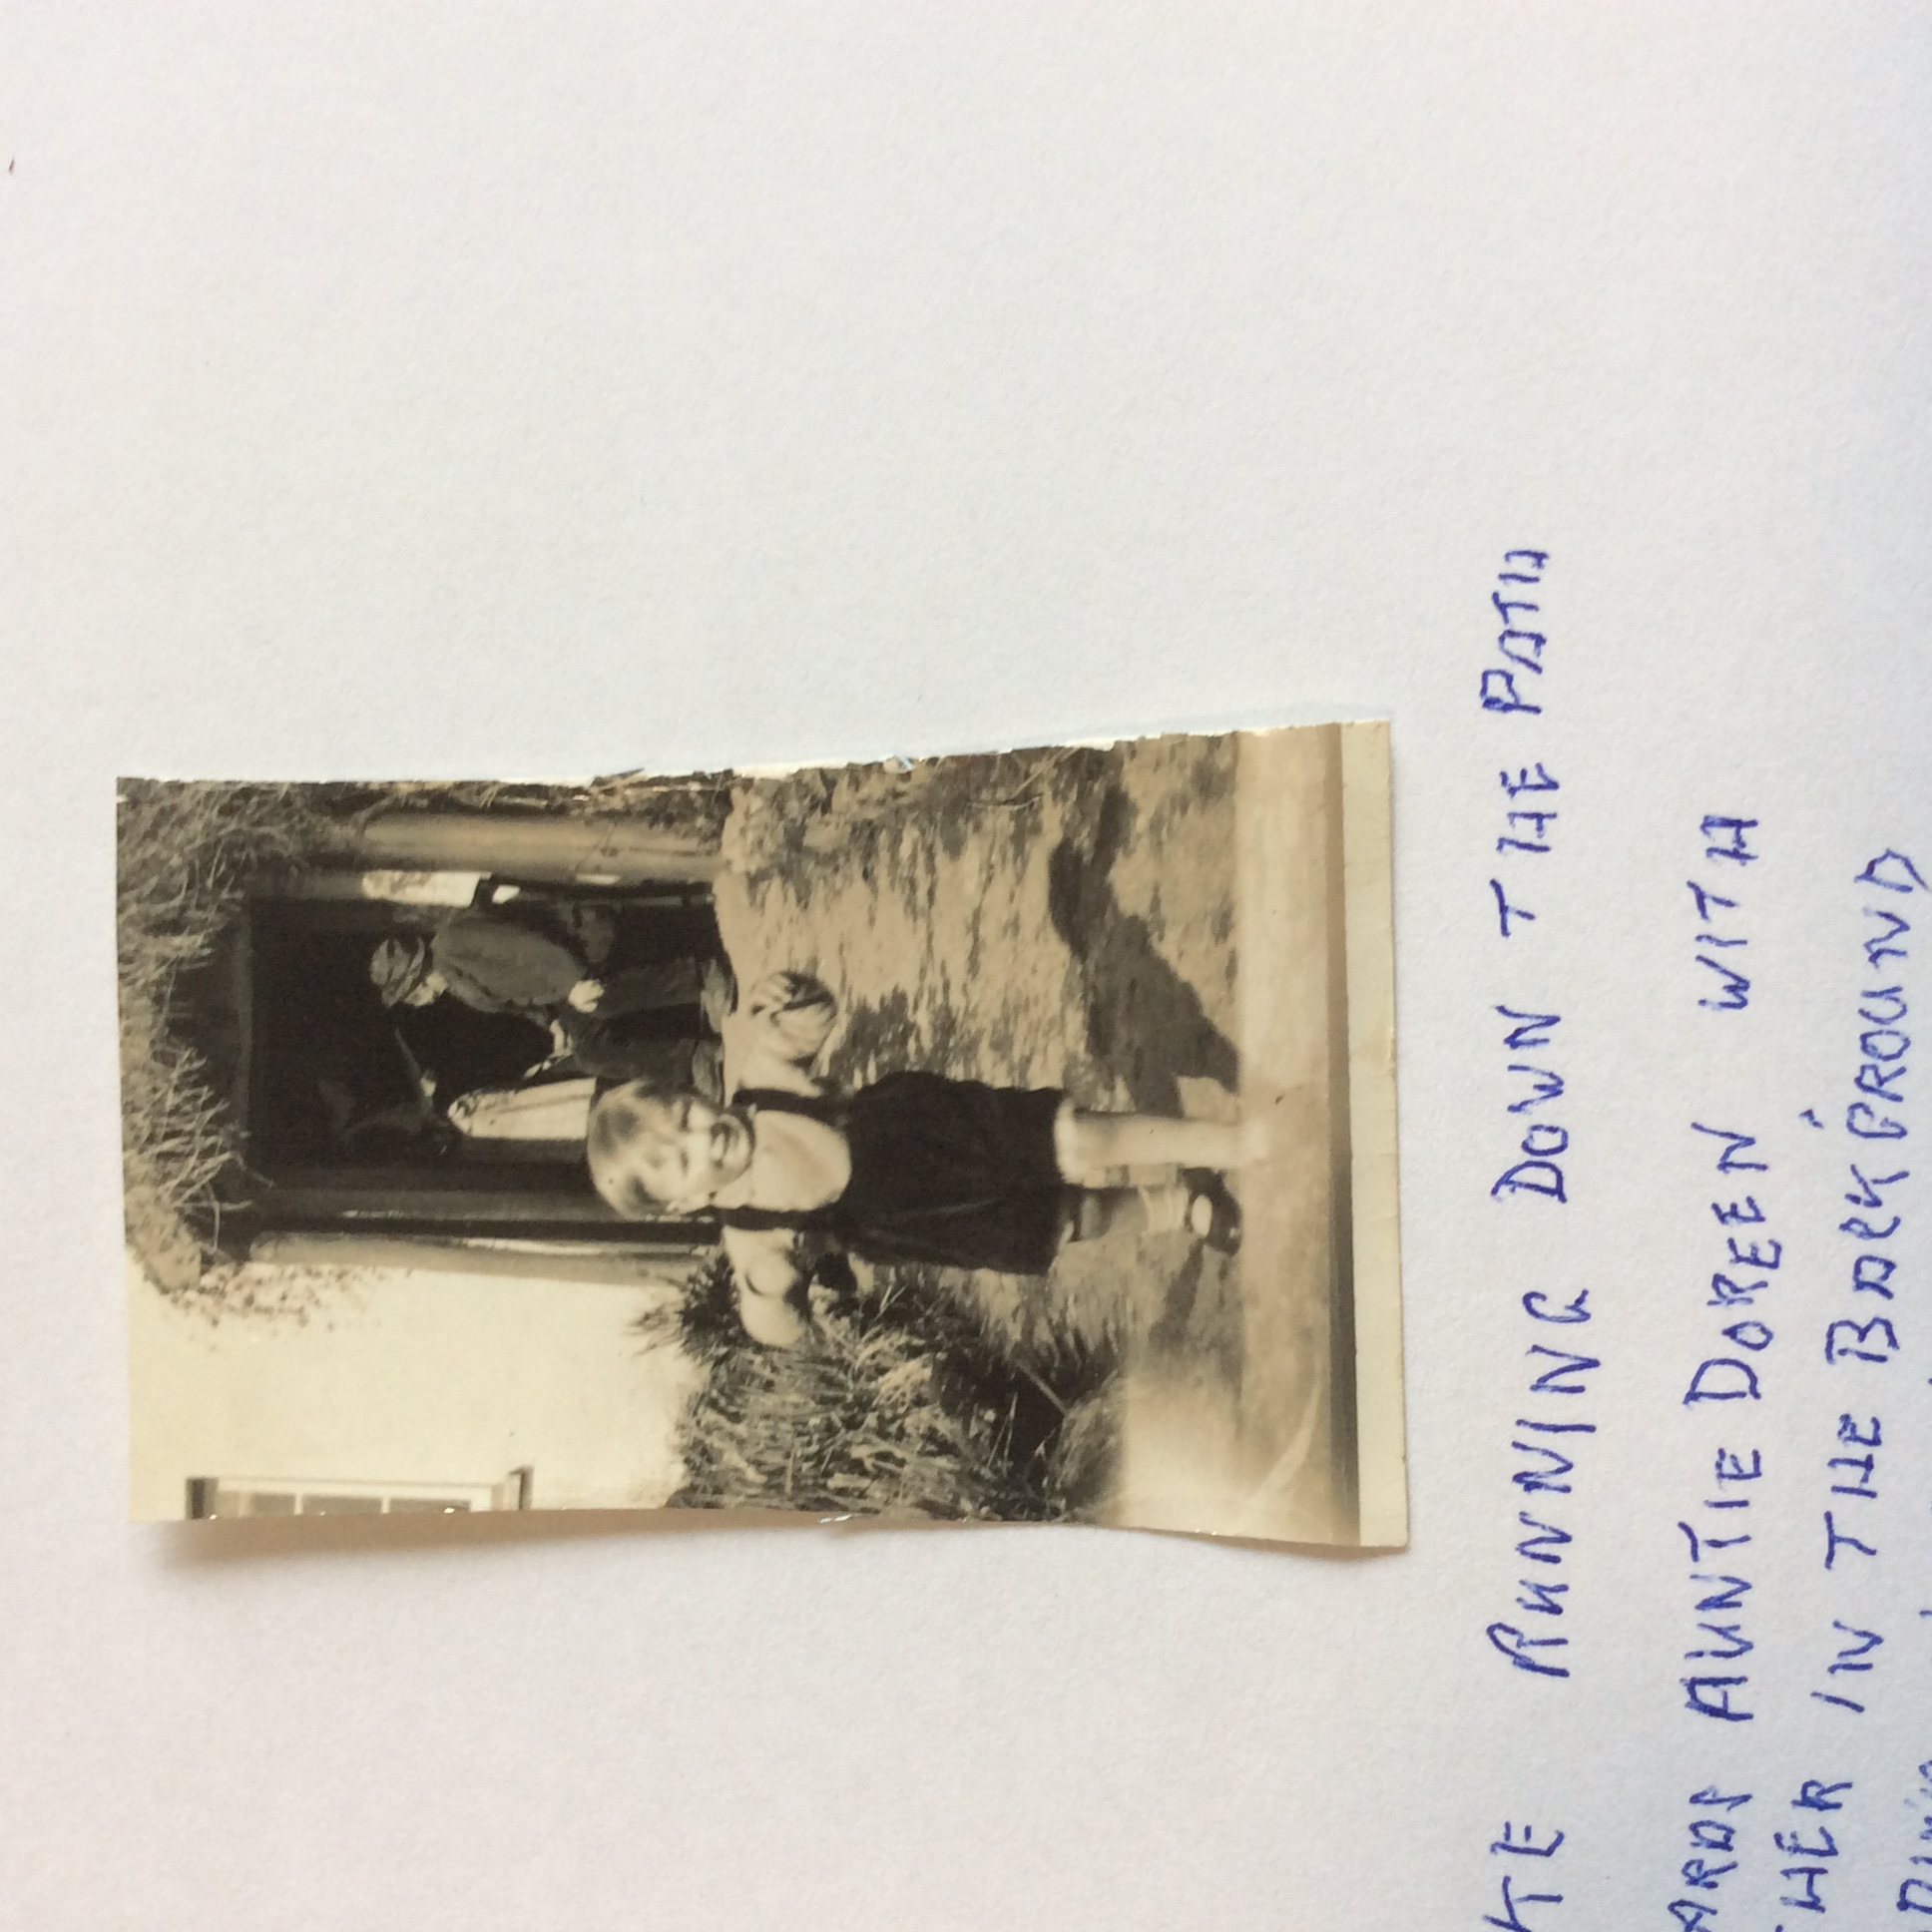
\includegraphics[width=.9\linewidth]{pictures/cropped/Mike running down the path whilst Mother is reading War news to John Preston Butt.jpg}
  \caption*{Mike running down the path whilst Mother reads war news to John Preston Butt}
\end{figure}

\begin{figure}
  \centering
  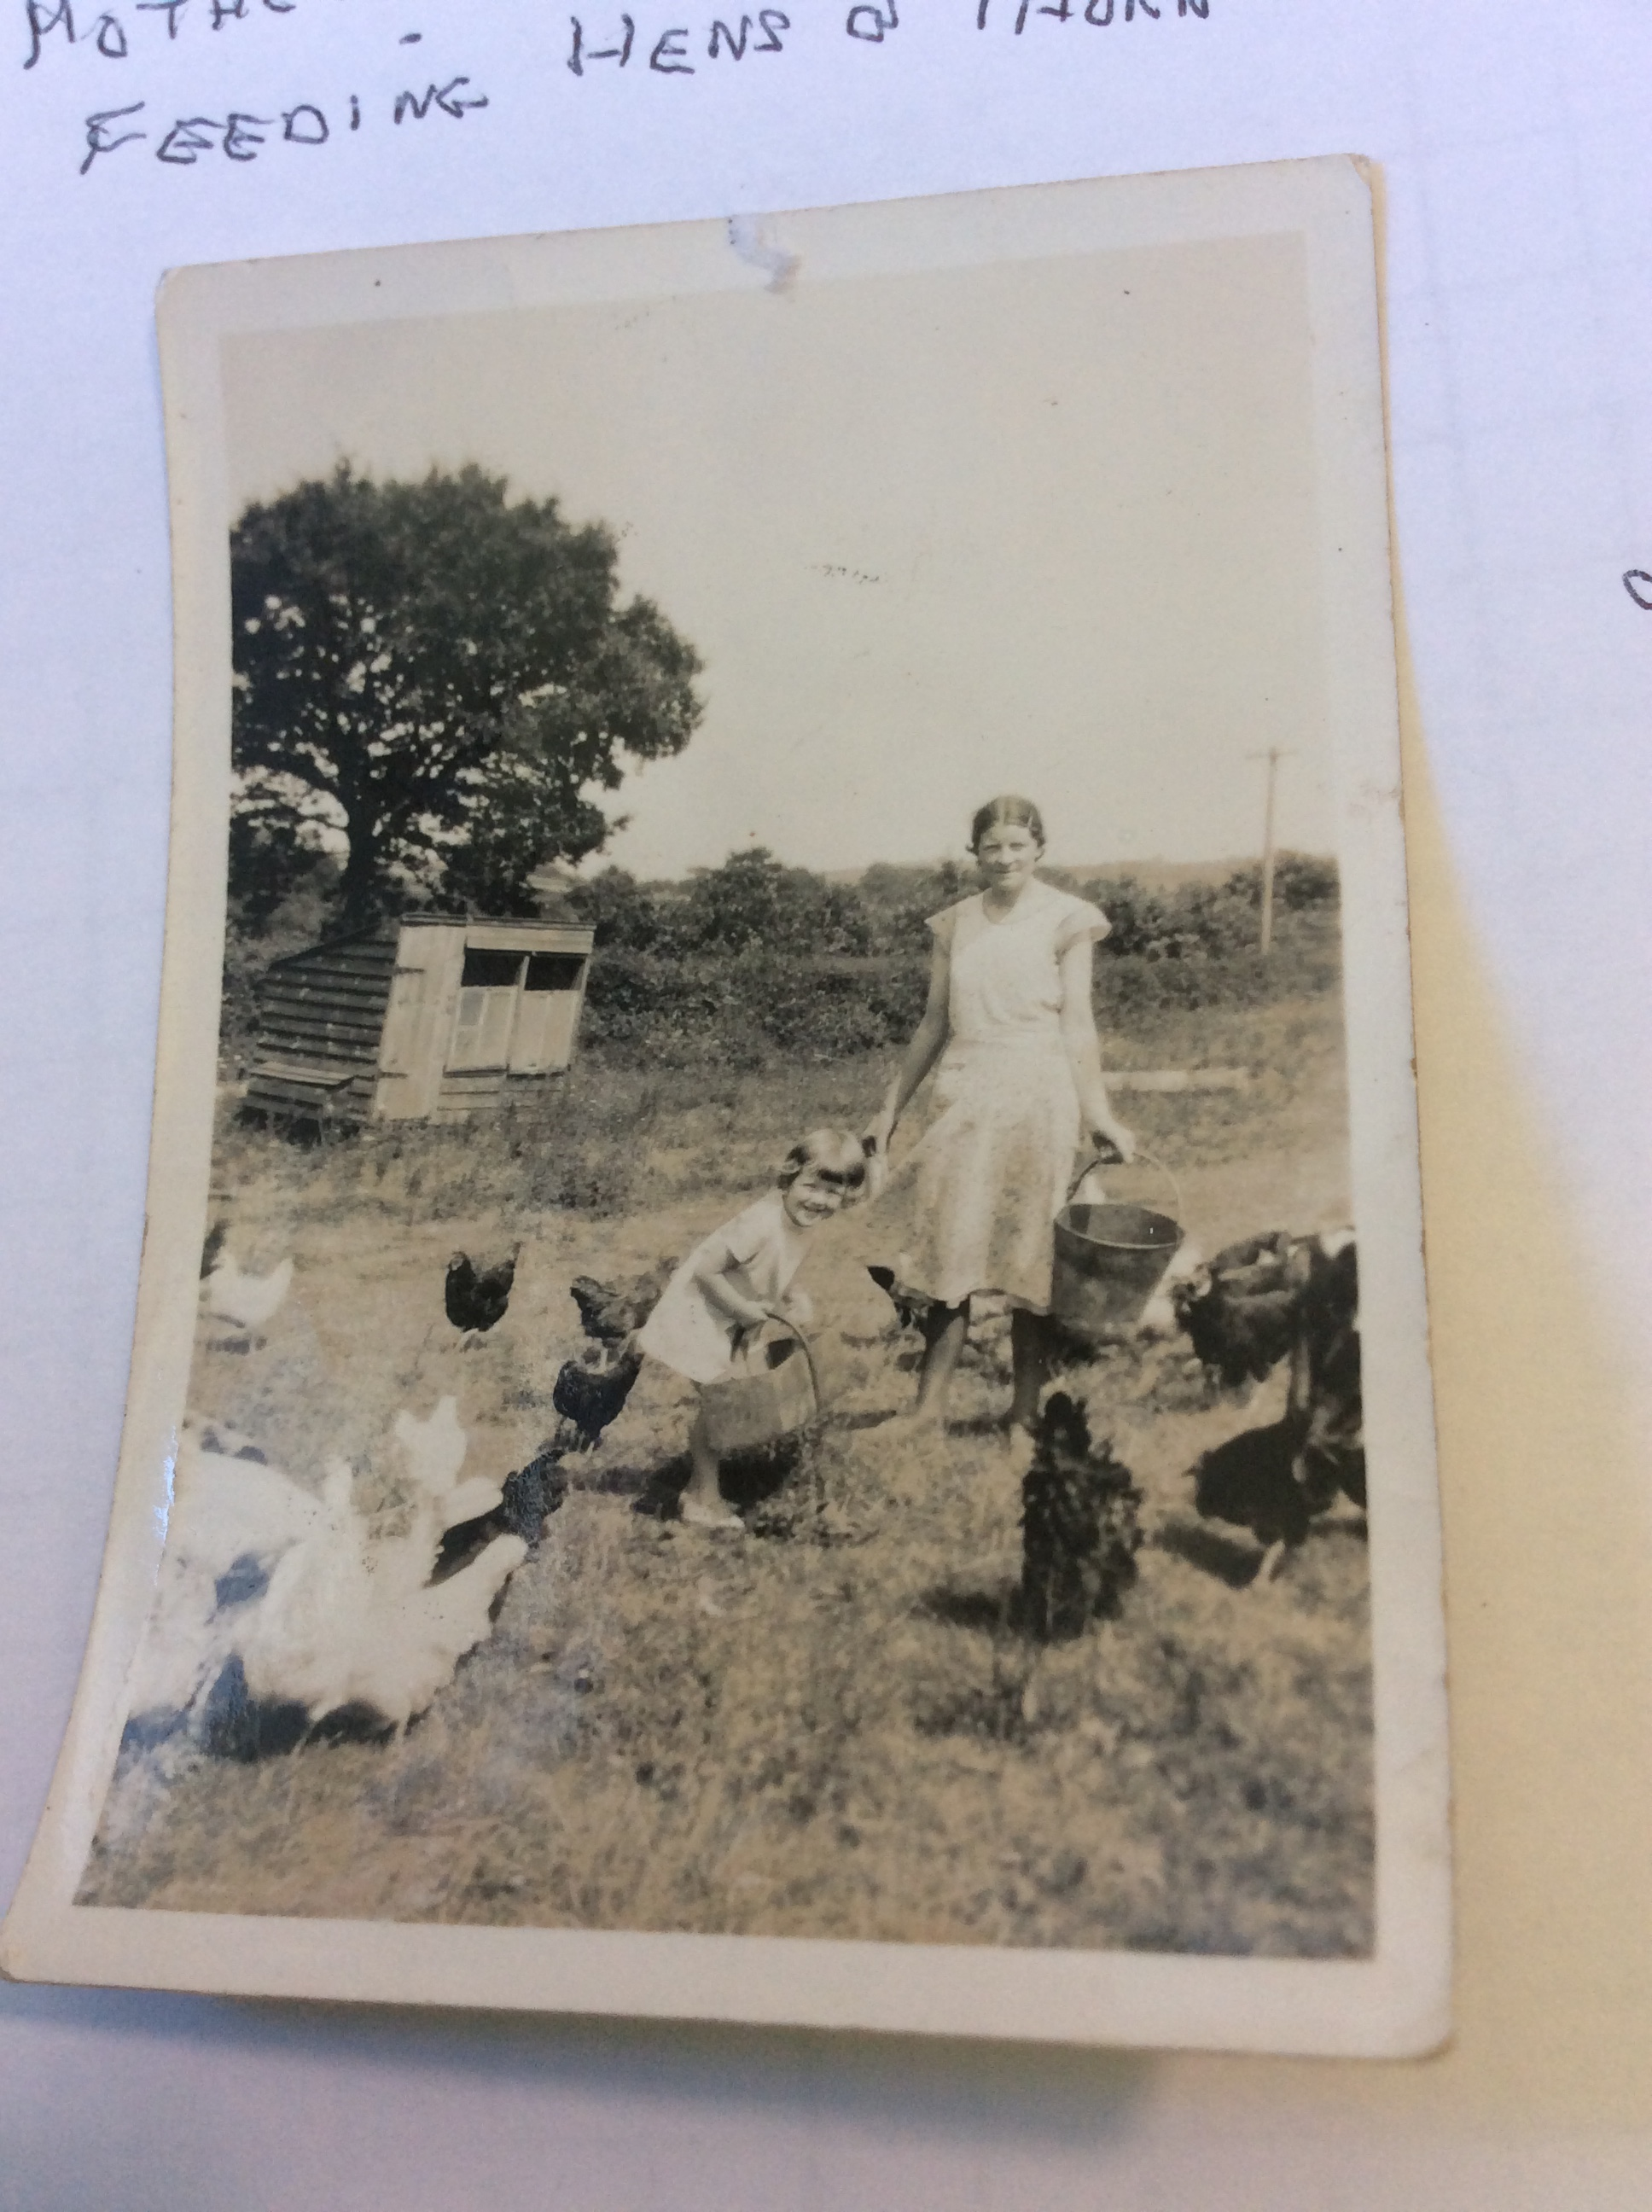
\includegraphics[width=.9\linewidth]{pictures/cropped/Mother with Cousin June.jpg}
  \caption*{Mother with Cousin June}
\end{figure}

\begin{figure}
  \centering
  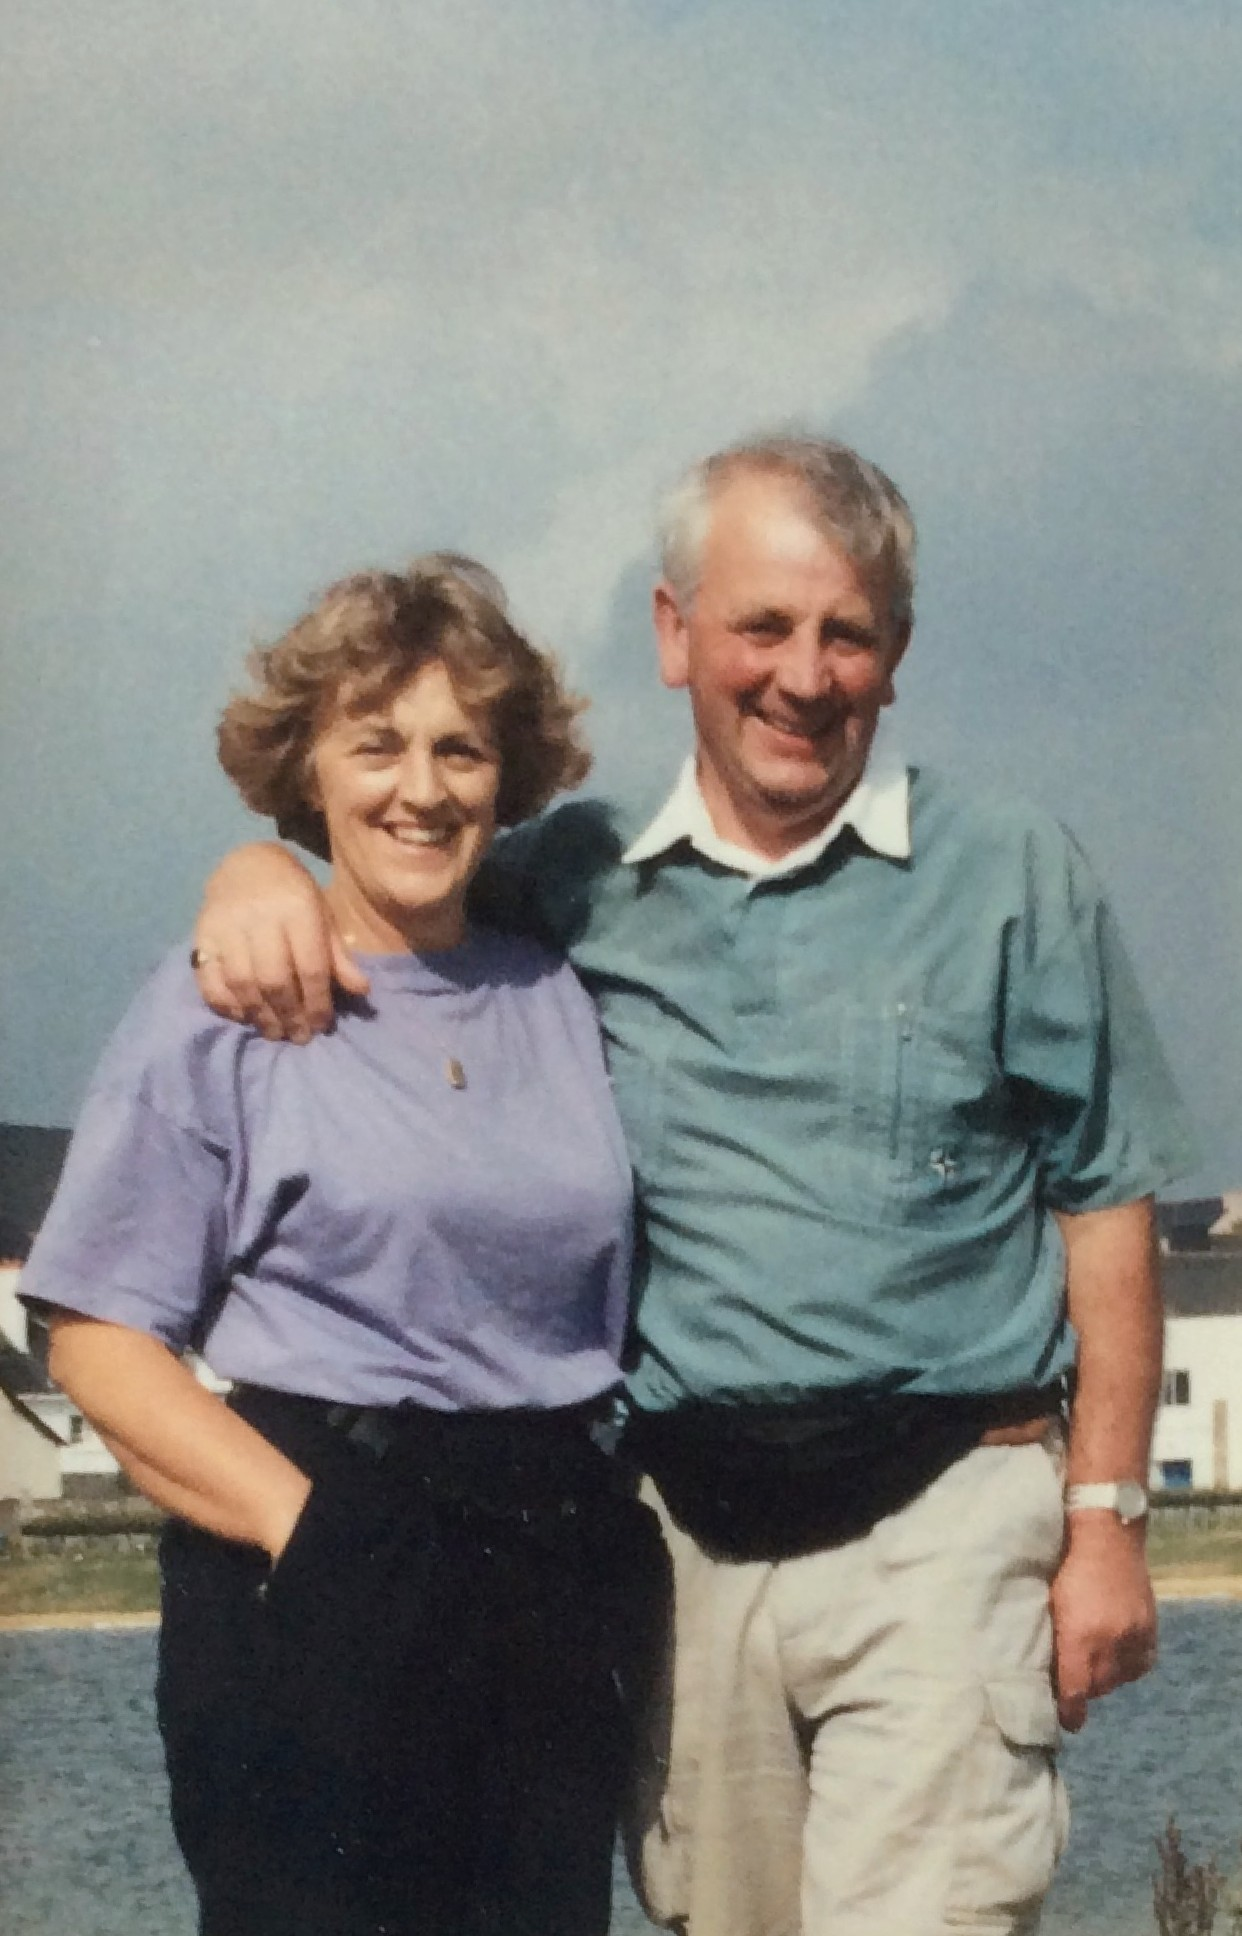
\includegraphics[width=.9\linewidth]{pictures/cropped/Vera and Mike in France.jpg}
  \caption*{Vera and Mike in France}
\end{figure}


\chapter{}
%!TEX root = ../thorn-moor.tex

I have always been active in my garage and as life has taken a turn have been
given a 1937 metal lathe with multiple speed pulley drives and a belt. I have
dismantled this system and have converted a 3 phase motor to interphase with a
multi speed computer system thus eliminating the multiple pulley system. I
turned away from engines and gears and made staves wooden and brass fittings
for banners all used for parades in Plymouth. I have taught myself leather work
and made sword belts and frogs for parades. I have often wondered when sewing
up a thatcher's hook pouch using the saddle stitch if I had learned this trade
and followed the occupation and become a leather worker would I be content in
my peaceful workshop or would I yearn for something more active as I did at
Thorn Moor in my early days?

Exeter Workshop --- Work from out of the blue! The phone rang one morning,
``Charlie Mann here. Wonder if you could journey down to me this morning. I
have a job I think you could manage to overcome for me.'' Charlie's company
over the years had grasped every opportunity as presented and found themselves
in demand for supplying the film industry with actual mock ups of military
vehicles. It transpires that Colonel Gaddafi of Libya was financing a film with
the title `Lion of the Desert' involving the factual history of when Italy
invaded Lybia in the 1920s to attempt to increase the expansion of the Roman
Empire and Gaddafi's own popularity in the world as at that stage it was at an
all time low due to the disastrous crime of the Lockerby airline bombing. The
problem in front of us is that the film required some military tanks Fiat 2 man
type. A mock up had been made from a Land Rover but failed as the wheels had
sunk in the desert sand. This time it is hoped I could recreate the Fiat tank
as near to the real thing as possible by using a bulldozer. This I did by using
an International 125 track loader from our sale stock and removed all existing
items such as the Operator's cab and load frames. I redesigned the track layout
by extending the length, raising the idler to match up with the profile of the
only copy plans available from Bovington Tank Museum. The tests were so
satisfactory that we finally manufactured six. These were shipped to Libya for
filming. They are found if you go into Google, type in Lion of the Desert and
scroll down the pages until you find `military vehicle'. Designing the
bulldozer to replicate a Fiat tank was a very hairy affair as Charlie Mann's
group of very serious faced men and Charlie sitting at a table in a portacabin
they passed to me a photocopy pages of the profile of the Fiat tank. One
question from them ``Can you make one like this?'' I was sitting stunned
looking at nothing, my mind running wild trying to create the minds eye view of
the modifications required --- 15 minutes thinking time. My response was, ``We
will do this for you''. All stood up and shook hands, in cars and home to
Exeter. We selected an International 125 from the used sales fleet. There were
no complicated drawings made to scale. I just made free hand drawings as they
came into my head. We conducted a completely different discipline of this
operation. All regular and day to day workshop repairs were carried out to 5
o'clock. Then all stopped, had a break and something to eat thus ensuring we
returned to the project with a completely changed mindset. All bulldozer
equipment set was removed on the yard workshop floor, washed with hot water and
detergent with the machine positioned and all recreations marked and drawn out
by chalk on the floor. My boys responded to the challenge in top shelf manner
and by the end of the week of evening work there was a military power unit. The
film company representative came and gave it a full test resulting in a fully
satisfactory pass and immediately ordered a further five modified units.

My Uncle Ronald once said, ``The trouble with folks moving down to Devon is that
they think we Devonians are daft because we have no sense!''. How true as when
I was a young man I set out with one aim in view to finish the project only to
find that a journey down the other road would have achieved a better result ---
a fault that holds fast in future years. I decided to build a double seated
canoe using plans from a practical woodworking magazine. The length of the
designed vessel was 17' 6'' to be built in my garage in a very cold winter
season so fault 1. I cut the length from 17' 6'' to 17' to accommodate the
project in the garage enabling the door to close and lock. Mistake 2. To
upgrade the marine ply from 3mm to 4mm. The hull spares were increased in size.
On completion the vessel looked solid but when launched it immediately gave the
impression that things were heavier than required and the removal of the 6''
waterline length meant the hull sat lower in the water. Nevertheless my friend
and I entered into the Exeter Canoe Club race. Despite being left at the post
to start with after half an hour of paddling we began to catch the competitors
and overtook at regular intervals being very concerned that it was like pulling
a log through the water rather than a responsive vessel. We reached Double
Locks, turned and kept up our relentless paddling finally reaching the finish
at Exeter Basin. We were congratulated on achieving 2nd position in the touring
canoe section. Congratulations were quickly followed by reality as we wondered
if there were only 2 touring canoes! A further follow up from there is to never
look on one side only. Turn the coin over and look at the tails as well as the
heads --- that applies to every avenue of problems presented.

I started one day to collect an architect from Hilltop in Plymouth and visited a
generator unit that is powered in a Devon and Cornwall Police Hilltop Radio
station. My companion was named Tom Jane.   We knew each other well as we had
carried out many of such inspections so conversation was always great but a
happening occurred which affected both of us after we looked at the generator
and started our quite long descent to return. I was driving quite slowly so as
not to cause damage as the path was very deeply rutted with small loose
boulders. Looking in the distance I could see a spiralling cloud of dust moving
very fast. Tom's voice said in alarm, ``Better pull in here where there is a
wide area''. We stopped and waited. The drive was in another world as a van
passed. The energy from it was unforgettable. We remarked to each other that we
would not like to be on top of the hill when he gets there. Next morning Radio
Devon News mentioned that a person had committed suicide on Kit Hill and was
asking if anyone had any information to contact Lostwithial Police. I did give
full particulars of what we had seen. The response was, ``Goodness! You are
spot on. How did you report that information in such a short time?'' I told
them that the energy coming from that van was disturbing. I could not help but
see there was big trouble of some sort.

Whilst talking to the Police, let's talk of the policing of Thorn Moor, Cheriton
Bishop. The area policeman was a typical comic book build, tubby, red faced and
kindly man, named PC Tonkins who lived in the Police house at Tedburn St Mary
but to me a small boy was always in the right place of minor offences committed
by small boys. One day my friend did not have a bike so not wishing him to walk
I gave him a lift. We arrived with David sitting on my rear carrier. The shock
of seeing PC Tonkins cycling towards me caused me to lose control and run up a
very steep bank and fall backwards with the bike on top of both of us. PC
Tonkins stood in the road and exclaimed that that demonstrated the reason for
not riding 2 people on a bike. He waited to see if we were OK before continuing
his journey. Luckily it was outside of David's house and I continued to cycle
home. Sometimes we would see PC Tonkins ride past our gate on his way to his
favourite cider cellar and later in the day riding in a car with his bike on
the back having a very necessary lift home. Some years later PC Tonkins retired
and was replaced by a PC Cannon immediately renamed by the locals as ``bang
bang''. Big enquiries were made about his character. I wanted to know whether
or not he let minor deeds go unnoticed. I also wanted to find out whether he
enjoyed paperwork as if he did this would not be good as he would probably make
out a ticket for blowing our nose. One evening I was aged about 16 and was
walking quietly beside a hedge leading to a gate to the road. As I got to the
gate I checked again that the gun I was carrying was empty and left open. Prior
to opening the gate and stepping on to the road I was confronted by PC Cannon
or should I say Bang Bang. He had remained hidden until I stepped on to the
road. He greeted me with the following ``Let's see, your name is Michael?''
``Yes sir'', I replied. ``Let's see'' he said ``Is that a 12 bore shot gun?''
Again I replied, ``Yes sir. It needs a shot gun licence like this one'' I said
pulling the very item from my top pocket and handing it over. PC Cannon said.
``Ah yes. I thought you of all people would have one.'' I thought, I expect he
was hoping that I did not. I watched him read through the form and I thought
that he was a paper man so nothing out of place will go unnoticed so watch out
farmers in this area. A rumour circulated that this PC had been relieved after
the war as a prisoner of the Japanese Death Railway. I thought that if that was
the case, I would forgive him his general unforgiving conduct.

Some years later my friend George Gillard and I were asked by PC Alan Parsley of
Whiddon Down if we would become Special Constables to support him with traffic
or, as happened at the time, check points following convicts' escape from
Dartmoor Prison. This we both did and spent many winter nights having training
at Moretonhampstead Town Hall. One evening when a member arrived late he told
us that President Kennedy had been assassinated. We all stood in disbelief. I
was called to help a regular Constable with a road check at Beter Cross on
Dartmoor commencing at 7 pm until midnight. We sat in my car as the night grew
cold with heavy fog due so we could hear a car from miles away and would get
out of the car standing on each side of the road and wave our torches at the
car to stop. Some would not wish to stop as our torch lights would reveal their
passenger to be someone other than his wife. Not our care so we thanked them
for stopping and waved them on their way. In the late 1950s I was led to
understand convicts would escape to pay back a debt to the tobacco baron and
the longer they could stay out and cause disruption the more the debt was
reduced.

\chapter{}
%!TEX root = ../thorn-moor.tex

Dear old Farmer Palmer, as seen through the eyes of a young boy of my age, was
short, portly, and so innocent that the reality of life must have mercifully
passed him by. He passed on his various encounters to second and third parties
which were received with goodwill and mirth. Having seen the special tractor
that Worthy Anstee had built for himself, Farmer Palmer requested that Worthy
build a similar unit for him which was duly done and the day came for a test
and customer approval which was received. The tractor was duly delivered and
with Worthy in the driving seat Farmer Palmer was pleased sitting beside him.
The tractor was driven at top speed to show off its capabilities. The speed
frightened Farmer Palmer who not wishing to offend exclaimed ``slow down. Tis
fast enough for cutting corn.'' In the early days of the bombing of Exeter
Farmer Palmer stopped his car beside our main gate. After the normal greeting
to my father he said, ``Quite a heavy night of bombs''. ``I said to my wife
hail up. You yerd the Germans are coming''. So we lifted our main sheets over
heads and settled down underneath. The local garage had an urgent call from
Farmer Palmer saying ``Will you come quick as our old car is alive. Every time
me son-in-law, Jack, turns the starting handle to drive the car it keeps
walking towards him and has pinned him up against the wall so would you come
and rescue him''.

When I retrace my memory back to my age of 10 years I become aware of how much
we as individuals manufactured for ourselves. It started by me sitting on a log
in the orchard watching Dad make me a whistle from a willow branch using his
penknife. A few days later found me sitting on the same log making a whistle
with my penknife --- every country boy would own a penknife which was probably
given as a Christmas present or found in a box of trinkets. As time went on I
wanted a bow and arrow so I made myself a good one in my opinion. Then a
catapult winter arrived with snow. Mother's big dinner tray was ditched as I
made a good toboggan copied from a winter Christmas card.

I did say the dog fights in our area were the first indication of war to us but
as time developed the civilian nation became drawn in to add to my interest as
a small boy because my Dad joined the Cheriton Bishop Home Guard platoon. I
remember Dad returning home with an arm band with black letters L-D-V printed
on it. When I asked the meaning of the letters Dad told me with laughter in his
voice that it meant look, duck and vanish. As time went on equipment arrived
such as a uniform, a rifle and this continued expanding by each visit by a
Sergeant Lock. He brought Sten guns and magazines with bullets that needed to
be installed in the empty magazine cases. When fully operational my father
would go off on Sunday morning exercises and by stories relayed at our dining
table, with mirth, we could follow the Dad's Army television tales. An example
is that a Sunday morning would finish at 1 pm when father returned to have a
late lunch and normally sleep in the chair in preparation for Monday. A car
would draw up about 6 pm and a very flustered and red faced Sergeant Lock would
ask if we had seen the man who was put on guard duty at the waterworks. Father
would reply that he had not. The guard had been on duty all day because he had
misheard at the briefing. One farmer in particular would let the side down. For
example, under manoeuvers a small number of the team were silently creeping up
beside a hedge with the intention of a surprise attack. One very enthusiastic
farmer would break from the cover of the bushes and rush into the field and
exclaim loudly, ``Look at this wonderful field of growing early potatoes'' thus
wrecking any chance of a surprise attack. I recall going to an evening dance in
a marquee at the village of Crockernwell when I was 12 or 14 years old. I was
accompanied by my parents who sat and chatted all evening with a Mr and Mrs
Herbert Gillard and as they had their 15 year old son, George, and their very
young daughter, Sheila, with them it was natural that George, and I should pal
up for the evening as we did and built up a friendship that has lasted a
lifetime even though in the past years we rarely visited each other except to
attend each other's 50th wedding anniversary parties playing our original roles
of Best Men. Reverting to our relationship, when we were young bucks cementing
our friendship by swearing allegiance to the following we agreed not to steal
each other's girlfriends. A pledge kept but sometimes regretted it was even
made depending on the quality of the other's latest girlfriend. We also pledged
to be each other's Best Men if we ever became married. Both pledges were
actioned 50 years later by both of us. The first deal that transpired between
us involved me purchasing an orange all spare parts four speed Sturmey Archer
bicycle for £4. This machine was ridden everywhere as it was far better than my
discarded single speed black Halfords bicycle. We then started analysing our
success with girls. In our opinion the lack of memory, bearing in mind we were
only 16 or 17 and green as grass George decided it was the wearing of
spectacles that held the secret and promptly ordered a set of contact lenses.
He duly came home with them having waited for some weeks for delivery. My
impression of them was nothing short of horror. They were the size of the
eyeball made of glass that had to be filled with a small amount of fluid which
was supplied to keep the minute gap between the eyeball and glass dirt free.
These lenses remained a secret between George and I. George's story to all was
that his eyes had improved! However on one particular hot night at a dance at
Chagford events caused my friend and myself panic and disruption. It was about
10.45 pm when the dance floor was packed and body heat of all was at a maximum
that I became aware of a group of people looking worried advancing towards me.
This was the start of a minor panic as voices said in unison ``George looks
very ill as his yes had glazed over and dancing close to George I immediately
realised what was happening. The heat of the dance hall had caused the film of
fluid to break from between the eye and the contact lenses and condensation had
covered the inner glass surface. Both eyes were completely grey and looking
like the televsion production of the Old Wise Man who commenced with grass
hopper before giving advice to the Kung Fu hero. I was aware that our mutual
secret could be exposed so I said loudly ``Leave George to me. I will sort him
out in the cloakroom''. This was greeted with relief from all as dancing was
the joy for all and they returned to the dance floor. The contact lenses were
cleaned and we returned to continue dancing. Sunday afternoon was always the
time to analyse the problems experienced on the dance nights, particularly with
regard to relationships with girls, or lack of them --- a unanimous decision
was then made to ditch the use of the contact lenses, put them away in a drawer
and revert to spectacle use in George's case and act normally.

One spring evening in 1965 a very pleasant man walked into my garden and said:
``Evening Mike. I would like you to help with 2 or 3 others to form a pistol
club. What do you think?'' I told him that I was not sure about revolvers and
fast draw seems to be on film sets but when he produced a collection of
semi-automatic pistols for precision marksmanship my attitude changed
completely. So Wednesday evening found me joining a small group at Jim's house
to discuss the future of the group that formed the Exeter Pistol Club. Ken
Chard, the owner of the gun shop located at Exe Bridge, Exeter, Jim Austin
whose home we used for Committee Meetings, Ernie Hart who had knowledge of
competitive shooting who was the controlling body of the NSRA and yours truly
who had nothing to offer but listen to all that was said agreed to shoot at
Wyvern Barracks on Topsham Road twice a week and join the NSRA postal shooting
competition. I was given a target so I manufactured wooden target holders. We
each put money in the kitty and purchased 2 Russian Volslocks as Club pistols.
I sold my father's 12 bore in exchange for a Smith and Wesson 41. All
administrative and other items were in place ready for the first evening with
the Pistol Shooting Club at Wyvern Barracks. So with targets and new holders 25
yards down the range, tables across the range and a Range Officer wearing an
arm band, 4 of us lined up. Having listened to the instructions of Ken Chard
and Erny Hart and having not taken arm muscle exercise I commenced to fire off
my clip of 10 bullets. It would have been a praise we called awful. Not one
shot hit the paper target but the bits of wood flying off the target holders
gave a good indication of our lack of ability. At the end of one hour of
shooting the holders were just hanging together and looked like they had been
dipped in a tank of sharks. We all slowly improved and with arm exercises,
together with the more we practised, Jim decided that deepened experience was
needed so booked us into Bisley Pistol Championships. On arrival Jim attended
the Office Administrator and in collecting our target numbers and shooting
times he discovered Devon had not entered a team in the County Championships.
When he returned to our camp hut, our lodgings for the night, he (Jim) said,
``My men. I have entered 4 of us in the Devon Pistol team.'' I said, ``What!
You must be off your head. We are only learning to be marksmen. We will never
level with the worse.'' The return comment was that we would be OK and that it
is the experience that counts. With a good nights sleep under our belts we set
forth into the marked areas at Bisley carrying out our own shooting in various
ranges. Our individual results: my Club average was not disappointing I was
told, particularly under competition pressure. Jim went to the official marking
office for the results of the inter County Championships. We, as expected, did
not do well. As Jim returned not sure of our position he told us that it was
very difficult to find the results. Years passed by and we all improved and
were shooting in Division 2. I entered a postal elimination shoot at the Eley
Olympic 1980 competition and ended the postal round in Bisley 60 finalists. In
August Vera and I went to Bisley and to my surprise I finished third. The cut
glass bowl stands in pride of place today. As I was beginning to help charity
organisations I decided to move on from pistol shooting remembering the great
fun and good time over the years, I purchased and gave the Club a cup to be
presented each year to the most improved shot in the last 12 months but I never
heard anything back so they must run without a Chairman or Secretary. I believe
they are shooting somewhere in Pinhoe and I hope they have same enjoyment and
sense of achievement that we had all those years ago.

Working back in time one morning Mr Saunders asked me to take a look at a large
granite roller with a broken main pin with the following remark ``this is a
repair that was executed in the dark ages. I have never carried out such a
repair myself but I know how so I will give you step by step moves.'' First
step, light the blow torch and melt the retaining lead until all clear, gently
pull out the broken shaft together with the many retaining wedges until the
stone hole is clean. Second step: cut a piece of 3/4''round bar and put one end
in the forge and smith a mushroom square, put shaft in stone hole and pack the
sides with 4 mushroom metal 5'' pieces. Third step: manufacture by forge many
wedges thin enough to curl around the larger metal to cause and complete lock
up. It is very important that you listen to the sound of the hammer to stop
high pressure causing severely strong damage. Fourth step: Dig a hole in the
ground to take half the length of the stone roller. Final step: Heat the metal
pin together with retaining wedges hot enough to be tinned with the lead that
is heated to liquid in a pouring ladle (if the lead spits when pouring, heat up
the pin more as it is not hot enough to pour the lead. Keep on until it looks
like liquid. Leave to cool for many hours and return to the customer.

One day after lunch Mr Saunders asked me to get in the car as we were visiting
the water gang working in a very isolated farmstead. We were to look at
designing a small cattle grid. We arrived and proceeded to walk across 2 fields
to locate the men and the mole ploughing exercise. Suddenly Mr Saunders barked
(quote) ``What is the matter with our lorry driver, Arthur Lock.'' I looked in
the direction of his pointed finger and observed Arthur standing as high as
possible lifting his cap up and down on the top of his head and looking in the
direction Arthur was facing, a chain reaction set in. Other members of the team
commenced to repeat the signal. I of course said I had no idea, well knowing it
was the team's warning sign of authority approaching. We continued the visit
taking measurements of the grid. Nothing was said about the incident but I am
sure the boss had worked out the sign because when we returned and opened the
doors of the Triumph Herald to sit in John Saunders removed his cap and
repeated the signal whilst starting the car, a slight smile on his face and
nothing more was said.

The next morning having made the extra early start found me being collected for
Jersey airport by an engineer of south Pier Shipyard who explained the set up
by the harbour. All owners of Fairy power boats were invited to what is
described as a birthday party for the new Fairy Swordsman named Point One. The
plan was that all owners and their ladies congregate with the new owner at St
Hellier harbour to have drinks and as a group make passage to St Marlow in
France for the weekend celebration and return. On arrival I was greeted with
horror of horrors. The quay was lined with groups of power boat owners and
their ladies. The new boat owner who had given his full feelings to the
shipyard manager and looked somewhat flushed greeted me with, ``they can't
expect you to mend it in 10 minutes. I unfortunately found the problem was a
seized clutch and explained that the major failure would result in the gearbox
removal and returning to England for repair. The men and I were greeted with
the words what can be described as extreme disappointment. The boats departed
from St Hellier on passage to St Marlo and me left with the boat to remove the
gearbox. This bit is outside the box --- whilst removing the gearbox and
working with no shirt I became sunburnt and had a bottle of Calomine lotion to
help the soreness. The gear box was loaded on a fairly hefty sailing schooner
on delivery to Hamble. Fog had shut down Jersey Airport so needing to be at
Southampton I went to the docks and signed on as supernumery with a coaster
named Loone Fisher controlled by a Captain Edwards. On arrival at Southampton I
started walking with my heavy holdall of tools making my way to the main gates
when I was picked up by the Customs Officer and taken off the for a strip
search. I remember watching with pleasure as each officer tasted the bottle
contents, shaking their heads and passing it on to the next. Eventually I was
cleared and the gear box rebuilt and I returned to reinstallation.

Another very interesting thing was to attend Fairy Marina at Hamble to carry out
sea and speed trials to a new 45' Fairy Swordsman using the then new 6 cylinder
overhead cam force valve for piston engines. This Company built the Fairy Delta
which went through to 1000 miles per hour with the test pilot named Peter
Twist. Peter had been retained when the aircraft works closed and remained as
test skipper for the power boat division and he skippered the boat on the out
on the Solent so that I could proceed with the engine power test. The very same
boat kicked back at me. The following Friday at 5 o'clock I had just put my
keys in the ignition of the van to go home for a long overdue weekend with Vera
when the field service controller came out of the office waving and making
windmill impressions and said, ``Big problems! The Fairy boat was delivered
that morning and was demonstrating its ability to an invited crowd in St
Helllier harbour when one turning clutch had jammed in gear so I need you on
site tomorrow at 9 o'clock and by the way, Exeter airport is not running so its
back to Southampton for 7 o'clock --- a bit of an early start boy'' poking the
back of my head through the van window.

\chapter{}
%!TEX root = ../thorn-moor.tex

How lucky was I to have been born and reared through to adulthood at Thorn Moor,
superbly located on the perimeter of Dartmoor, high enough to see Exeter
blackout glow and look in to Dartmoor's Causdon Beacon and snow line. Followed
by the charm of a deep valley and surrounding, my home, where there were reeded
marshlands and ponds. This wonderful expanse of terrain enabled me to
experience first-hand a part of the war action experienced in Normandy, and the
east coast seemed to live among the wildlife we can only dream of today. I will
briefly explain the Exeter bombing, which seemed to me to be a set pattern as
follows. An air raid siren would sound around the countryside. Mother would
take me from my bed and she and Dad and I went into the top bedroom and Mother
would have extinguished anything that could be lit --- not even a birthday
candle survived. We set our eyes to the eastern horizon and waited until the
dark bombers arrived, showering down fully lit colourful flares on Exeter,
giving a marker to the bombers that followed. Even from 12 or 14 miles away the
bombs and bombing aircraft engines were intense to my ears and in a short time
a group would be flying directly over our house. With Spitfires chasing them
over their flight path course over Dartmoor. Later in life I discovered the
reason the flight path was following the same course --- Germany having
occupied Normandy, the bombers were stationed near Caen and following a flight
path from Cherbourg across the Channel to Start Point, and then turning and
following the coast line to Exmouth, and then turning inland and following the
River Exe to Exeter to drop bombs --- mission completed. They would set a
compass course taking them over the area to Dartmoor and link up with the River
Dart to Dartmouth, then reset for the channel crossing to Cherbourg and home.
We did have some trauma after such a raid. We never gave any thought to the
machine gun bullets, but one morning Dad went into the vegetable garden and
found that a bullet from a plane had deeply grooved the handle of the garden
fork. The next time he was outside the Post Office at Cheriton Bishop, around
the corner from the school, he met Mrs Rice, a lovely serene lady who normally
wore a black dress with a spotless white collar and apron, and, finishing the
normal greeting, referred to the aerial battle two nights before, relaying
the bullet groove story to her, Mrs Rice responded by throwing her hands in the
air and exclaimed ``Oh my! I have never known such bravery like it. Come in and
have a cup of tea'' --- a hero for the day.

With regard to the wildlife that existed in my area, I will do an imaginary
walk, recalling life as it existed in those days. Coming out of the back door
and walking slowly around to the front garden, I walk over to a privet hedge of
medium height that was shielding a steep slope to the vegetable garden
(remember the bullet in the fork handle) and an orchard of cider apples with a
family tree George Ponsford cider, Tom Pud, and a Queenie red eating apple. I
would part the bushes of the privet and without fail would find a bullfinch
sitting on her nest. What a joyous sight! Continuing my walk down the path to
the road gate, I am aware of the steady hum from my Grandfather's top apiary of
bees consisting of one WBC and eight or nine home-made straw skips. As it is
nearly the end of July and the cut-off of the honey flow, my mind lingered on
the activity that will take place here in early August when honey will be
extracted in the old-fashioned way. I turned and walk down the hill passing
Little Thorn Farm over the small bridge and to the next field on the left. I
open the gate --- I did not climb over it as it was someone else's property. I
step in a few paces and look at the mixture of colours caused by the rough clay
ground, barren in areas with multitudes of stones the size of large potatoes
covering the surface, a haven for ground birds to lay their clutch of eggs
keeping them well concealed. So we had an abundance of curlew, larks, and
lapwing throughout the field giving a healthy replacement to nature
(not possible today). Today we have too many self-appointed naturalist
officials in high authority laying laws of preservation. The result is that
songbirds and ground birds are diminishing at an alarming rate. I will tell you
as it was in the early days: a sparrow hawk was looked on as no better than a
rat. It would catch small hen birds and kill them so the chicks would starve
and die, causing the end of that species for that year. So the sparrow hawk was
shot on sight thus reducing the numbers of these wasteful predators. The
badger, one of the most destructive predators to wild life, will eat all ground
birds' eggs and chicks and kill with a cruelty and savage any hedgehogs. No
wonder the nation is requested to report on the hedgehog population in the
garden, if any. I am afraid the sightings will diminish in time. In 2018 we
were recording by a night camera the movements of a family of four hedgehogs.
Then one day my neighbour told me with great joy that a badger had moved into a
fox home nearby. I told him that would be the end of the hedgehogs and, sure
enough, no more hedgehogs were seen by the overnight camera. In past times
badgers were considered a predator and encouraged to move on, as were the
magpies which do so much destruction to nesting birds. But in this instance I
walk out of this field of life feeling fully confident that the chicks reared
will add to the remaining wild life in this area. I return and retrace my
footsteps, continuing past my front road gate and continue up the road. I am
delighted that many yellow hammers are flying out of the hedge about 2 feet
high (nest height) in their continuing circle of chick feeding. I would repeat,
an abundance in those days, but regrettably not one yellow hammer is seen
flying today. I climb over the gate into my field on my return journey home
knowing full well that in August some pheasants will be nesting in the
well-established grass. Returning to the field at the rear of the house, nature
has fashioned it to slope down to an acre of wetland of approximately one acre
consisting of a healthy stream, resulting in the growth of water rushes. The
area was a mass of reeds and rich green grass that looked deserted but, should
you walk slowly across, you would suddenly spring to life as a snipe would take
flight with a squeal and combine a characteristic bowel movement from under
your feet, giving you a severe start before the heart returned to the normal
rhythm. A pair of woodcock and a jay would hurriedly leave the safety of a good
hideaway and fly into the next field of brushwood. This was proof that the area
was full and in abundance of small mammals that made up a plentiful food chain.
Two owls had taken up residence in the very old hollow tree and raised three
broods. Eight magpies and sparrow hawks were no threat to small songbirds as
they were well controlled. Even wood pigeons thrived to be shot in early winter
for pigeon breast pie. Remember: food was rationed.

I have no idea what my father thought when he married and followed his bride to
live at Thorn Moor or Tilery House. He had left a small but solid house, all
windows and doors fitted with no wind leaks; a black iron stove was in the
kitchen, a bathroom with hot and cold running water and outside an ash fill
toilet. In Thorn Moor/Tilery House, there was no hot or cold running water: a
standing cold water pipe stood outside the back door; the hot water was heated
by mother filling a four-gallon cast iron crock with cold water in the morning
and adjusting it over one-quarter of the hearth fire with a big brass tap
looking out to draw off water as required. As a little person I was used to
lighting the candles. Then mother installed a table lamp which worked on
paraffin. The next big step was my father purchasing a Tilly lamp from Reg
Stanbury. It was great and gave heat to the room. Cooking by a hearth fire:
kettle like a giant egg poacher. Years passed then Calor gas came. A cooker
with gas rings standing beside a pipe to a gas cylinder with one in reserve for
changing over and with copper tubes running across the ceiling to feed the
hanging lamps. Then a great step for mankind: a South Western Electricity Board
van plus two workmen came up and installed the wiring and light and power
points. The rest is history.


% Back cover
% 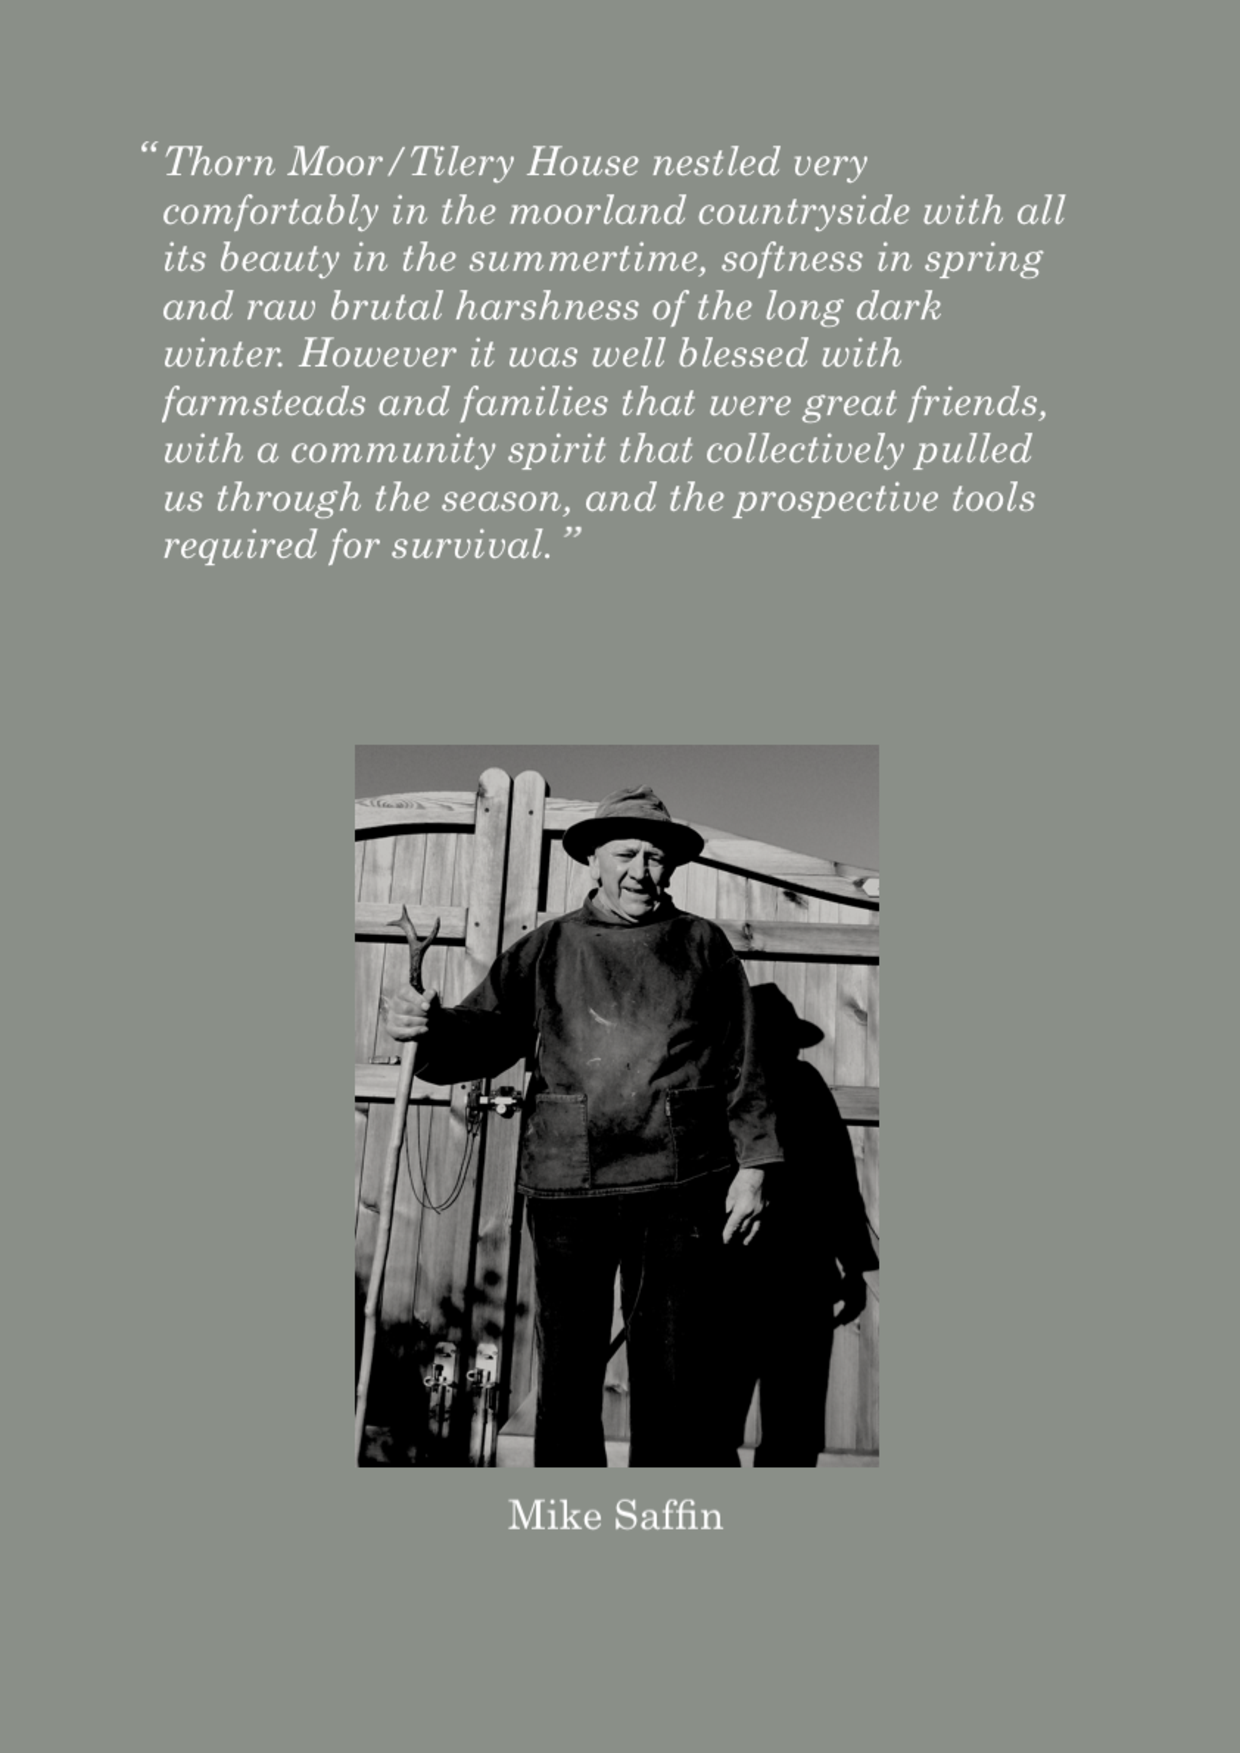
\includepdf{pictures/back-cover.pdf}

\end{document}
